%%%%%%%%%%%%%%%%%%%%%%%%%%%%%%%%%%%%%%%%%%%%%%%%%%%%%%%%%%%%%%%%%%%%%%%%%%%%%%%%
%%%%%%%%%%%%%%%%%%   Vorlage für eine Abschlussarbeit   %%%%%%%%%%%%%%%%%%%%%%%%
%%%%%%%%%%%%%%%%%%%%%%%%%%%%%%%%%%%%%%%%%%%%%%%%%%%%%%%%%%%%%%%%%%%%%%%%%%%%%%%%

% Erstellt von Maximilian Nöthe, <maximilian.noethe@tu-dortmund.de>
% ausgelegt für lualatex und Biblatex mit biber

% Kompilieren mit
% latexmk --lualatex --output-directory=build thesis.tex
% oder einfach mit:
% make

\documentclass[
  tucolor,       % remove for less green,
  BCOR=12mm,     % 12mm binding corrections, adjust to fit your binding
  parskip=half,  % new paragraphs start with half line vertical space
  open=any,      % chapters start on both odd and even pages
  cleardoublepage=plain,  % no header/footer on blank pages
]{tudothesis}


% Warning, if another latex run is needed
\usepackage[aux]{rerunfilecheck}

% just list chapters and sections in the toc, not subsections or smaller
\setcounter{tocdepth}{1}

%------------------------------------------------------------------------------
%------------------------------ Fonts, Unicode, Language ----------------------
%------------------------------------------------------------------------------
\usepackage{fontspec}
\defaultfontfeatures{Ligatures=TeX}  % -- becomes en-dash etc.

% german language
\usepackage{polyglossia}
\setdefaultlanguage{german}

% for english abstract and english titles in the toc
\setotherlanguages{english}

% intelligent quotation marks, language and nesting sensitive
\usepackage[autostyle]{csquotes}

% microtypographical features, makes the text look nicer on the small scale
\usepackage{microtype}

%------------------------------------------------------------------------------
%------------------------ Math Packages and settings --------------------------
%------------------------------------------------------------------------------

\usepackage{amsmath}
\usepackage{amssymb}
\usepackage{mathtools}

% Enable Unicode-Math and follow the ISO-Standards for typesetting math
\usepackage[
  math-style=ISO,
  bold-style=ISO,
  sans-style=italic,
  nabla=upright,
  partial=upright,
]{unicode-math}
\setmathfont{Latin Modern Math}

% nice, small fracs for the text with \sfrac{}{}
\usepackage{xfrac}


%------------------------------------------------------------------------------
%---------------------------- Numbers and Units -------------------------------
%------------------------------------------------------------------------------

\usepackage[
  locale=DE,
  separate-uncertainty=true,
  per-mode=symbol-or-fraction,
]{siunitx}
\sisetup{math-micro=\text{µ},text-micro=µ}

%------------------------------------------------------------------------------
%-------------------------------- tables  -------------------------------------
%------------------------------------------------------------------------------

\usepackage{booktabs}       % \toprule, \midrule, \bottomrule, etc

%------------------------------------------------------------------------------
%-------------------------------- graphics -------------------------------------
%------------------------------------------------------------------------------

\usepackage{graphicx}
\usepackage{grffile}

% allow figures to be placed in the running text by default:
\usepackage{scrhack}
\usepackage{float}
\floatplacement{figure}{htbp}
\floatplacement{table}{htbp}

% keep figures and tables in the section
\usepackage[section, below]{placeins}


%------------------------------------------------------------------------------
%---------------------- customize list environments ---------------------------
%------------------------------------------------------------------------------

\usepackage{enumitem}

%------------------------------------------------------------------------------
%------------------------------ Bibliographie ---------------------------------
%------------------------------------------------------------------------------

\usepackage[
  backend=biber,   % use modern biber backend
  autolang=hyphen, % load hyphenation rules for if language of bibentry is not
                   % german, has to be loaded with \setotherlanguages
                   % in the references.bib use langid={en} for english sources
]{biblatex}
\addbibresource{references.bib}  % the bib file to use
\DefineBibliographyStrings{german}{andothers = {{et\,al\adddot}}}  % replace u.a. with et al.


% Last packages, do not change order or insert new packages after these ones
\usepackage[pdfusetitle, unicode, linkbordercolor=tugreen]{hyperref}
\usepackage{bookmark}
\usepackage[shortcuts]{extdash}

%------------------------------------------------------------------------------
%-------------------------    Angaben zur Arbeit   ----------------------------
%------------------------------------------------------------------------------

\author{Lukas Nickel}
\title{Masterarbeit CTA Kram und so}
\date{2019}
\birthplace{Bielefeld}
\chair{Lehrstuhl für Experimentelle Physik V}
\division{Fakultät Physik}
\thesisclass{Master of Science}
\submissiondate{31. Dezember 2019}
\firstcorrector{Prof.~Dr.~Wolfgang Rhode}
\secondcorrector{Prof.~Dr.~Zweitgutachter}

% tu logo on top of the titlepage
\titlehead{
\includegraphics[height=1.5cm]{logos/tu-logo.pdf}}

\begin{document}
\frontmatter
\maketitle

% Gutachterseite
\makecorrectorpage

% hier beginnt der Vorspann, nummeriert in römischen Zahlen
\thispagestyle{plain}

\section*{Kurzfassung}
\begin{german}
In den letzten Jahrzehnten hat die $\gamma$-Astronomie 
viele Erkenntnisse über die Zusammensetzung des Universums gebracht.
Mitverantwortlich dafür waren die großen Image Air Cherenkov Telescope (IACT)
Experimente der dritten Generation.
In Zukunft soll diese Forschung begleitet und erweitert werden 
durch ein Experiment der nächsten Generation.
Das Cherenkov-Teleskope-Array (CTA) wird die Sensitiviät weiter steigern und den
beobachtbaren Energiebereich erweitern.
In dieser Arbeit werden Rekonstruktionsalgorithmen für CTA vorgestellt und Studien auf 
Monte-Carlo-Daten durchgeführt mit dem Fokus auf der frühen Phase des Experimentes.
Zu Beginn werden nur wenige Teleskope errichtet sein, sodass Ereignisse nur 
mit wenigen Teleskopen gesehen werden.
\end{german}

\section*{Abstract}
\begin{english}
In the past years the $\gamma$-astronomy has lead to many interesting
insights about the fundamental processes of the universe.
Part of that were the big imaging air cherenkov telescopes (IACTs) 
of the third generation.
In the future this research will be expanded with a next generation experiment.
The Cherenkov Telescope Array (CTA) will improve the sensitivity and
expand the observable energy range.
In this work we will present reconstruction algorithms for CTA und perform 
studies on monte carlo data with the focus on the early stages of the experiment.
In this stages CTA will only have some of the planned telescopes installed
leading to low multiplicity events.
\end{english}

\tableofcontents

\mainmatter
% Hier beginnt der Inhalt mit Seite 1 in arabischen Ziffern
\chapter{Gamma Astronomy}

\section{The Field of Astroparticle Physics}

The ballon flights of Victor Hess \cite{Hess:1912srp} are
often times cited as the starting point of astroparticle physics,
because they gave reason to believe, that the measured ionizing
radiation is of extraterrestrial origin. 

The radiation was referenced as "Höhenstrahlung" 
(see e.g. \cite{myssowsky1926versuche}) 
and "cosmic rays" (see e.g. \cite{millikan1928origin}) with 
the english term cosmic rays eventually winning out.

Soon after, in 1933, Carl D. Anderson discovered the existence
of antimatter using a cloud chamber \cite{PhysRev.43.491},
which is crucial for the measurement of especially
high energy photons.

Later years brought the discovery of several new particles,
that are imperative to modern astronomy:
pions \cite{LATTES1947}, muons \cite{PhysRev.52.1003}
and neutrinos \cite{Cowan103}.

Recently, the so far last discovery on this journey
was made with the measurement of the first gravitational 
waves \cite{PhysRevLett.118.221101}.

This leaves the field of astronomy with four different
messengers, which coins the term
multi messenger astronomy:
\begin{enumerate}
	\item Electromagnetic radiation
	\item Cosmic rays
	\item Neutrinos
	\item Gravitational waves
\end{enumerate}

Figure \ref{fig:multi_messenger} illustrates the key differences between
photons, protons and neutrinos.
This thesis focuses on the detection of cosmic and gamma rays.

\begin{figure}
	\centering
	\captionsetup{width=0.9\linewidth}
	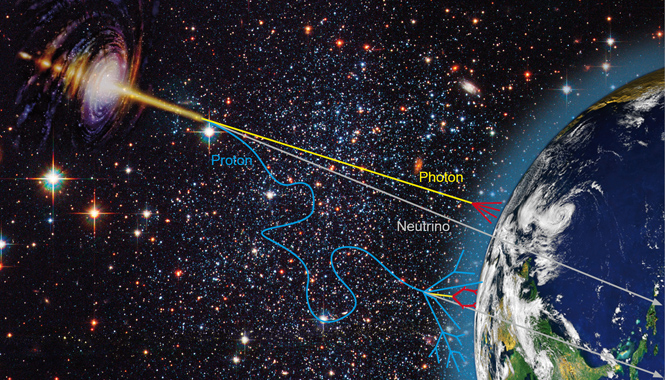
\includegraphics[width=0.9\textwidth]{images/astro-web-titel.jpg}
	\caption{Visualization of the behaviors of different messengers
		particles in modern astronomy.
		Photons and neutrinos travel through the universe without deflection,
		because they do not carry an electric charge.
		Neutrinos interact less than photons,
		which leads to a high proportion passing through earth.
		Charged cosmic rays get deflected by interstellar
		magnetic fields and thus generally do not allow for a reconstruction
		of the source position.
		The image is taken from the DESY-website at \cite{desy_mm_astro}.
	}
	\label{fig:multi_messenger}
\end{figure}

In contrast to charged cosmic rays, $\gamma$-rays point towards
their sources, allowing to search for bright sources of radiation.
This makes it possible to learn more about the acceleration processes
and sources, that produce high energy gamma and cosmic rays.
Two important classes of proposed sources are active galactic nuclei,
which are considered massive black holes, that produce jets and 
supernove remnants. (mehr research)

Researching the diffuse component of gamma-rays on the other hand holds
potential to find out more about interstellar magnetic fields and the
propagation of relativistic particles in the universe.

Another motivation to research gamma-rays lies in the assumption, that
dark matter could annihilate to photon pairs. (quelle im tu netz öffnen)

Due to the way gamma-rays are being detected, it is not possible
to avoid measuring cosmic rays as well.
At the same time cosmic rays are much more numerous,
which makes them the dominant background in gamma astronomy \cite{funcray}.

\section{Production of Gamma-Rays}
Creation of high-energy gamma-rays can not happen thermally,
but happens in a combination of high energy charged particles 
and interstellar targets or magnetic fields \cite{funcray}.
A model for the production at the source, the Self Synchroton Comptoon model,
focuses on photon emission from an initial pure electron distribution.
The key aspects of this model are now briefly presented. 

\textbf{Synchroton Radiation}

Propposed sources of cosmic and gamma rays include 
high magnetic fields. Any moving charged particle will thus be
deflected perpendicular to its moving direction
due to the Lorentz-force, forcing them on a radial trajectory.
At the same time a relativistic charged particle, 
that gets accelerated radially, emits synchroton 
photons with average energy given by:

\begin{equation}
	\langle E_{\gamma} \rangle \propto \frac{1}{M_P} E_P^2 B^2.
	\label{eq:synchroton}
\end{equation}

Here, $M_P$ and $E_P$ denote the accelerated particle's 
mass and energy respectively. With the inverse mass dependency 
it is immediately evident that
synchroton radiation plays a major role in leptonic 
emission and much less in hadronic emission.

A direct result of this is, that the electrons energy gets reduced
in the process, affecting ("cooling") the initial electron distribution.
This is sometimes referred to as synchroton cooling.

The emitted synchroton spectrum needs to be further modified 
if the emitting region is optically thick and photons 
get absorbed by the medium.
This is in fact always the case, as the regions contains 
both magnetic fields and a high density of electrons.

\textbf{Inverse Compton Scattering}
In a classical particle interpretation photons and electrons 
can collide exchanging energy and altering their directions.
For the normal case of Compton scattering the electron 
is assumed to be at rest and the photon can never gain 
energy by colliding with the electron.
This can be 
seen by the increase in wavelength in \eqref{eq:compton},
with $\lambda^{\prime}$ denoting the scattered photons 
wavelength, $\lambda$ denoting the initial photons wavelength  
and $\Theta$ denoting the scattering angle.

\begin{equation}
	\lambda^{\prime} - \lambda  \propto \left(1-\cos{\Theta} \right)
	\label{eq:compton}
\end{equation}

If the electron itself is moving with much higher energy
than the photon, this changes and the photon can gain substantial energy.
This is reffered to as inverse Compton scattering.
In that case, transforming the equations to the 
electron's frame of reference and back to the laboratory frame of reference
boosts the photons energy by a factor $\gamma$ for each transformation, 
with $\gamma$ being the Lorentz factor of the electron.

A limit to the photon energies is set by the scattering cross
section, which reduces with higher photon energies.
For low energies the cross section can be approximated by 
the Thomson cross section, for high energies
one uses the Klein-Nishina cross section. (quellen angeben)

The Synchroton Self Compton model combines the above mentioned
effects to produce a photon energy distribution from an
electron distribution, which is often times assumed to
follow a power-law spectrum initially.
The free parameters of the model can be interpreted as 
three frequencies: The minimum injection frequency $\nu_m$, 
the cooling frequency $\nu_c$ and the self-absorption frequency $\nu_a$.
Depending on the order of these parameters, different 
photon distributions can be generated.

A detailed analysis of the influence of the parameters of
the Synchroton Self Compton model, can be found in 
\cite{10.1093/mnras/stt1461}.


\section{Experiments for Cosmic and Gamma Rays}
Emitted $\gamma$-rays can be observed either directly
from outside the atmosphere via satellites or indirectly
via ground based gamma astronomy.

The different types of experiments differ in the way particles are detected and
the resulting energy ranges, where they are most sensitive.

\subsection{Satellite Experiments}
Satellite experiments allow direct measurements of gamma and cosmic rays, because of the operation
above the atmosphere.
This allows to use similar techniques as experiments located at terrestrial 
particle detectors: Incoming photons hit an initial layer and produce an electron pair 
via pair production. The tracks of these particles get observed before they reach the calorimeter,
where their energies get measured.

Despite the advantages over ground based experiments, the small detector areas 
limit the sensitivities at higher energies.

A currently operating example is the FERMI Gamma-ray Space Observatory (FGST) \cite{Atwood_2009}.
The Large Area Telescope (LAT) on 
the FGST covers an energy range of
\SI{20}{\mega\electronvolt} to \SI{100}{\giga\electronvolt} \cite{Atwood_2009}.
It is able to cover a huge field ov view (fov) of 
\SI{20}{\degree}. A second detector, the Gamma-ray Burst Monitor,
searches for gamma ray bursts using a scintilator setup to notify other experiments.

\subsection{Imaging Air Cherenkov Telescopes (IACTs)}
A class of ground-based observatories are the 
Imaging Air Cherenkov Telescopes (IACTs),
which will be the focus of this thesis.

In constrast to the satellite experiments, they cannot directly
observe the cosmic particle. Instead they use the atmosphere as detector medium.
High energy primary particles generate a cascade of secondary particles
when interacting with the atmosphere. These particles generate cherenkov
light, which is recorded by the IACTs.

Modern experiments include 
MAGIC \cite{ALEKSIC2012435},
VERITAS \cite{WEEKES2002221}
and HESS \cite{vincent2005hess},
all of which consist of multiple telescopes to observe the shower 
from different angles to improve the reconstruction.

The observable energy range generally generally lies in the range of
some \SI{10}{\giga\electronvolt} to some 10-\SI{100}{\tera\electronvolt}.

\subsection{Air Shower Arrays}
Air shower arrays, like IACTs, operate on the ground and thus also have 
to measure the particle indirectly.

In contrast to IACT-experiments, air shower arrays consist of a huge
number of single scintillation detectors, spaced on a grid on the ground.
Instead of the cherenkov light, they measure the
remaining particles of the shower. This makes them feasible
for energies even above the ones measured by IACTs.

A modern experiment is the High Altitude Water Cherenkov Observatory (HAWC) \cite{2015ICRC...34..966S}.
It uses \num{300} water tanks to measure air showers with a lower threshold
of under \SI{1}{\tera\electronvolt}.

\section{Detection of Gamma Rays with IACTs}
% \subsection{Detecting Gamma Rays}
\label{sec:measuring}

The primary particles of gamma or cosmic rays cannot be 
observed with IACTs directly. Instead one can measure the secondary particles
that emerge from the particles interaction with matter.

If the primary particle energy is high enough, the resulting 
secondary particles can interact with the atmosphere themself, thus starting a 
cascade of secondary particles.
Particles, that have enough energy, are faster than the local speed of light.
Because the electrons carry a charge and the air acts as dielectricum, 
cherenkov light gets emitted \cite{quelle suchen}.

Cherenkov photons get collected by the mirror(s) of a telescope
and projected onto a camera system mounted above the mirror.
Figure \ref{fig:iact_mirror_camera} illustrates the measurement of 
an air shower.

\begin{figure}
	\centering
	\captionsetup{width=0.9\linewidth}
	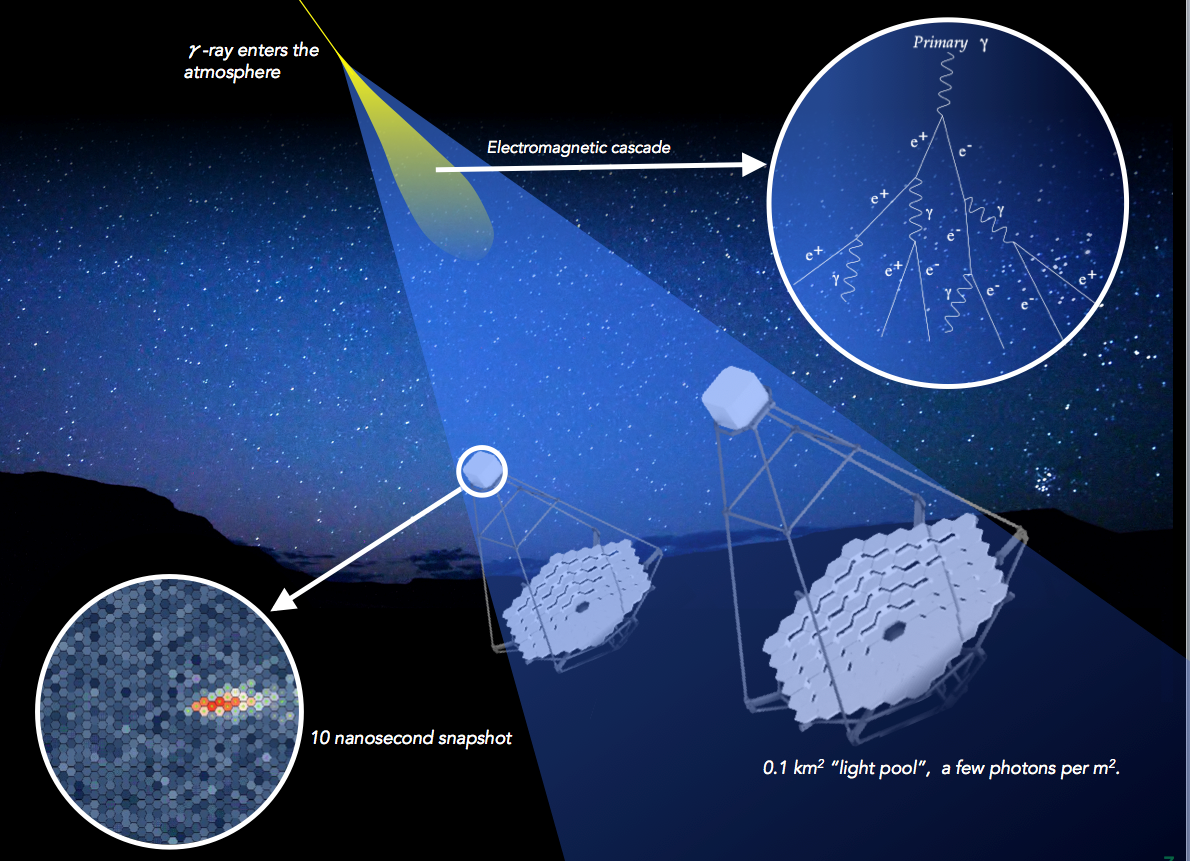
\includegraphics[width=0.9\textwidth]{images/cta47.png}
	\caption{A schematic illustration of the working principles of 
	an IACT experiment:
	A $\gamma$-ray produces an air shower in the atmosphere
	that points roughly towards the telescopes.
	Cherenkov light from the air shower 
	hits the mirrors and gets focused into a camera mounted on top.
	An illustration of the resulting image after integrating 
	\SI{10}{\nano\second} of the pixel measurements
	can be seen in the left bottom corner.
	The image is taken from the CTA-website \cite{cta_web}.}
	\label{fig:iact_mirror_camera}
\end{figure}

Depending on whether the primary particle is 
a photon/electron or a heavier, hadronic particle such as a proton 
or iron core, the interactions in the atmosphere and the 
produced secondary particles vary.

This leads to a separation of electromagnetic and hadronic showers.
If the experiment is primarly looking for 
gamma rays, e.g. if measuring a known source like the Crab Nebula, 
the hadronic showers act as dominant background.
As hadronic showers get observed much more frequently, 
the identification of the primary particle type is a very important 
task, often times referred to as gamma-/hadron-separation.

\subsection{Electromagnetic Showers in the Atmosphere}
Electromagnetic showers consist mainly of two types of particles:
\begin{enumerate}
	\item{Photons $\gamma$}
	\item{Electrons $e^-$ / Positrons $e^+$}
\end{enumerate}

The main interaction for high energy photons is pair 
production, generating an $e^+/e^--$pair where the summed energy of 
the lepton pair equals the photon energy.
On the other hand high energy electrons lose 
most of their energy by radiating bremsstrahlung, leading to a photon with 
an energy close to the electron energy.
Only at lower particle energies other interaction forms show their impact,
with particle scattering and ionization 
leading to more continuous energy losses.

These assumptions lead to the most basic model of an 
electromagnetic shower, proposed by Bhabha and Heitler in 1937
\cite{doi:10.1098/rspa.1937.0082}.
It starts with a high energy primary photon before its interaction in the atmosphere 
and continues the calculation in discrete epochs.
The photon produces a pair of $e^-$ and $e^+$ in the first epoch.
Because of the high energies at play, the direction of these secondary 
particles does not deviate significantly from the photon's direction, 
making the problem essentially one-dimensional.
The $e^+/e^-$ continue on to radiate a photon each and the cycle continues.
Each step doubles the number of particles in the shower with each particle 
on average getting half the energy of its parent particle.
These processes continue until the energy of the $e^+/e^-$ becomes low enough for
continuous ionization processes to become relevant.
At this point the particle is considered to be stopped and the shower
does not evolve further.

Today monte carlo calculations get used to simulate the properties 
of particle showers in the atmosphere.
The most common software to model the atmospheric interactions is
CORSIKA \cite{Engel:2018akg}.

Figure \ref{fig:gamma_shower} illustrates the Bhabha-Heitler model (left)
and a \SI{100}{\giga\electronvolt} gamma shower, simulated with CORSIKA (right).

\begin{figure}
	\centering
	\captionsetup{width=0.9\linewidth}
	\begin{subfigure}{.7\textwidth}
  		\centering
  		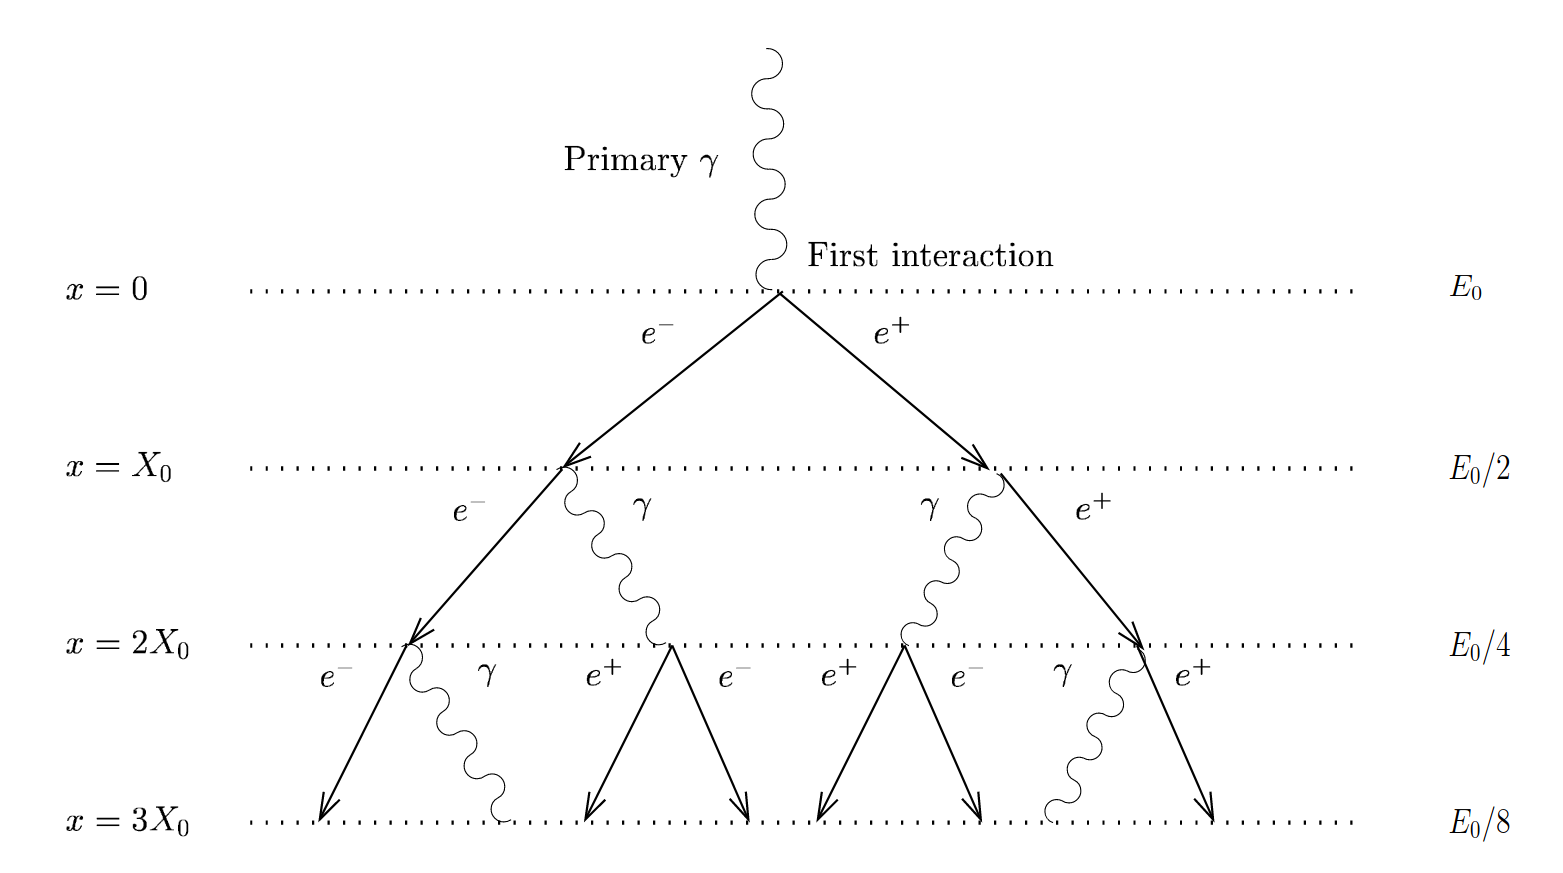
\includegraphics[width=\linewidth]{images/em_shower_illustration.png}
	\end{subfigure}%
	\begin{subfigure}{.2\textwidth}
 		\centering
		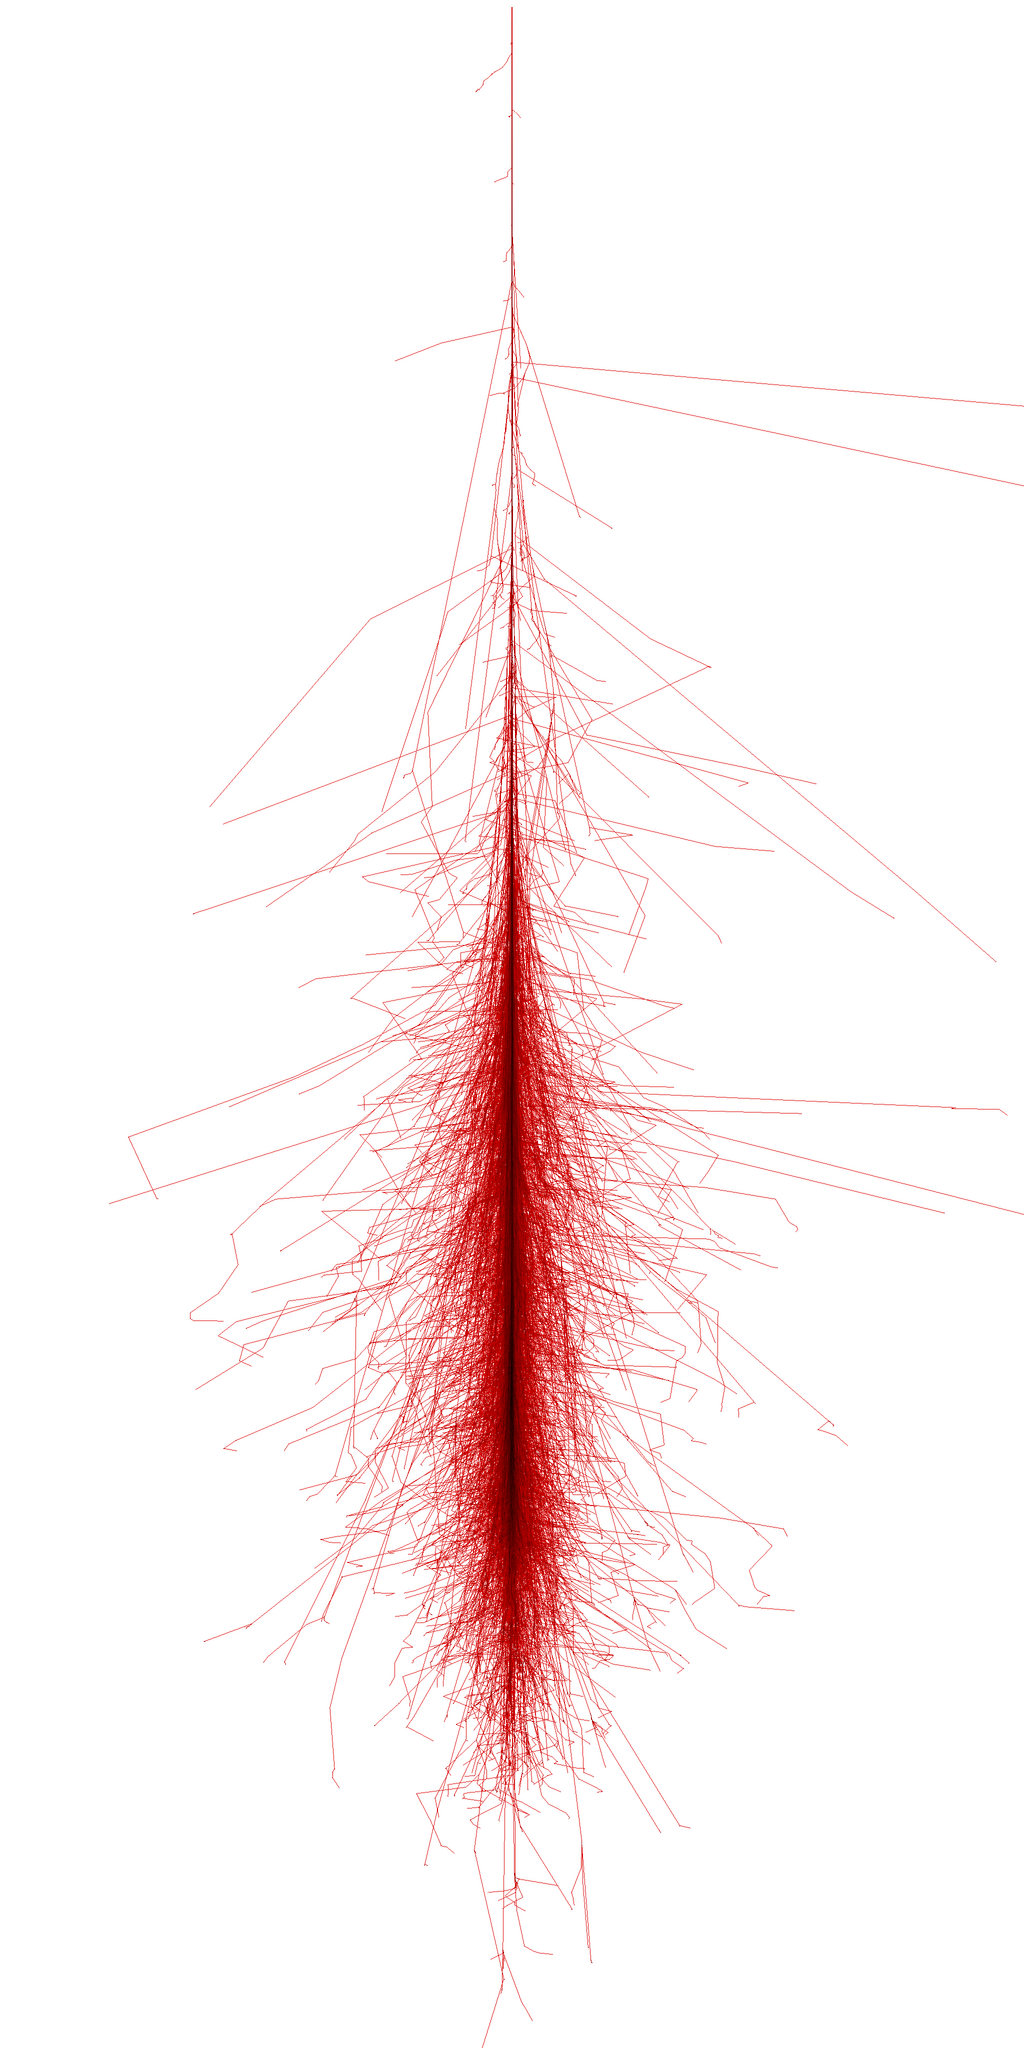
\includegraphics[width=\linewidth]{images/corsika_100gev_photon.png}
	\end{subfigure}
	\caption{
		Left: A schematic illustration of the first epochs of the 
		Bethe-Heitler shower model with equal radiation lengths for
		bremsstrahlung and pair production.
		The image is taken from an inaugural thesis 
		by Stefan Funk \cite{funk_doctor}. \\
		Right: A \SI{100}{\giga\electronvolt} gamma-shower as xz-projection, simulated with CORSIKA.
		The shower is relatively contained with only little extent perpendicular 
		to the shower direction (z-axis). The image is taken from 
		the CORSIKA-website \cite{corsika_showers}}
	\label{fig:gamma_shower}
\end{figure}

\subsection{Hadronic Showers in the Atmosphere}
Hadronic showers include all the interactions known from 
electromagnetic showers, but add nuclear interactions on top.
These lead to non-negligible additional energy losses 
and the creation of secondary hadronic particles.

Approximations are more difficult to do and monte carlo simulations 
become the only way to reasonably calculate shower behavior.

At the end of the shower a relevant portion of the particles have decayed into the 
lightest hadronic particles, pions ($\pi^0, \pi^+, \pi^-$), of which the neutral pions 
rapidly decay into photons.
This means that a part of the hadronic shower
eventually becomes an electromagnetic subshower.

Figures \ref{fig:proton_shower}
shows some of the particles generated in a hadronic shower (left)
and a \SI{100}{\giga\electronvolt} proton shower, simulated with CORSIKA (right).

\begin{figure}
	\centering
	\captionsetup{width=0.9\linewidth}
	\begin{subfigure}{.7\textwidth}
  		\centering
  		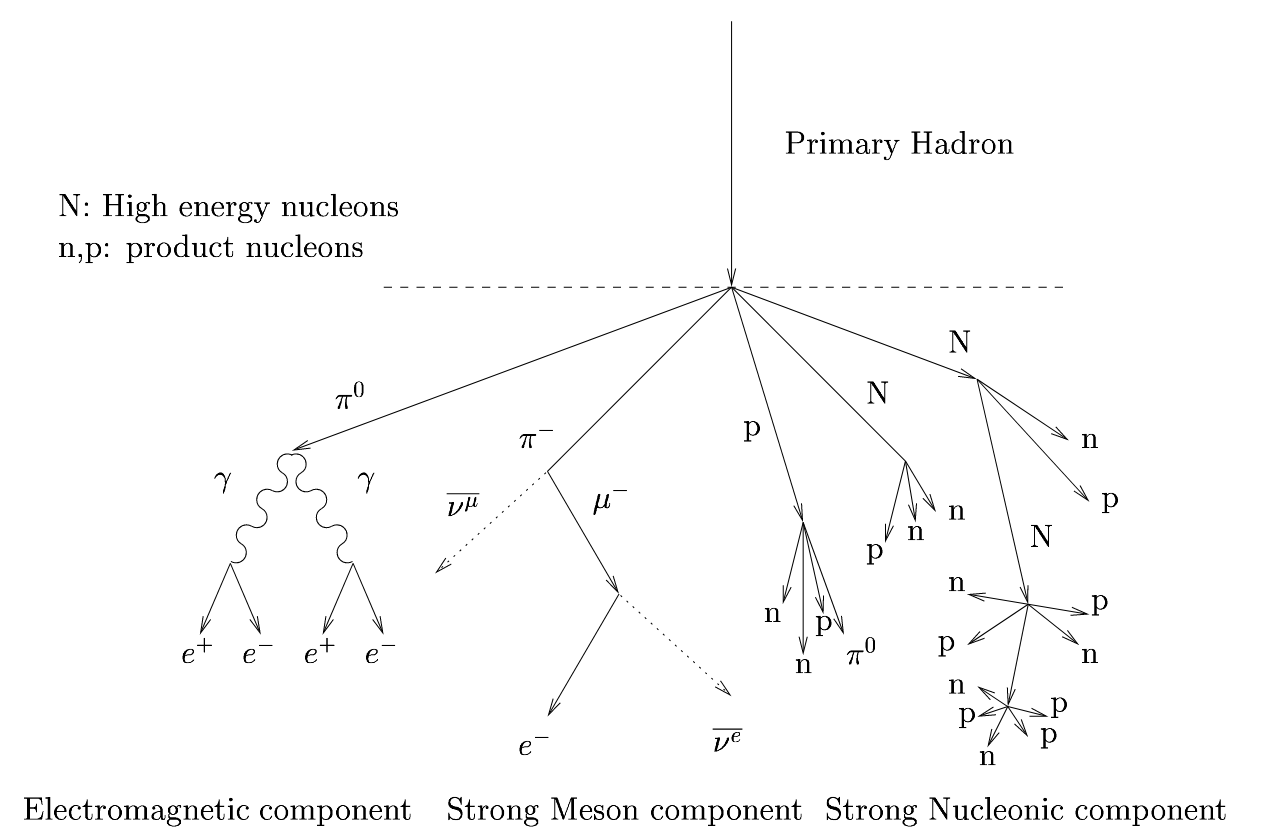
\includegraphics[width=\linewidth]{images/hadron_shower_illustration.png}
	\end{subfigure}%
	\begin{subfigure}{.2\textwidth}
 		\centering
		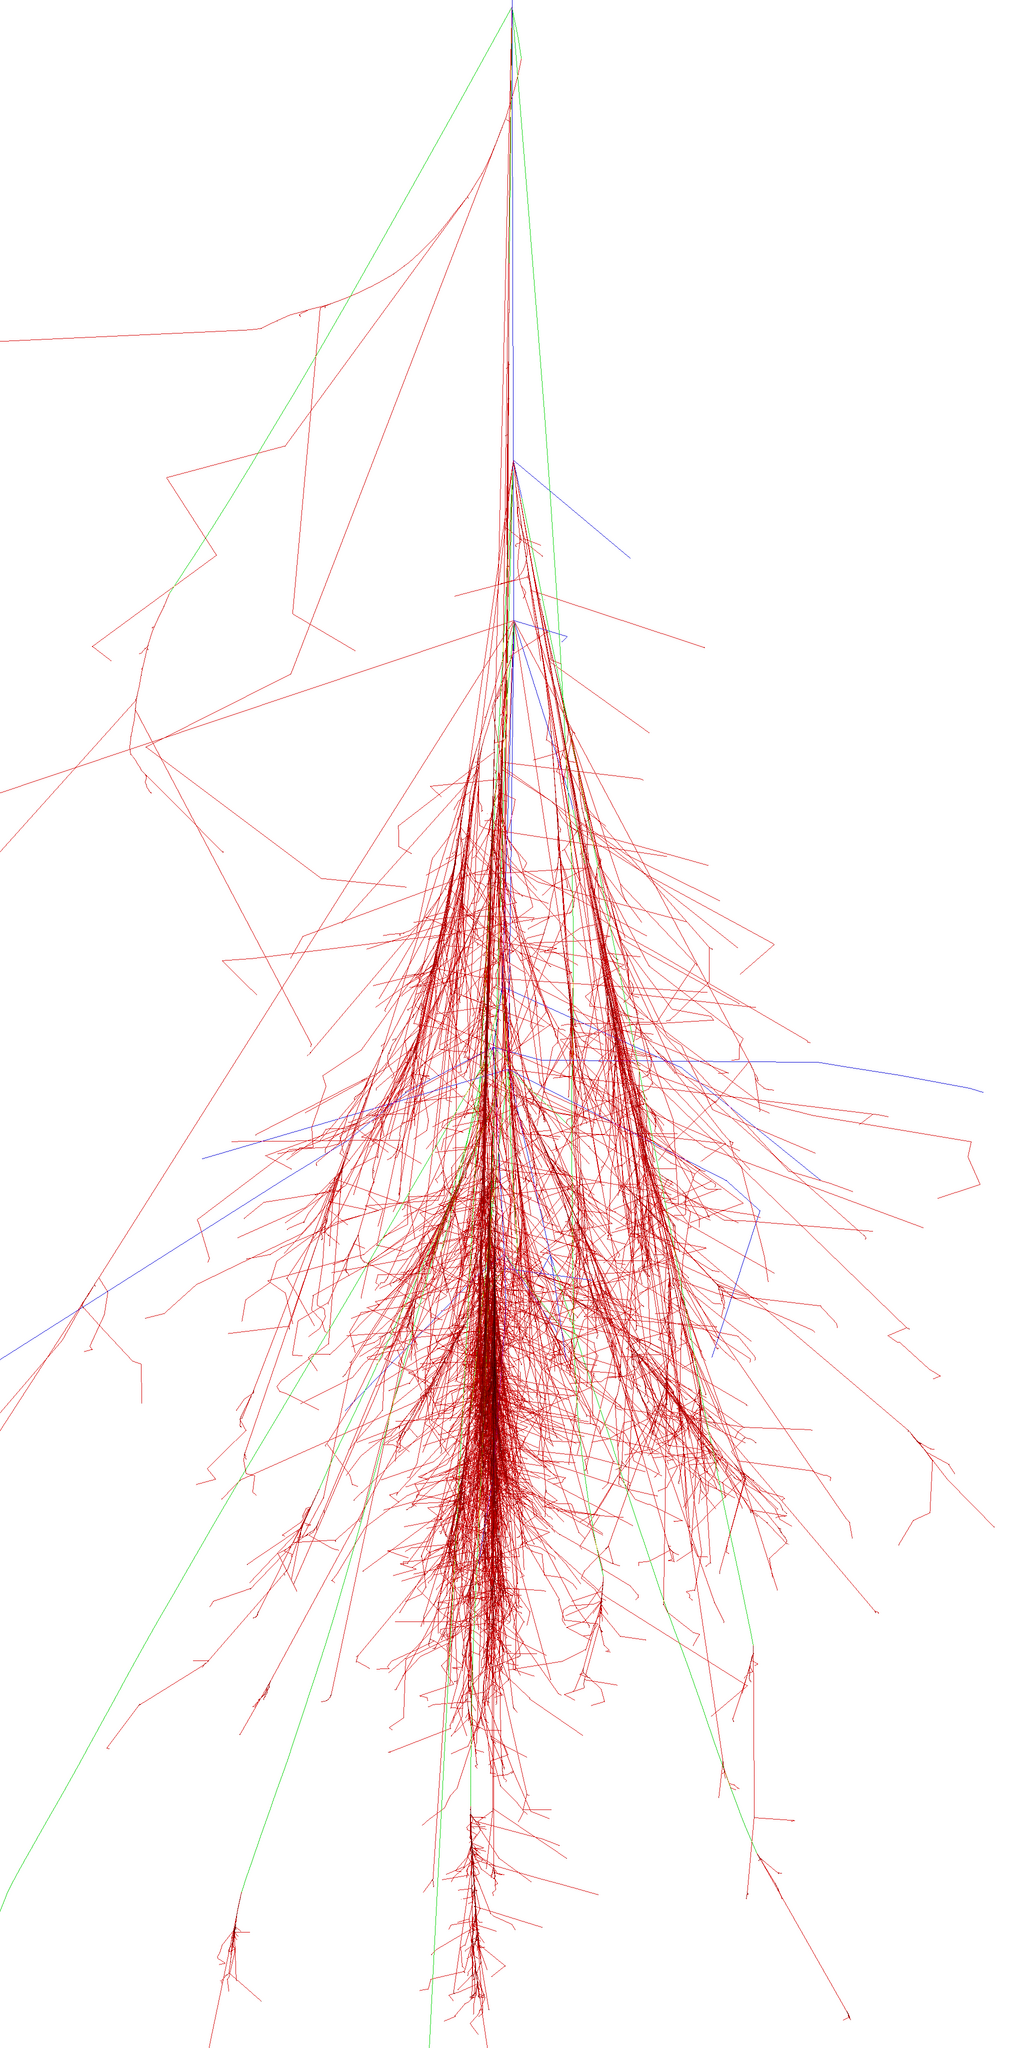
\includegraphics[width=\linewidth]{images/corsika_100gev_proton.png}
	\end{subfigure}
	\caption{
		Left: A purely qualitative,
		schematic illustration of the generation of a hadronic shower.
		It shows how the primary hadron generates different subshowers
		with vastly different particles.
		The image is taken from an inaugural thesis 
		by Stefan Funk \cite{funk_doctor}.\\
		Right: A \SI{100}{\giga\electronvolt} proton-shower as xz-projection,
		simulated with CORSIKA.
		The shower is less contained than the gamma shower of equal energy in 
		figure \ref{fig:gamma_shower}.
		Different colors indicate different particle types.
		The image is taken from 
		the CORSIKA-website \cite{corsika_showers}.}
	\label{fig:proton_shower}
\end{figure}





\chapter{IACT Experiments}
\label{cta}

sensitivity in crab flux angeben

\section{The Current Generation}

Towards the end of the 1990s several third generation experiments were
proposed:
H.E.S.S and MAGIC, deriving from parts of the HEGRA collaboration, 
VERITAS from Whipple and the no longer operating CANGAROO from Adelaide and 
several japanese universities \cite{HILLAS201319}. All of these
were designed as stereoscopic imaging telescopes building on the progress made during the 
earlier experiments with two experiments located on each the north and the south hemisphere.

\subsection{Major Atmospheric Gamma Imaging Telescopes (MAGIC)}
MAGIC is a experiment nowadays operating as a stereo setup of two telescopes.
The two telescopes are located at La Palma and have a \SI{17}{\meter} diameter mirror setup each \cite{ALEKSIC201676}.

In the first phase MAGIC consisted of a single telescope, for differentiation usually
referred to as MAGIC-I. This first phase started 
operation in 2004 and had MAGIC-I be the largest IACT of its time.

The addition of MAGIC-2, the second mostly identical telescope, in 2009 marked the 
start of the second phase of the experiment and the transition to a third 
generation experiment \cite{2009arXiv0907.1211C}.
In the second phase MAGIC operates in the energy range from \SI{30}{\giga\eV}
up to \SI{100}{\TeV} \cite{magic_website}.

The DISP-method for the reconstruction of the event arrival direction 
was significantly improved by including timing information and showed better 
results for stereoscopy than the simple crossing of the main shower axis \cite{ALEKSIC2012435}.

A specialty of the MAGIC experiment lies in its ability to 
perform fast skews and thus react to gamma ray bursts after they have been observed 
by satellite experiments \cite{2003ICRC....5.2943B}.
This enabled the recent observation of the very first \si{\TeV}
gamma ray burst observed with IACTs \cite{collaboration2019teraelectronvolt}.


\subsection{Very Energetic Radiation Imaging Telescope Array System (VERITAS)}
VERITAS	was initially planned as a seven-telescope array, arranged in a diamond shape
\cite{WEEKES2002221}.

Eventually the collaboration settled 
with four telescopes. 
Each telescope covers a 3.5° FoV with a \SI{12}{\meter} diameter mirror and 
a 499 pixel PMT camera.

A relocation of telescope 1 in 2009 meant that the 
experiment made better use of the given area and its four telescopes,
improving the sensitivity by up to 30\% \cite{2009arXiv0912.3841P}.
The old and new layout can be seen in figure \ref{fig:veritas_relocation}.

The VERITAS collaboration mentions a lower threshold of \SI{100}{\giga\electronvolt}
with the four telescope setup.

\begin{figure}
	\center
	\captionsetup{width=0.9\linewidth}
	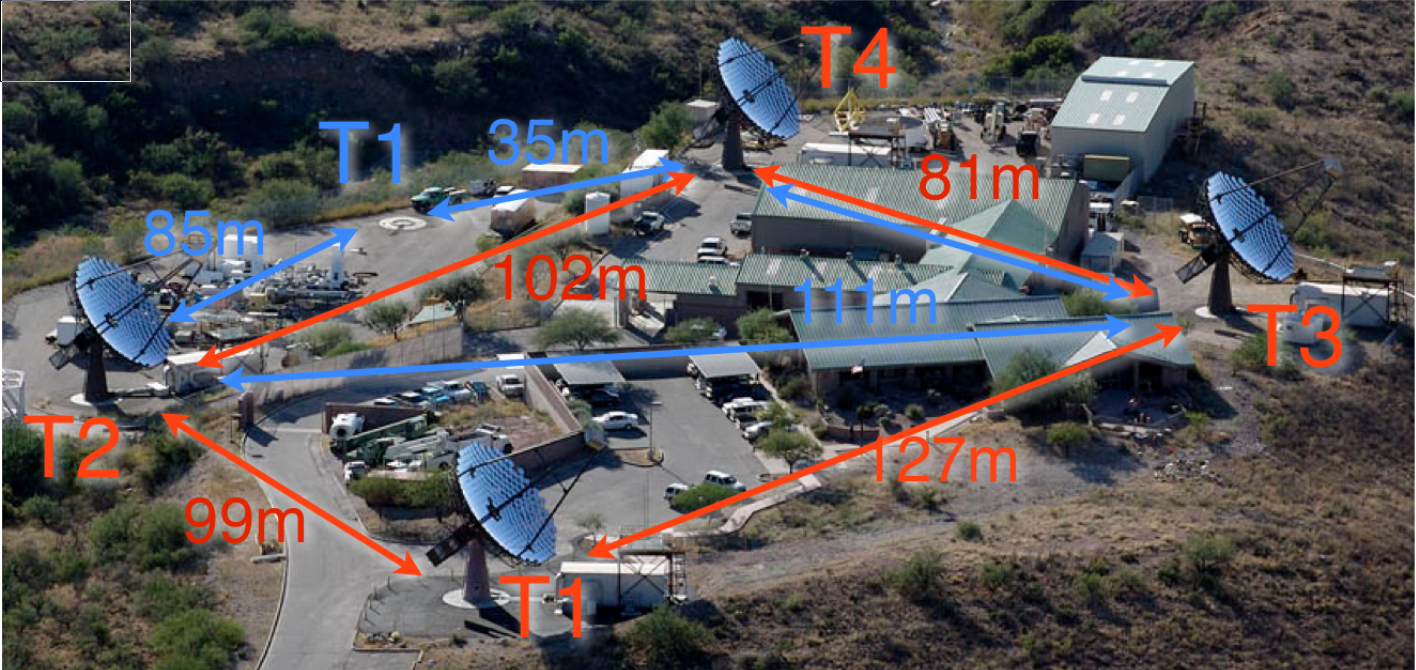
\includegraphics[width=.9\textwidth]{images/veritas_relocation.png}
	\caption{The VERITAS array layout after relocation of the first 
		telescope. The distances between the telescopes are 
		highlighted for the old(blue) and the new(red) array.
		In the old setup the telescopes T1, T2 and T4 were too closely
		located, making their measurements redundant.
	 	The image is taken from an official paper, that investigates
		the improved performance gained by relocating the telescope \cite{2009arXiv0912.3841P}.}
	\label{fig:veritas_relocation}
\end{figure}

Like MAGIC, VERITAS makes use of the DISP-method, especially at large zenith angles 
\cite{2015ICRC...34..771P}.

\subsection{High Energy Stereoscopic System (HESS)}

The HESS experiment consists of five telescopes and 
is - in contrast to MAGIC and VERITAS - operating in the southern 
Hemisphere, in Namibia.

A similar distinction in phase I and phase II as with MAGIC can be taken with 
HESS phase I consisting of four \SI{13}{\meter} diameter telescopes,
arranged at the edge of a square of \SI{120}{\meter} long sides \cite{HINTON2004331}.
These operated from 2004 to 2012 when the experiment went into phase II.

Phase II brought the larger, fifth telescope with the aim to lower the energy threshold
further. This $\SI{24}{\meter} \times \SI{32}{\meter}$-mirror telescope 
was placed in the middle of the other telescopes.
HESS operates at a similar energy range as MAGIC, stating a lower threshold as low as 
\SI{20}{\giga\electronvolt} \cite{vincent2005hess}.


\section{Next to come: The Cherenkov Telescope Array (CTA)}
\label{sec:cta}

The Cherenkov Telescope Array aims to be a next generation IACT experiment.
With two sites of operation, one for each hemisphere, and a number of different 
telescopes proposed, CTA is going to expand on the findings of the third 
generation experiments.

Like HESS in phase II, the CTA arrays are going to consist of different sized telescopes, namely
the Large Sized Telescope (LST, \SI{23}{\meter}), 
the Medium Sized Telescope (MST, \SI{12}{\meter}) 
and the Small Sized Telescope (SST, \SI{4.3}{\meter}).

Extensive Monte Carlo simulations have been performed to find optimal array arrangements
\cite{BERNLOHR2013171}.

The currently planned layouts at LaPalma and in Chile are shown in 
\ref{fig:cta_layout}.
The expected sensitivity compared against other currently operating
experiments is shown in figure \ref{fig:cta_performance}.

\begin{figure}[H]
	\center
	\captionsetup{width=0.9\linewidth}
	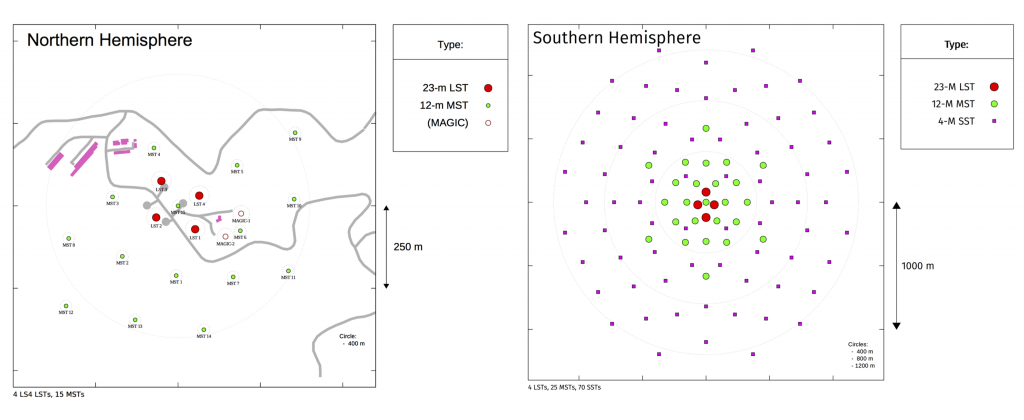
\includegraphics[width=0.9\textwidth]{images/cta_layout.png}
	\caption{
	Left: The array on the northern hemisphere. It will be build at LaPalma
	and feature only LSTs and MSTs.
	Right: The array at the southern hemisphere.
	It will consist of more telescopes and thus 
	work at a bigger energy range.
	The image is taken from the CTA-website \cite{cta_web}.}
	\label{fig:cta_layout}
\end{figure}

\begin{figure}[H]
	\center
	\captionsetup{width=0.9\linewidth}
	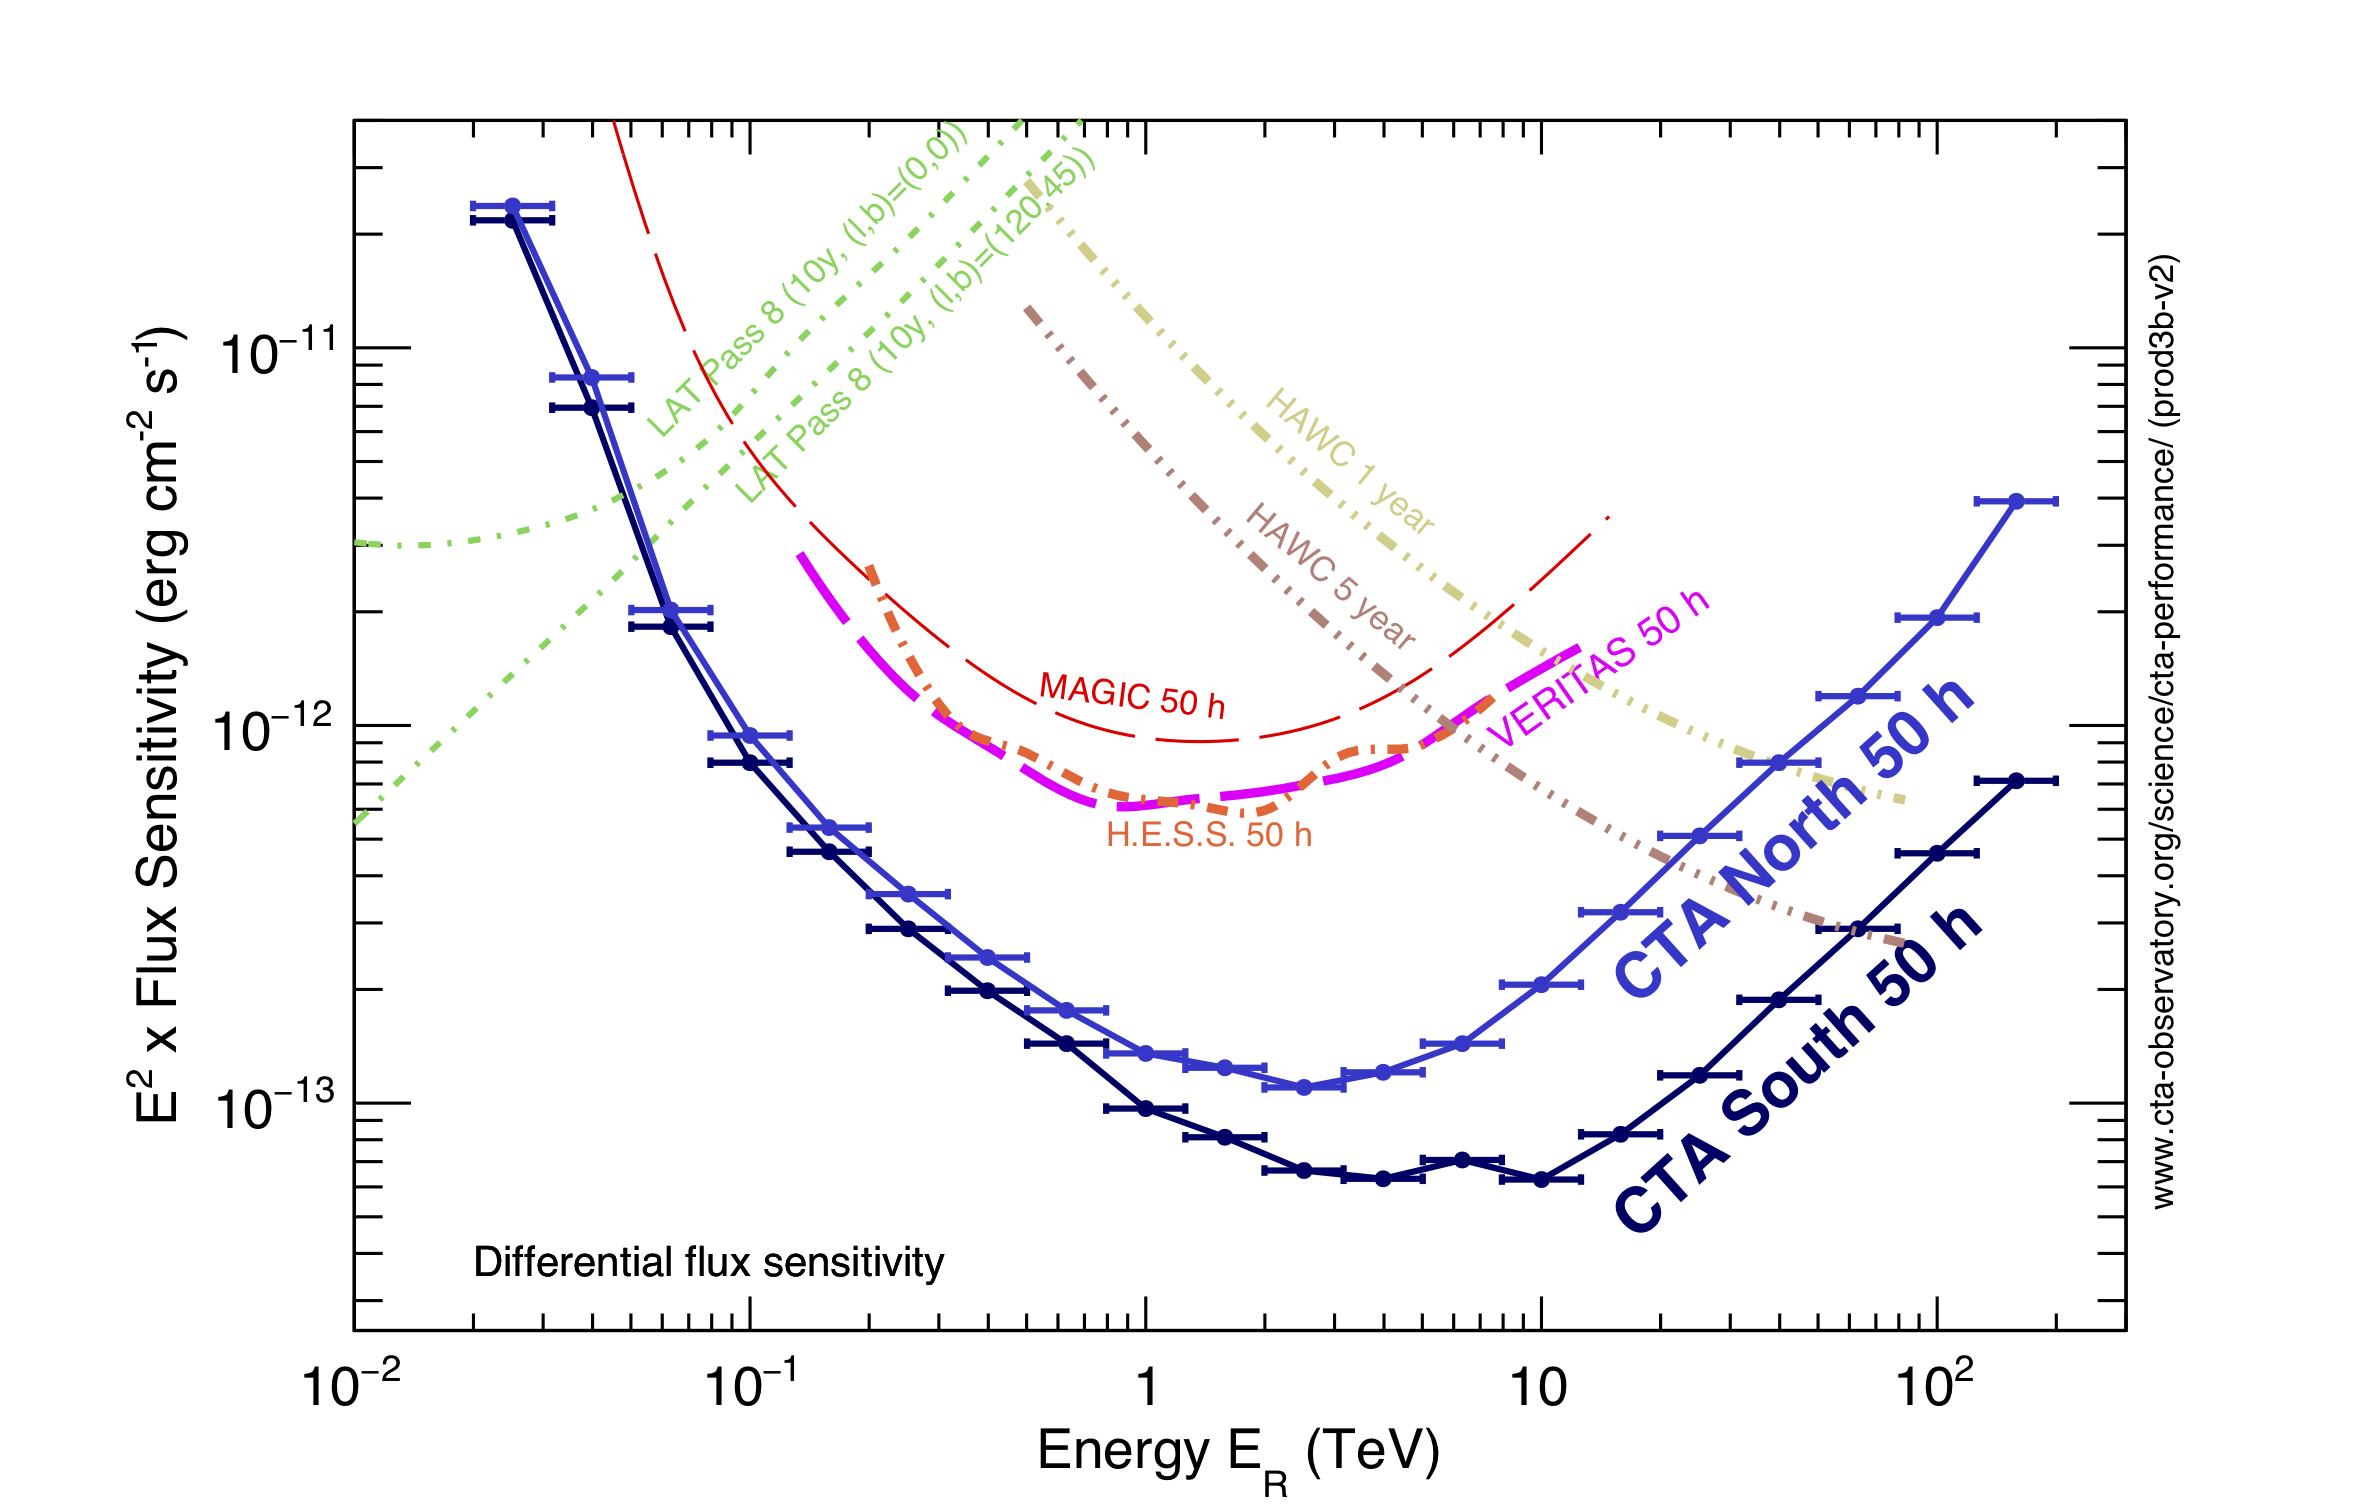
\includegraphics[width=0.9\textwidth]{images/cta_performance.png}
	\caption{A rough comparison of the expected differential sensitivity of CTA compared against
	other experiments. The differential sensitivity is defined as the
	minimum required flux to detect a point source with 5$\sigma$.
	The image is taken from the CTA-website \cite{cta_web}.}
	\label{fig:cta_performance}
\end{figure}

%\newpage
\subsection{LST}
\label{sec:lst}
The Large-Sized Telescope is going to be biggest telescope of CTA
with a mirror diameter of \SI{23}{\meter}.
It will provide the best sensitivity in the energy range from 
\SI{20}{\giga\electronvolt} to \SI{150}{\giga\electronvolt} with a field of view of \SI{4.3}{\degree}.
The camera of the LST, the LSTCamera, has \num{1855} channels 
with \num{265} photomultiplier tubes \cite{cta_web}.

The readout electronic is based on the Domino Ring Sampler 
Version 4 chip, which is also used by the MAGIC experiment
\cite{Kubo:2013pwa}. 

Since the LST is looking for the lowest energy $\gamma$-rays, it needs
very large mirror areas. At the same, time the effective detector area does 
not need to be as high as for higher energy events.
For this reason only 4 telescopes are planned per array.

The first LST has been inaugurated at the 10 October 2018 in La Palma \cite{lst_debut}.
It is foreseen to be the first telescope to be operated by the CTA Observatory.
Until the it has to undergo a critical design review to make sure the performance 
complies with the requirements and expectations.

\begin{figure}
		\centering
		\captionsetup{width=0.9\linewidth}
		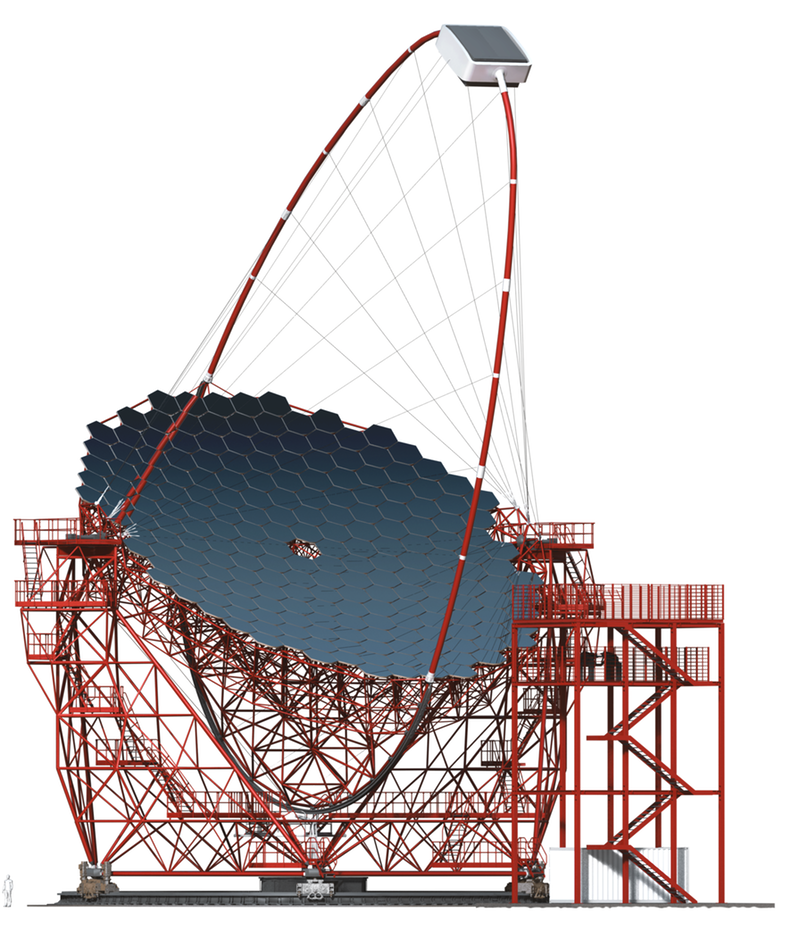
\includegraphics[width=.5\textwidth]{images/LST.png}
		\caption{
			An illustration of the Large Sized Telescope (LST) with its
			\SI{23}{\meter} diameter parabolic mirror.
			In the lower left corner a human is included for scale.
			The image can be found at the official CTA-website \cite{cta_web}.}
		\label{fig:lst}
\end{figure}

%\newpage
\subsection{MST}

\begin{wrapfigure}{R}{0.5\textwidth}
	\centering
	\captionsetup{width=0.9\linewidth}
	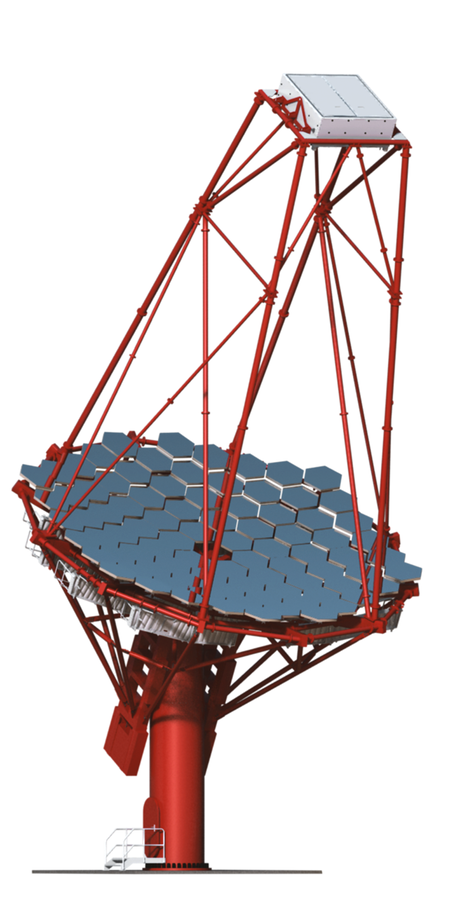
\includegraphics[width=.4\textwidth]{images/MST-1.png}
	\caption{An illustration of the Mediium Sized Telescope (MST) with its
	\SI{11.5}{\meter} diameter mirror.
	The mirror design is based on the Davies-Cotton design.
	The image can be found at the official CTA-website \cite{cta_web}.}
	\label{fig:mst}
\end{wrapfigure}

The Medium-Sized Telescopes (MST) are primarily going to look at the 
energy range from \SI{150}{\giga\electronvolt} to \SI{5}{\tera\electronvolt}.
A total of 15 telescopes on the north site and 25 telescopes at the south site 
are going to be the backbones of CTA.

Two camera designs are being tested for the MST:
The 1764 pixel FlashCam and the 1855 pixel NectarCam \cite{cta_web}.
The flashcam combines twelve PMTs to one module and features a completely
digital readout system.
The nectarcam contains an anlogue readout chip with a high-gain and a low-gain
channel. 7 PMTs are comined to one module \cite{doi:10.1063/1.4969023}.

A prototype for the MST is standing in Berlin .
Besides the camera and readout electronics it is a fully operational telescope
to validate the component design and assembly processes.
% \\
% \\
% \\
% \\
% \\
% \\
% \\
% \\
% \\
% \\

%\newpage
\subsection{SST}

The Small-Sized Telescopes (SST) will provide the sensitivity for CTA at the 
highest energies upwards from \SI{5}{\tera\electronvolt}.
An upper limit for the sensitivity is expected to be around \SI{300}{\tera\electronvolt}.

The design for the SST includes two mirrors, a \SI{4.3}{\meter} and a \SI{1.8}{\meter}
mirror, before the light hits the camera.

In contrast to the LST and MST, the SST's camera includes silicon photo-multipliers
and a total of 2048 pixels. With this the SST is going to cover a field of view 
of \SI{10.5}{\degree}.

The north array is not going to include any SSTs, the 
south array on the other hand will contain a total of 70 telescopes over
several square kilometers \cite{cta_web}.

\begin{figure}
		\centering
		\captionsetup{width=0.9\linewidth}
		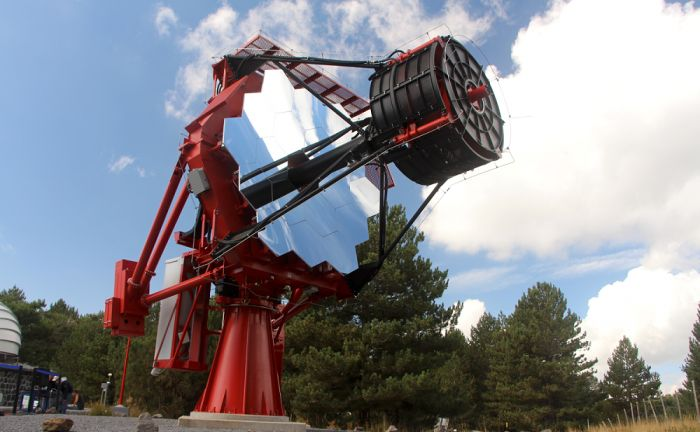
\includegraphics[width=.9\textwidth]{images/sst.jpg}
		\caption{An illustration of the Small Sized Telescope (SST) with its
		two mirrors.
		The dual-mirror Schwarzschild-Couder setup includes mirrors of
		\SI{4.3}{\meter} and \SI{1.8}{\meter} diameter.
		The image can be found at the official CTA-website \cite{cta_web}.}
		\label{fig:sst}
\end{figure}
\chapter{machine learning, statistic, estimations}\label{ml}

cta datenmengen, vergleich auch ein apar andere experimente um größenordnung darzustellen, zitieren!

Given these enormous amounts of data, it comes as no surprise that
various data reduction techniques are getting applied in many modern
physics experiments (citation needed!).
Various machine learning models have proven to be
quite sucessfull in solving classification and
regression problems (citation needed).
This thesis focusses on using random forests to
perform gamma/hadron separation, energy estimation, and
source position estimation.
As these are rather sophisticated algorithms, I will
give a short introduction into the basics of machine learning.

\section{Supervised learning}
In the task of supervised machine learning a model is trained on a
dataset, that full information is given on. The trained model
can then later be used to estimate values from a dataset, which
lacks our needed information. In machine learning we differentiate
the columns of our dataset in a set of \textbf{input} variables $X$ and
a set of \textbf{output} variables $y$. The naming convention for
these sets follows the convention of scikit-learn
\cite{scikit-learn}, \cite{sklearn_api}, a python package for
machine learning algorithm, which will be used to implement the models later on.
Other terminologies for the two feature sets include
predictors or independent variables for the input, and
responses or dependent variables for the output.

\subsection{Classification}
In (supervised) classification tasks, we want to predict the membership to
a set of predefined classes. The possible solutions for $y$
are from a discrete set of qualitative values (???).
A common example for a classification problem is an e-mail spam filter,
where mails get categorized in at least two categories based
on their content and meta data \cite{DBLP:journals/corr/cs-CL-0006013}.

The simplest and most popular case of classification problems
is \textbf{binary classification} \cite{sokolova2009systematic}.
In this case only two distinct
classes exist, which is all we will need for signal/background-separation.
For binary classification we can define a set of measures
to define the quality of our prediction, starting with the confusion matrix.
These follow the notation and description of \cite{sokolova2009systematic}.

\begin{center}
    \begin{tabular}{ | l | l | l |}
    True label & Predicted as $pos$ & Predicted as $neg$ \\ \hline
    $pos$ & true positive ($tp$) & false negative ($fn$) \\ \hline
    $neg$ & false positive ($fp$) & true negative ($tn$) \\ \hline
    \end{tabular}
    \caption{Confusion matrix for a binary classification task with
    the two labels $pos$ and $neg$.}
\end{center}

An ideal classification would result in
\begin{equation*}
  fp = fn = 0.
\end{equation*}
Based on the confusion matrix, multiple measures exist.
Some of the more common ones are:

\begin{center}
    \begin{tabular}{ | l | l | l |}
    Measure & Formula as $pos$ & Evaluation Focus \\ \hline
    Accuracy & \frac{tp+tn}{tp+fn+fp+tn} & Overall effectiveness of a classifier \\ \hline
    Precision & \frac{tp}{tp+fp} & Class agreement of the data labels with the positive labels given by the classifier \\ \hline
    Recall/Sensitivity & \frac{tp}{tp+fn} & Effectiveness of a classifier to identify positive labels \\ \hline
    F-score & \frac{(\beta^2+1)tp}{(\beta^2+1)tp+\beta^2fn+fp} & Relations between data’s positive labels and those given by a classifier \\ \hline
    Specificity & \frac{tn}{fp+tn} & How effectively a classifier identifies negative labels \\ \hline
    AUC & \frac{1}{2}(\frac{tp}{tp+fn}+\frac{tn}{fp+tn}) & Classifier’s ability to avoid false classification \\ \hline
    \end{tabular}
    \caption{Confusion matrix for a binary classification task with
    the two labels $pos$ and $neg$.}
\end{center}

A model that performs classification on data is often referred to as
classifier.

\subsection{Regression}
In contrast to classification, regression refers to predicting
a continous output.
LINEAR LEAST SQUARES
BEISPIELE FÜR KOMPLEXERE METHODEN
METRIKEN ZUR BEURTEILUNG (WIE IN DER KLASSIFIZIERUNG)


\subsection{Learning as optimization problem}
kommt quasi aus der regression raus -> SSE minimiert
\subsection{Bias and variance, validation?, R2-Score}



cart erwähnen? sklearn macht cart
relativer vs absoluter fehler (-> log energie)
\section{Decision trees and random forests}
Methods based on Decision Trees work by recursively partitioning
the parameter space until the output values can easily be estimated
in the respective regions of the parameter space.
Tree-based methods can be applied to both classification and regression tasks.

\subsection{Decision trees, parameter estimation, gini?}
A simple Decision Tree can look like shown in figure \ref{fig:03_tree}.

\begin{figure}
  \centering
  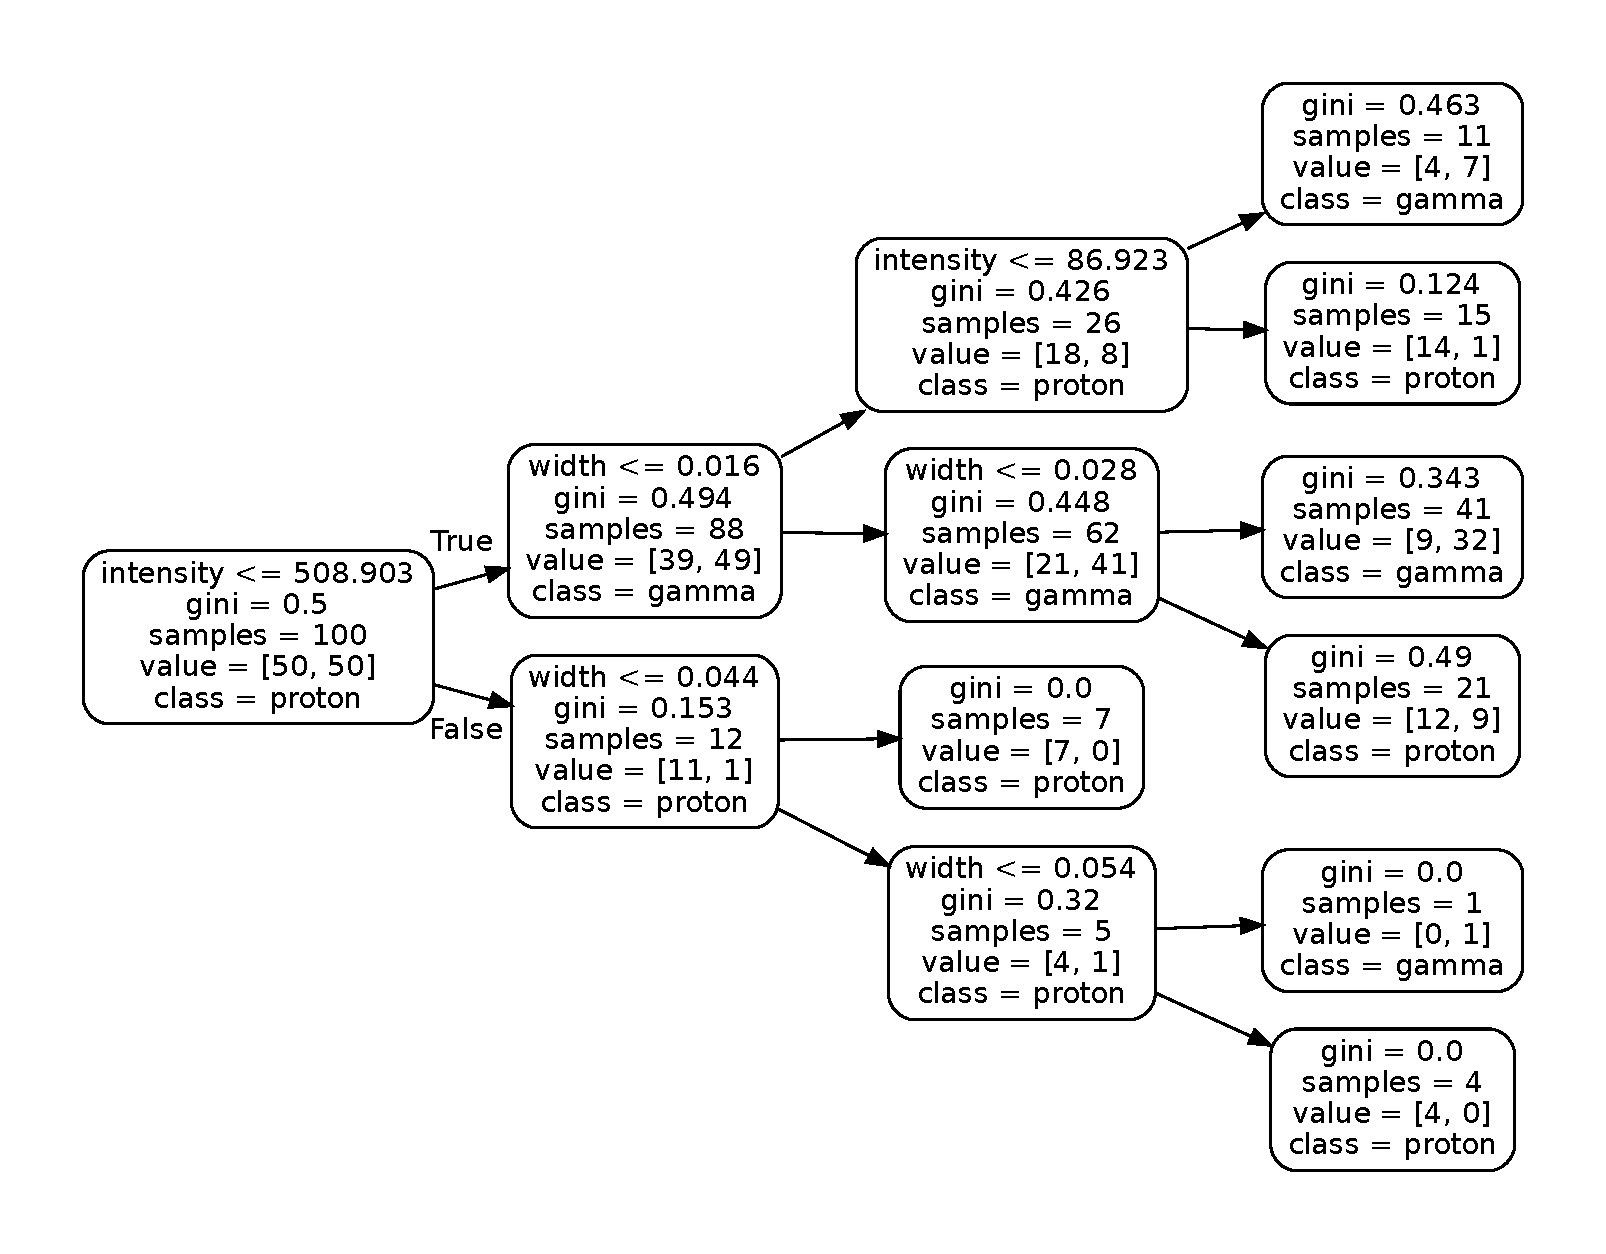
\includegraphics[width=0.7\textwidth]{Plots/decision_tree.pdf}
  \caption{Sample decision tree used to classify flowers in
  the iris dataset \cite{fisher1936use} \cite{sklearn}.}
  \label{fig:03_tree}
\end{figure}

Starting from the root node, a binary split is performed to
split up the data. For each split additional splits are performed
until a stopping criterion is reached.
How to choose the optimal split is defined as minimizing a
pre-defined measure. For classification tasks often used measures
are the above used gini coefficient (zitat) and the
cross-entropy (zitat).

indizes erklären!
\begin{equation}
  \text{Gini coefficient: } \\
  \text{Cross-entropy: }
  \label{eq:03_gini_ce}
\end{equation}

A stopping criterion can be defined as the measure reaching zero or
falling under a defined threshold.

For regression tasks the mean squared error or mean absolute error
are used and the same principles apply.
\begin{equation}
  \text{mse: } \\
  \text{mae: }
  \label{eq:03_mse_mae}
\end{equation}

To avoid overly complex trees, which would result in both high memory
consumption and potential overfitting on data, decision trees are often
limited to a certain depth, reducing the complexity of the model.
While decision trees have the benefit of providing
easily interpretable, low bias models there are some drawbacks to this
approach, namely \cite[hastie2017springer]:
\begin{itemize}
  \item{Instability, high variance}
  \item{Lack of Smoothness}
  \item{Difficulty in Capturing Additive Structure}.
\end{itemize}

Approaches to reducing these problems include
boosting \cite{freund1997decision} and Random Forests \cite{Breiman2001}.

\subsection{Random forests}
The main idea behind random forests is to use multiple, independent
decision trees to suppress the problems single trees have, while
keeping their advantages. For this to work, the individual trees need
need not to be correlated. Consequently the trees cannot all
be constructed the same way. Instead each tree performs splits
regarding a random subset of all available variables.
The Prediction of the random forest is then either the average of
the single predictions in case of a regression task or
the majority vote of the single predictions in case of classification.

Formel 15.1 aus hastie erklären

Random forests have become one of the standard algorithms
in our data analysis, because according to our
experience and \cite{hastie2017springer} they tend to
not overfit (as long as the individual trees have no or little bias)
and generally perform decent without a lot of manual tuning.


\section{mean estimation stuff, outlier resistance, unsupervised? clusters?}
warum robuste schätzer?
verwendete algorithmen

\chapter{analysis}\label{analysis}

ToDo:
\begin{enumerate}[nosep]
    \item Datenformat Input, verwendete Daten, Worte zu Simulation, trainingsdaten
    \item Preprocessing - Schritte erklären
    \item Datenformat Output Preprocessing
    \item ...
    \item Anwendung Random Forests mono, disp erklären anhand hillas parameter
    \item Anwendung Stereo (Random forest, stabile Mittelwertverfahren -alle erklären)
    \item Signifikanzkurve
\end{enumerate}

\section{preprocessing}
% configuration in appendix! + algorithmen beim prep

\subsection{Monte Carlo Data}
At the lowest level our observed data consists of uncalibrated waveforms 
in the camera pixels.
prod3b stuff kurz anreißen
wahl des arrays!

\subsection{Reconstruction on telescope level+hillas reconstructor}
% definition datenlevel
- calibration
- cleaning
- hillas parameters 
- telescope level
- tabellen der features bei runs/arrays/telescopes

To be able to apply high-level analysis methods, the initial data 
needs to be reduced and preprocessed substantially.

To specify a specific event, we will identificate an event based on 
three layers:
\begin{enumerate}
    \item{Run-Id: This gives us non-event-specific information about the monte carlo run, e.g.
    spectral\_index, particle injection height, ...}
    \item{Array-event-id: Any shower that triggered the array is considered to be an array event.
    Array-level features consist of general event information (e.g. number of triggered telescopes, average internsity)
    reconstructed features of the primary particle (energy, source position, ...) and the 
    event specific monte carlo information to compare these features against.}
    \item{Telescope-event-id: This specifies how a specific telescope has seen the shower and
    contains information about the telescope itself (e.g.focal length). Telescope-level features 
    describe the camera image, amongst other things via the hillas-parameters(cite stuff)}
\end{enumerate}


In the following we will 
distinguish between "array-events" and "telescope-events" when describing the reconstruction methods.

Processing of the Simtel-files is done with the aforementioned ctapipe, starting with 
the calibration of the (array) event. This performs an integration of the waveforms in 
each pixel of the camera of a triggered telescope. Inside ctapipe the initial data is referred to as R1
and the reuslting data as dl1. The resulting images get cleaned with a tailcuts approach before they are
used to calculate image features, such as the hillas parameters.

Hier part über hillas params mit den bildern! erklären wieso und so
\begin{figure}
    \begin{subfigure}{0.3\textwidth}
        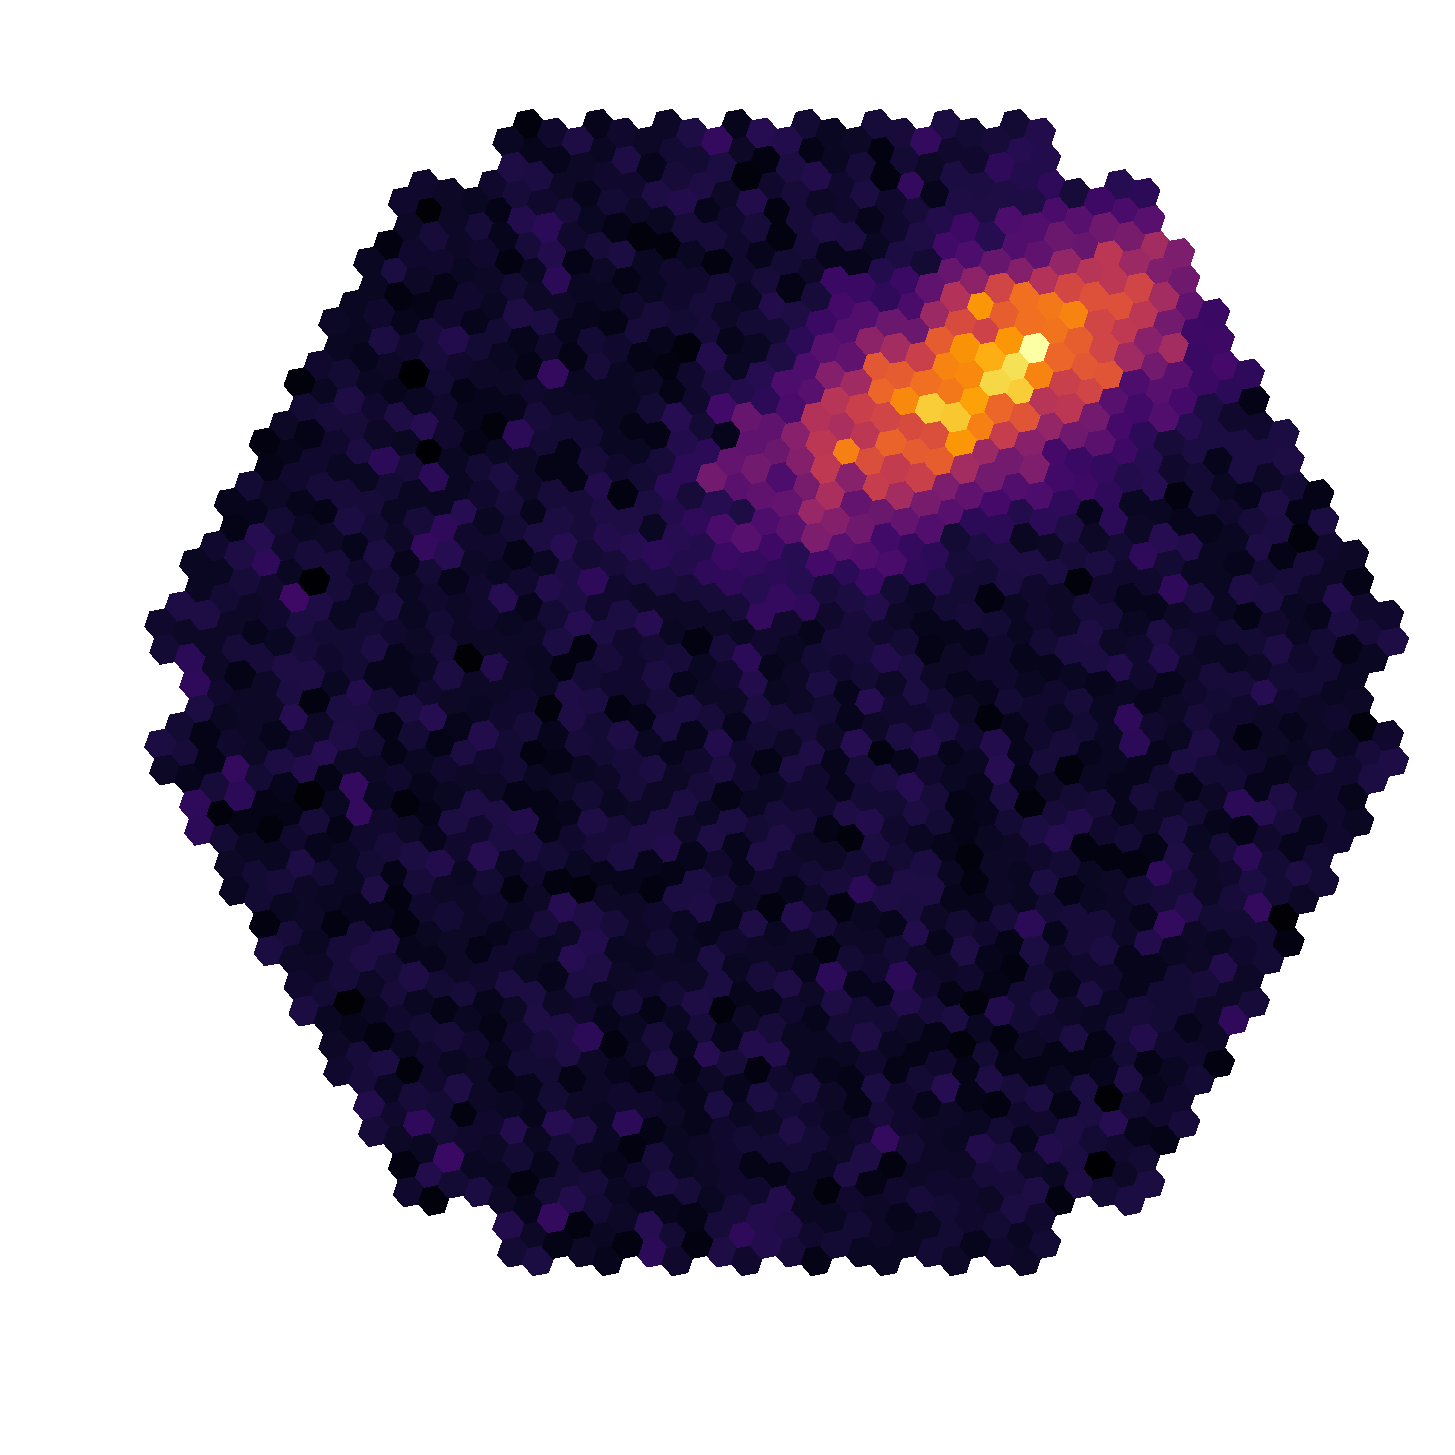
\includegraphics[width=0.9\linewidth]{Plots/hillas_raw.pdf} 
        %\caption{Caption1}
        \label{fig:shower_image_raw}
    \end{subfigure}
    \begin{subfigure}{0.3\textwidth}
        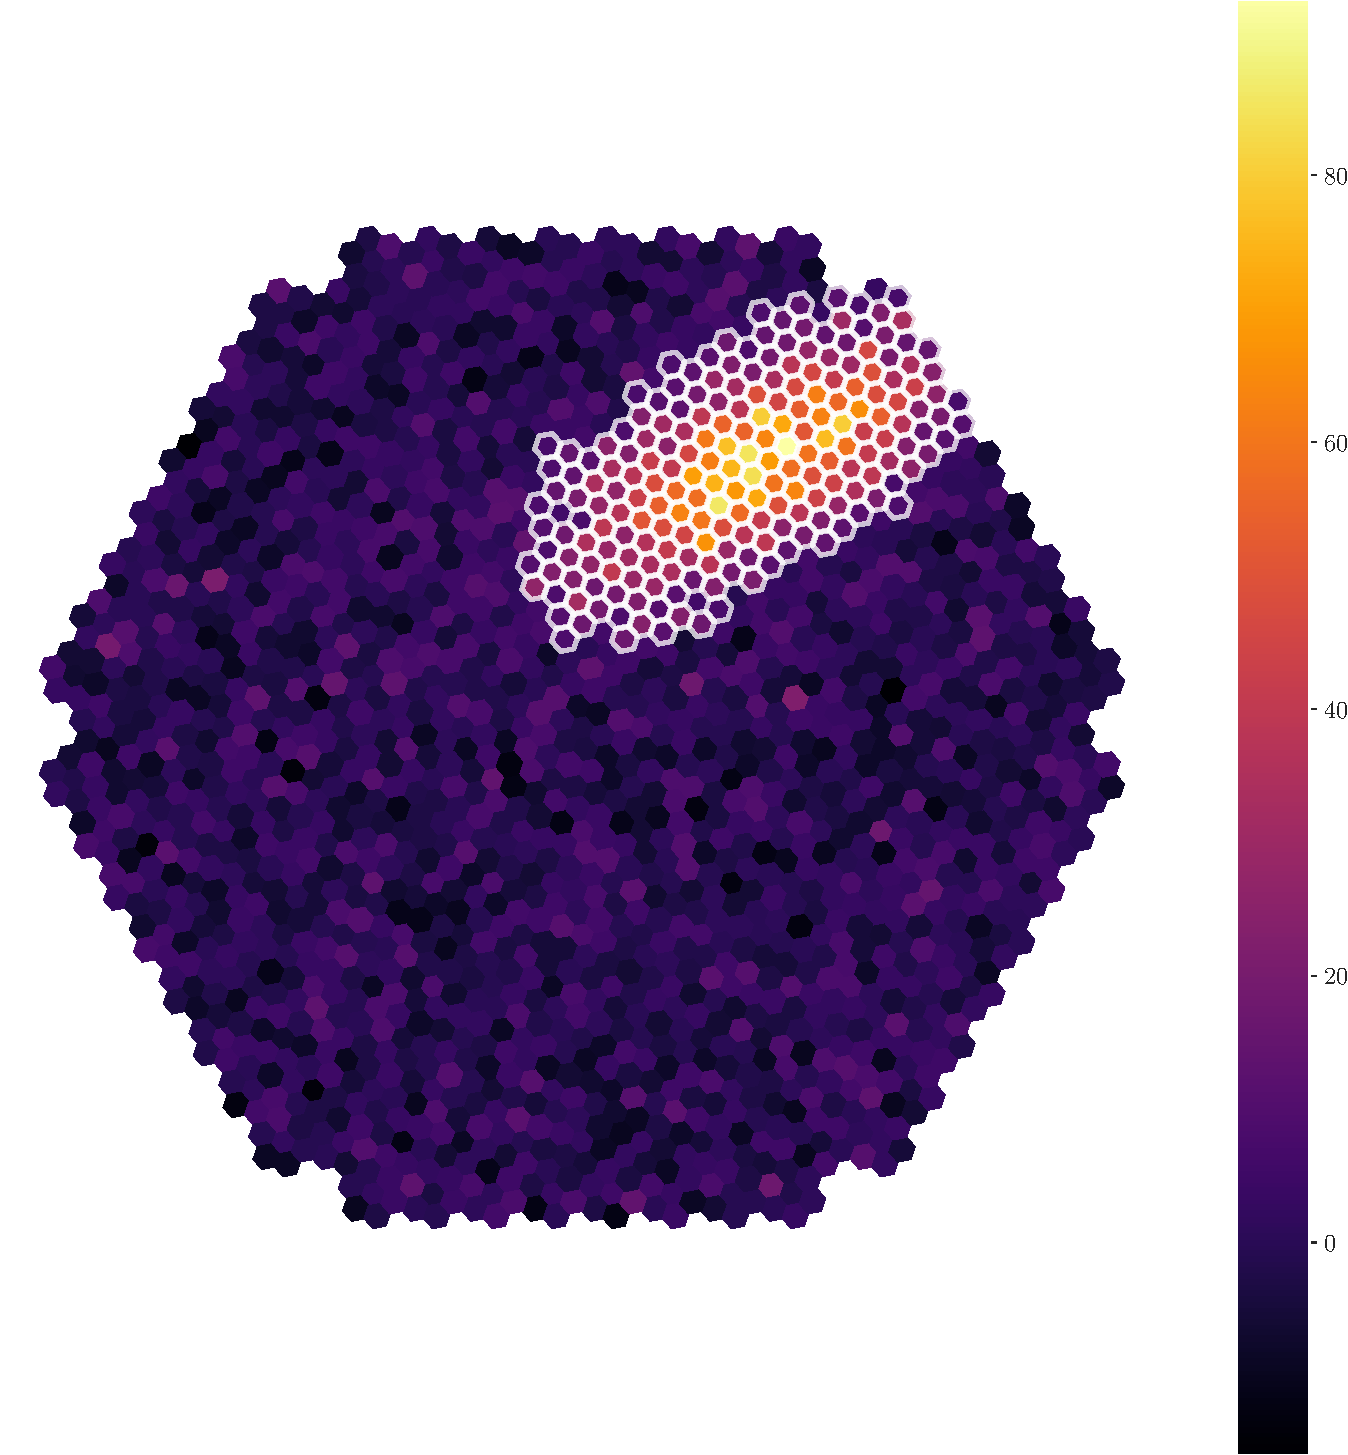
\includegraphics[width=0.9\linewidth]{Plots/hillas_cleaned.pdf}
        %\caption{Caption 2}
        \label{fig:shower_image_cleaned}
    \end{subfigure}
    \begin{subfigure}{0.3\textwidth}
        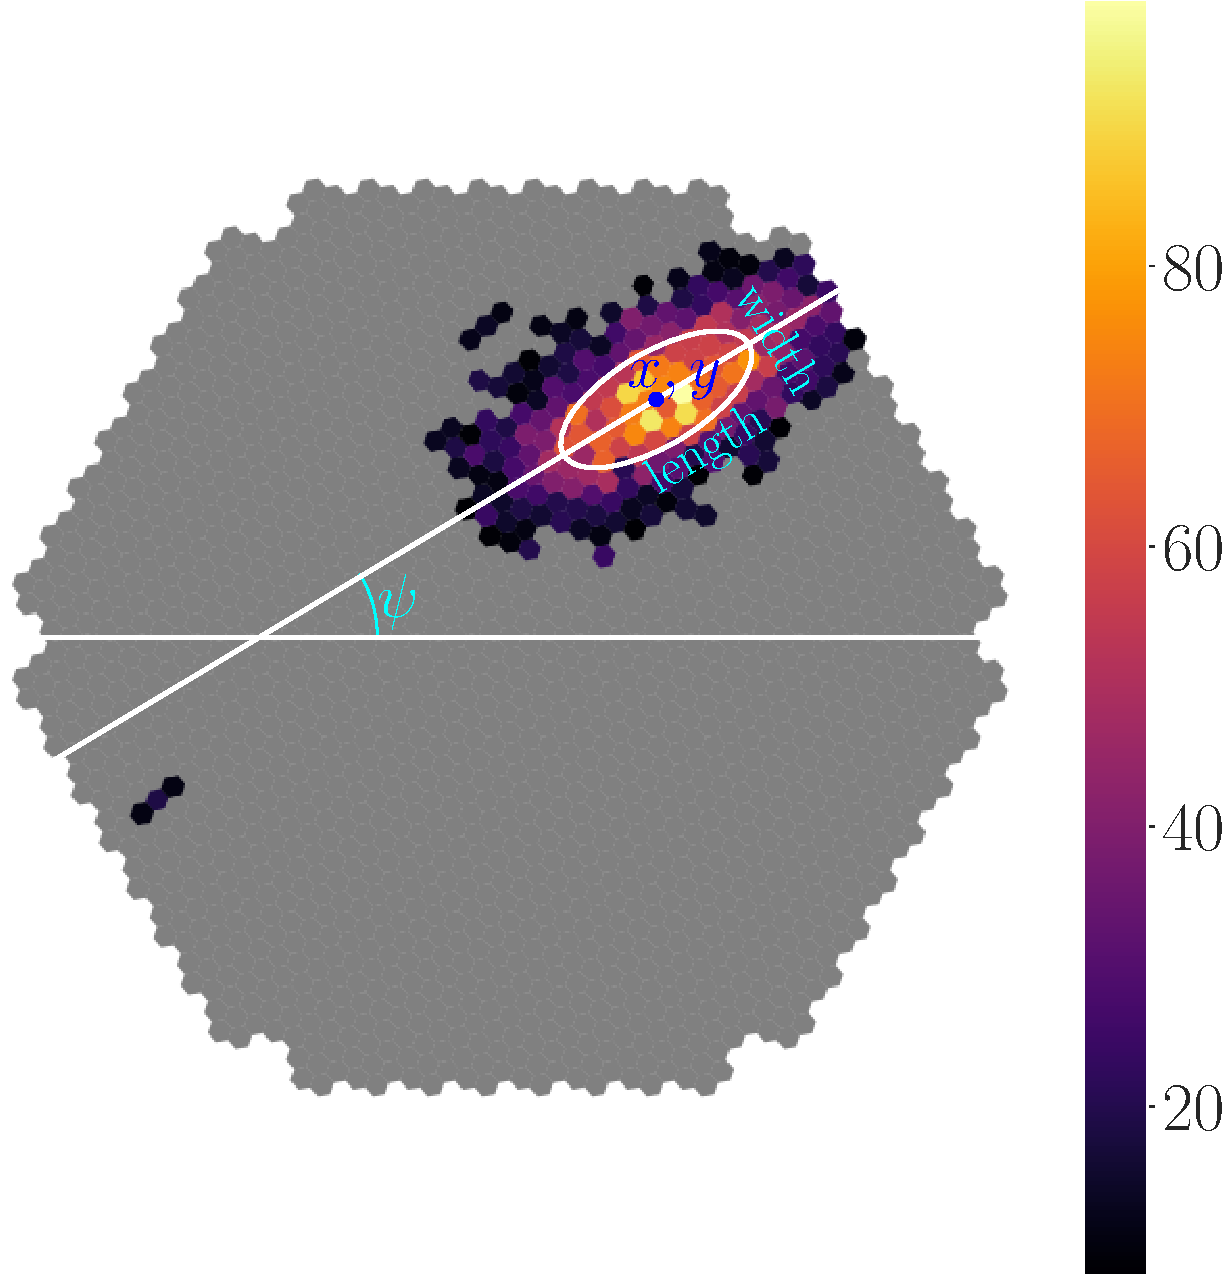
\includegraphics[width=0.9\linewidth]{Plots/hillas_cleaned_params.pdf} 
        %\caption{Caption1}
        \label{fig:hillas_parameters_only}
    \end{subfigure}
    \caption{Illustration of a simulated gamma shower captured with the LST-telescope.
        The left figure shows the image after applied waveform-extraction but before
        the cleaning step. The right figure shows the image after the cleaning has been applied
        and non-selected pixels have been discarded.}
    \label{fig:shower_image}
\end{figure}

In addition to the original hillas parameters, the concentration, number of islands and timing parameters
get calculated.
Concentration refers to the intensity captured in the brightest pixel or the cog relative to 
the total intensity in the image.
An island is considered a connected cluster of pixels. In an ideal gamma shower image, only one island
is expected, although this is highly dependend on the applied cleaning.
Timing parameters are the second momenta of the distribution of the relative peak arrival times
in each pixel, which can be derived form the waveforms.

All these features get used in the machine learning algorithms at later stages.

\subsection{Hillas reconstructor}  % we dont seperate between 0 and 1 right?
After the image processing of each associated telescope image has been finished,
the predictions of our "baseline" source position estimator get calculated.
This algorithm is referred to as HillasReconstructor inside ctapipe, because 
it works based on the hillas parametrisations of the images.
For each triggered telescope, a 2D-plane is drawn based on the main shower 
axis and the telescope orientation. These planes intersect and 
the weighted average of all intersections gives the 
direction of the shower origin (cite code or paper).

%% input ausgelagerten hillas tikz kram

Since this method inherently requires a stereoscopic experiment
and multiple triggered telescopes, it will not work for a single telescope.
From earlier studies (kram zitieren, zb kai), it is expected
that this method works best with an event multiplicity 
(number of triggered telescopes) \geq 3 with higher multiplicity
leading to better results.

\section{Machine Learning, dl3?}
High level analysis of the preprocessed data is based on the use of
the aict-tools \cite{aict-tools} package which itself is based on
sklearn \cite{sklearn_api} for the machine learning algorithms.
The algorithm of choice is the Random Forest algorithm
as it is well suited for the use with tabluar data and tends to rarely overfit
(citation needed).
Seperate models are trained for the tasks of signal/background
separation, signal energy estimation and signal source position
reconstruction.
The aict-tools have originally been developed for the FACT-experiment
(citation needed) which is a single IACT. For this reason
adaptions had to be made to perform a stereoscopic analysis.


\subsection{g/h sep}
For the task of gamma/hadron separation a random forest can be trained
using either only monoscopic information or also using array-level
information from earlier reconstruction steps.
This generally improves the accuracy by a few percent points.
The single telescope predictions can be combined by
simple functions such as the mean or median of the
single predictions to provide a prediction for the complete
array-event.
% features und kram


% \section{energy estimation}
% Energy estimation can be performed in the same way as the gamma/hadron
% separation. For this task there has been earlier work indicating
% the usefulness of a second machine learning model trained
% on the predictions of the first telesope-level model
% \cite{ba-lars}.

% I am thus going to present results based on either calculating the mean
% of the telescope level predictions and using a second random forest
% to improve the array level prediction.

\subsection{source position}
\label{sec:source_position}
Given the source position in the camera frame the source position
on the sky can be calculated with coordinate transformations if
the position, pointing and optical properties of the
telescope are known.
In general the true source position in the camera frame is assumed to be
different from the center of gravity of the shower ellipse
but located somewhere along the main shower axis.
This assumption seems to hold decently well, .... zitat.

The position on the shower axis can be estimated based on 
the hillas parameters and other image features.
This method is known as the DISP-method in the
literature (citation needed). The general idea 
can be seen in figure \ref{fig:disp}.

\begin{figure}
    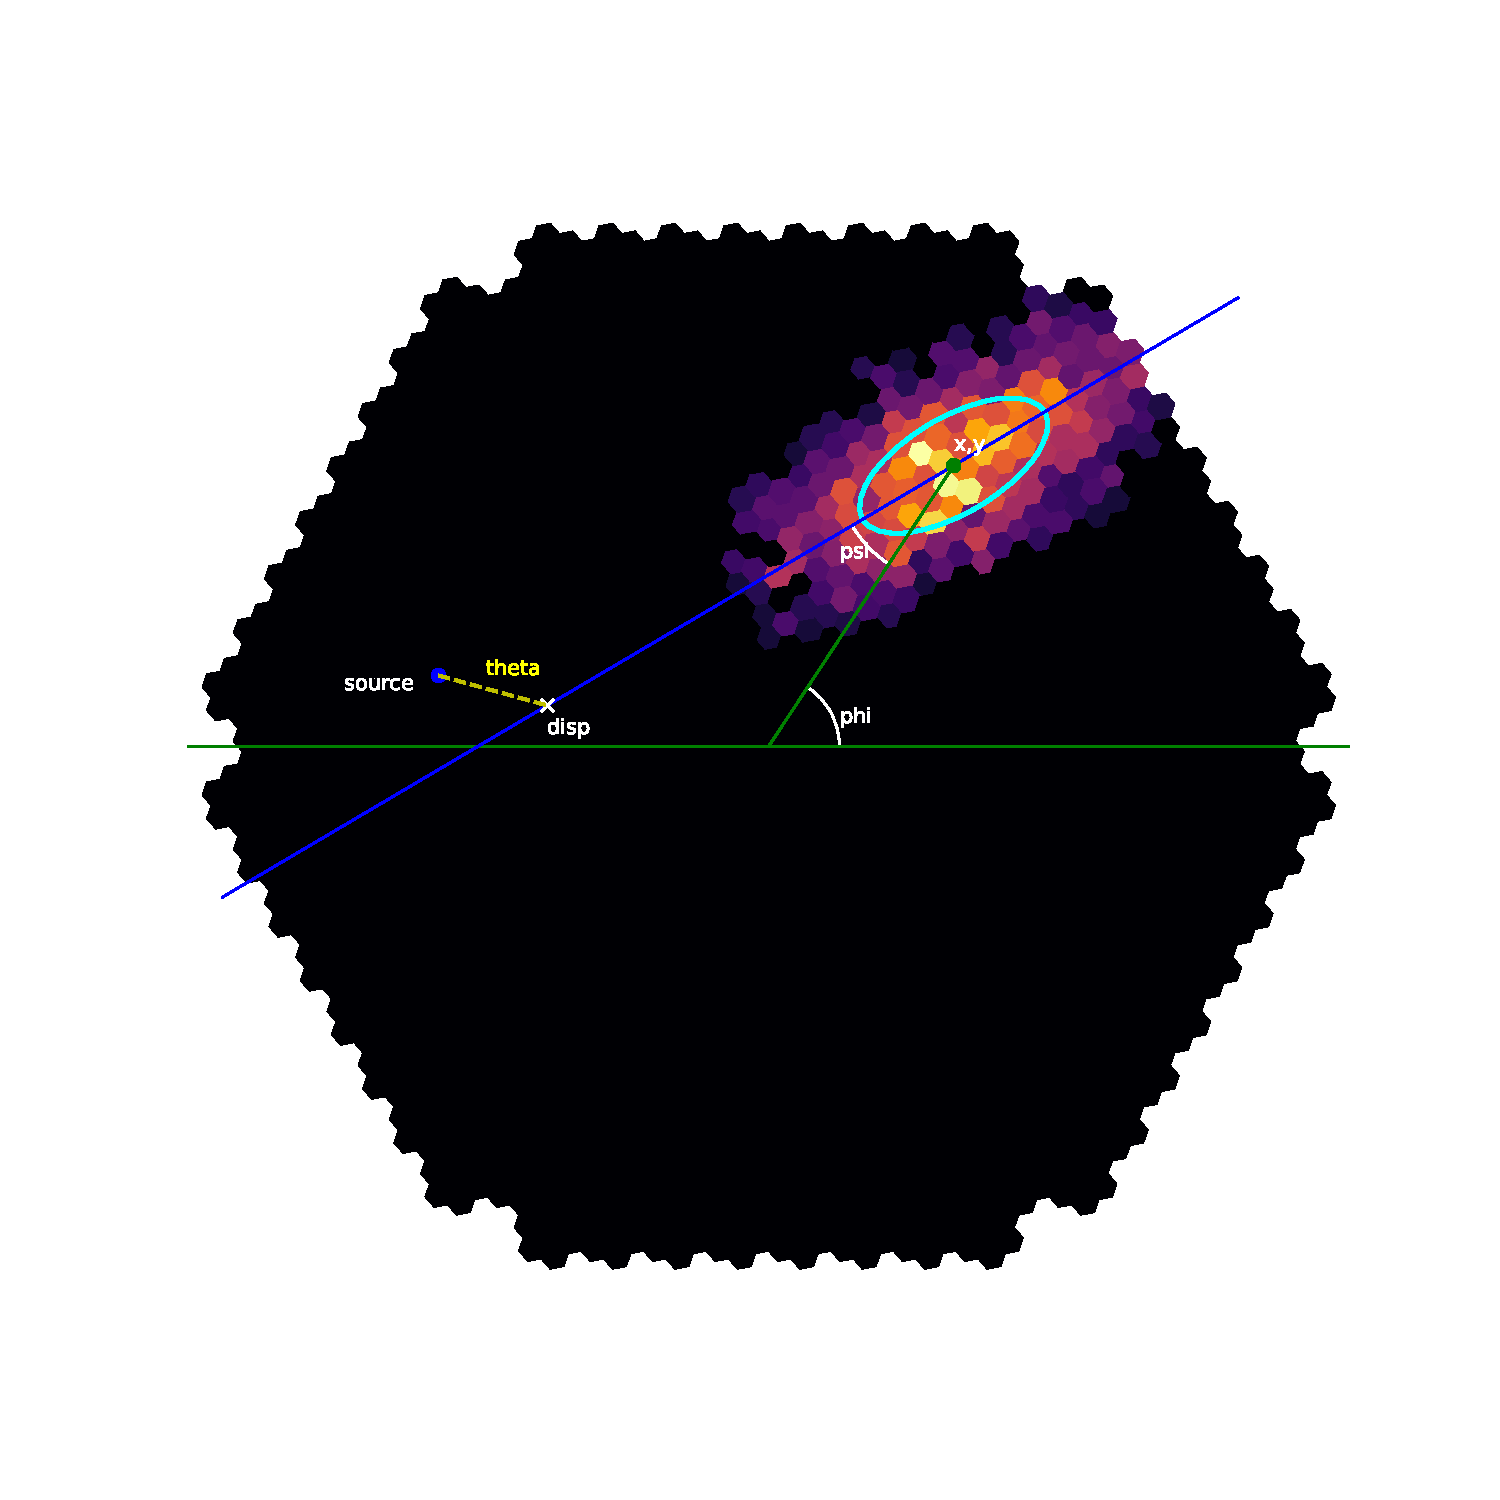
\includegraphics[width=0.9\linewidth]{Plots/hillas_complete.pdf}
    \caption{Illustration of monoscopic source position reconstruction making use of 
        the Hillas-Parameters and the DISP-method as explained in section \ref{sec:source_position}.
        The left figure has the hillas ellipse and parameters drawn onto our previously cleaned sample shower.
        The right figure estimates a source Position in the Camera frame.}
    \label{fig:disp}
\end{figure}

With the DISP-method the estimated distance between the source
position and the center of gravity of the hillas ellipse gets calculated
based on the form of the ellipse, timing information and potentially
more features.
This can be done analitically, via lookup-tables or with machine learning.
At this point the reconstructed source position
is fixed at two points at the main shower axis, see figure \ref{fig:disp_amb}


\begin{figure}
    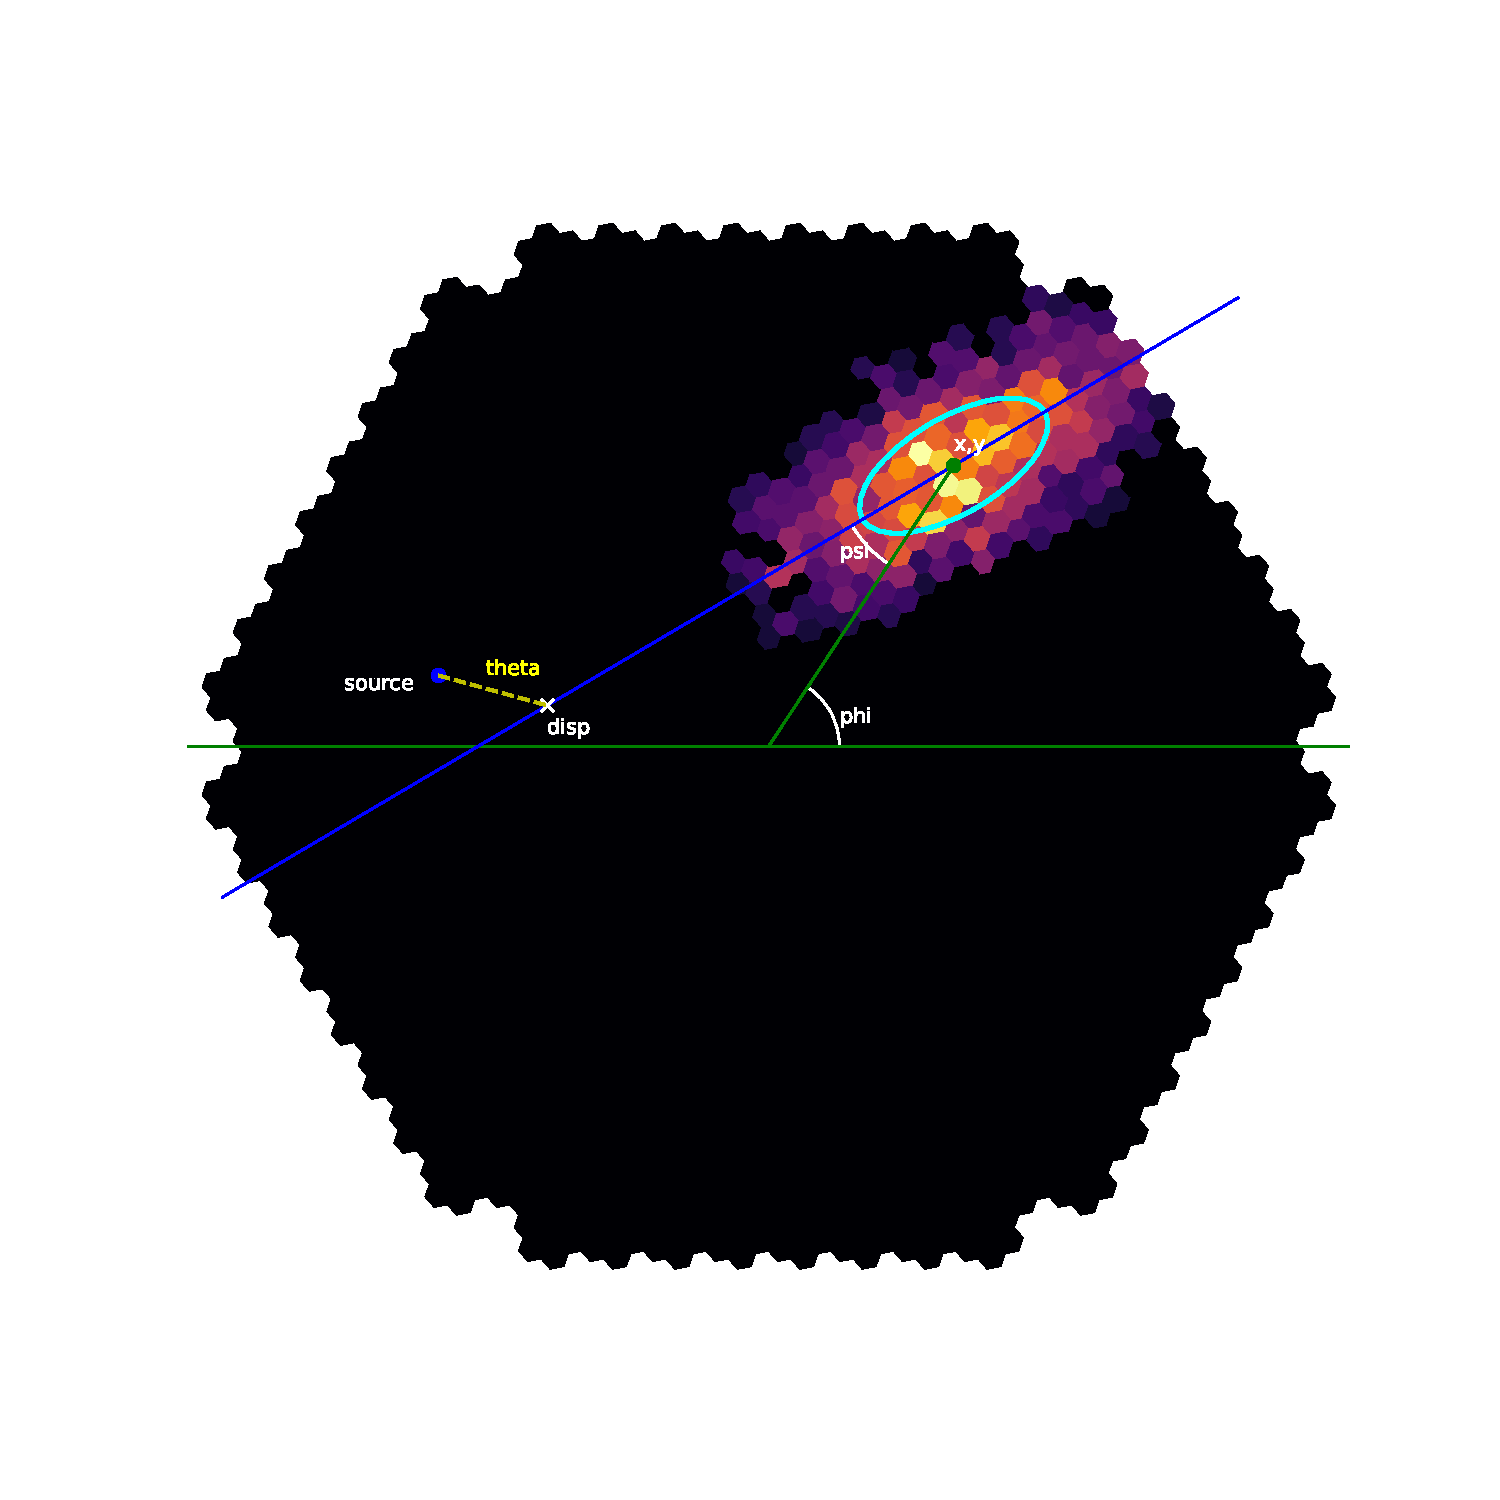
\includegraphics[width=0.9\linewidth]{Plots/hillas_complete.pdf}
    \caption{Wrong pic!}
    \label{fig:disp_amb}
\end{figure}


The remaining task then consists of finding the correct one of these
two points. If there is no stereoscopic information available,
a choice can be made based on the image features again.
In FACT-analyses a second random forest is trained for this
specific purpose, usually yielding an accuracy around 70-80\% (citation).
This is called SIGN-prediction, interpreting the two possible sides
as +-1, allowing for binary classification.
In the case of the MAGIC-telescopes the ambiguity does not
get resolved until the individual results get combined
on the stereo level. The choice of the correct
pair out of the four reconstructed positions can be done either
by calculating the crossing point of both main shower axises
or by calculating the pairwise distances between the positions (citation).


These methods are illustrated in figure \ref{fig:disp_magic}


\begin{figure}
    \begin{subfigure}{0.3\textwidth}
        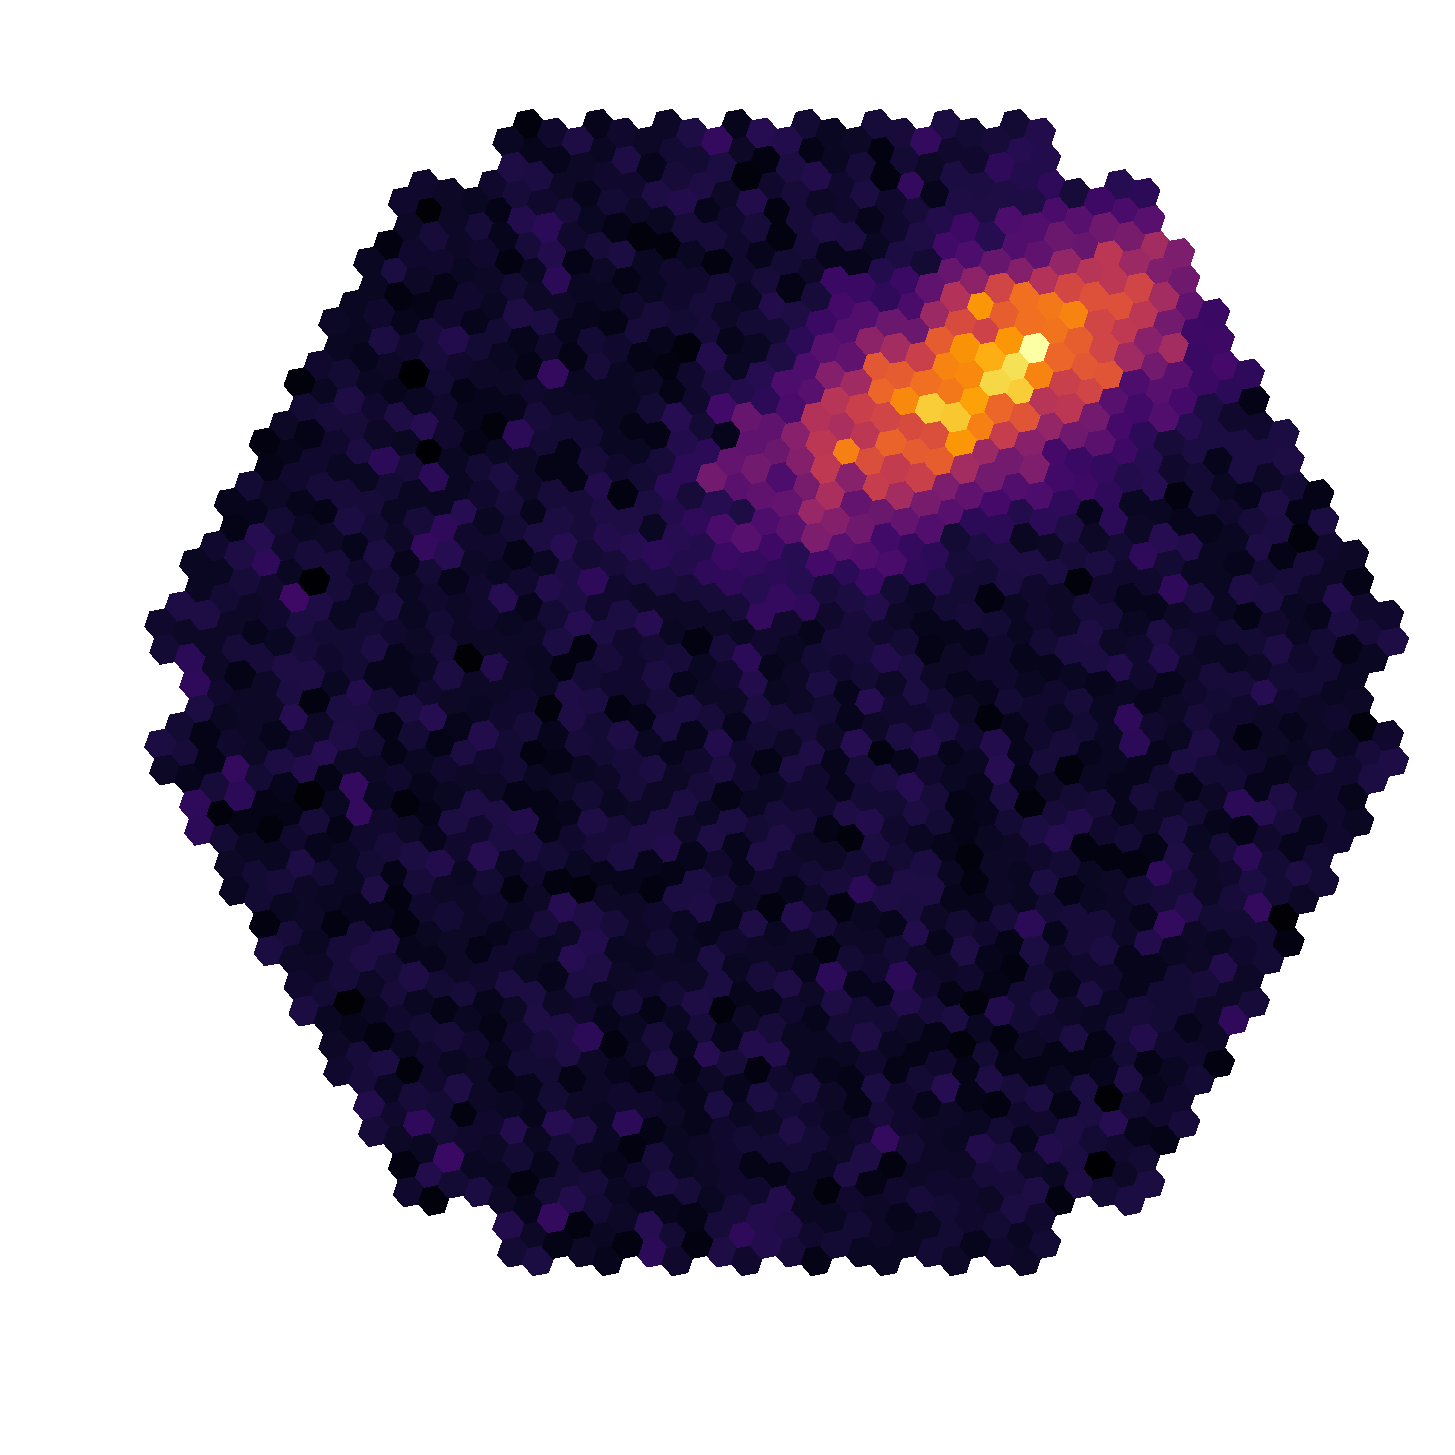
\includegraphics[width=0.9\linewidth]{Plots/hillas_raw.pdf} 
        %\caption{Caption1}
        \label{fig:3}
    \end{subfigure}
    \begin{subfigure}{0.3\textwidth}
        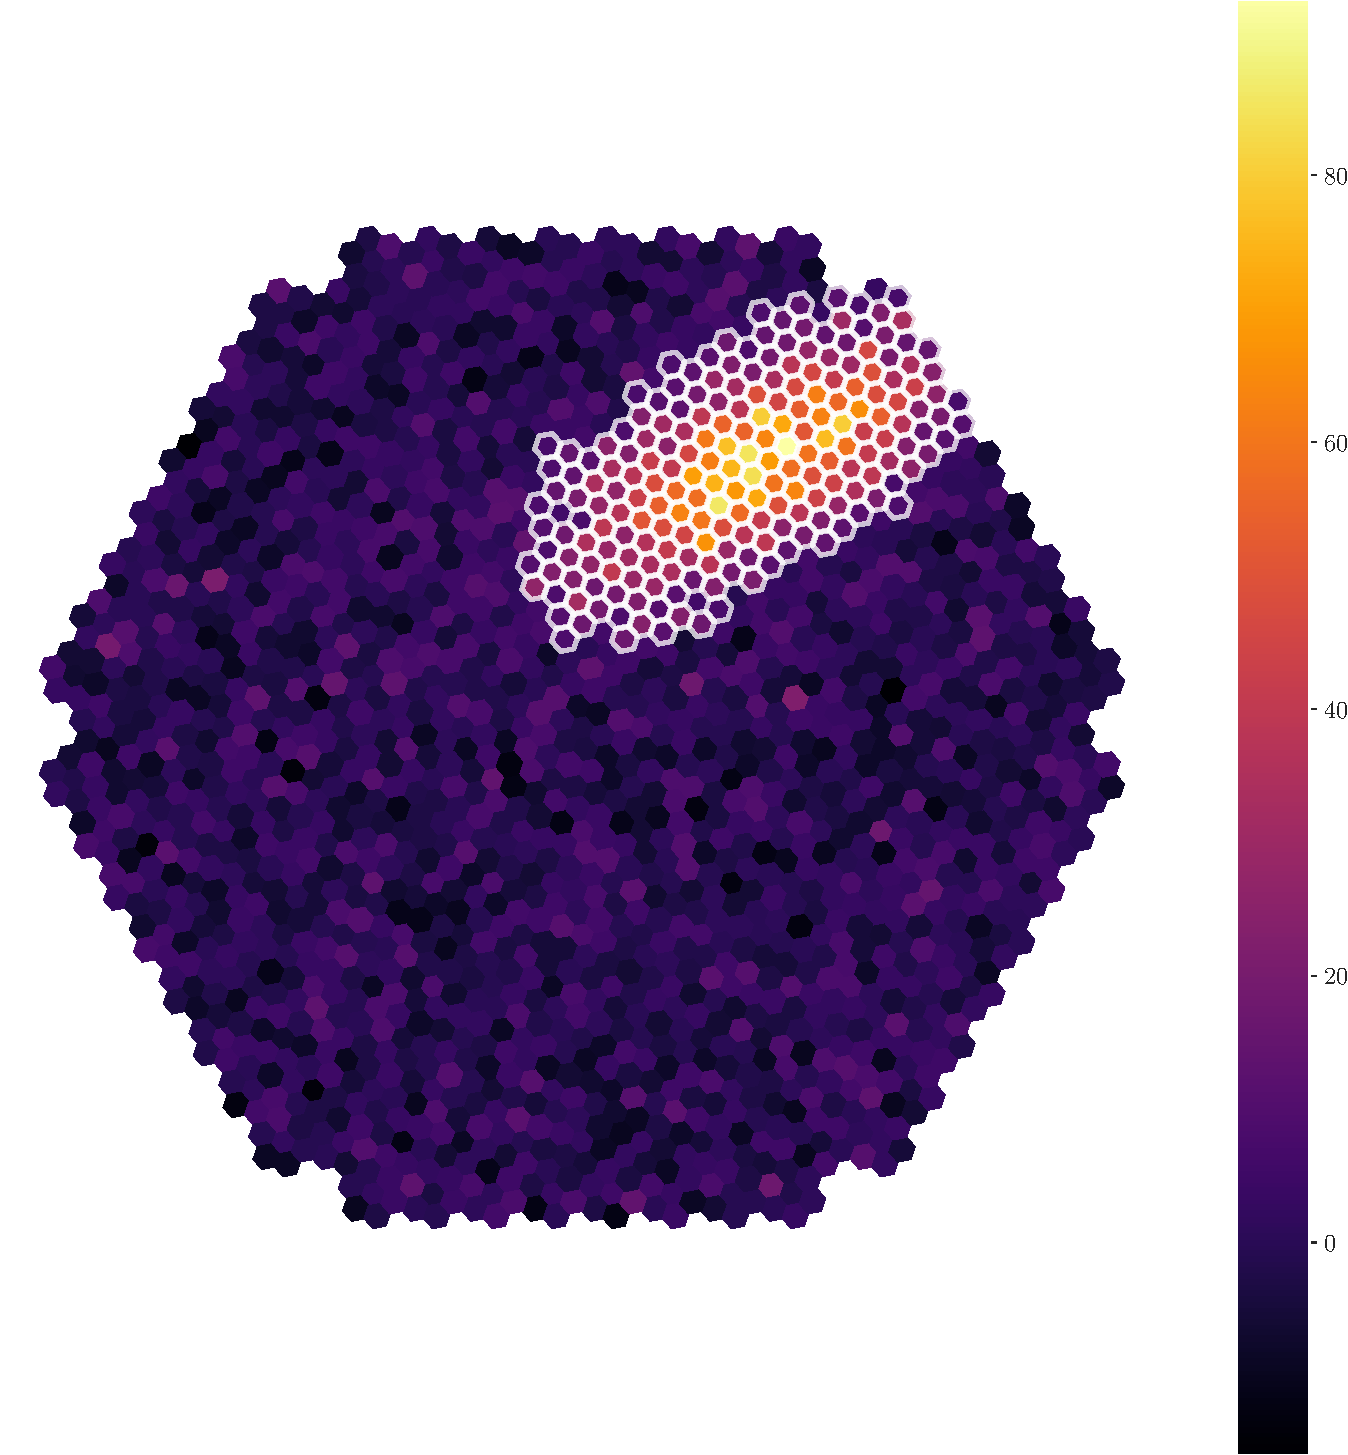
\includegraphics[width=0.9\linewidth]{Plots/hillas_cleaned.pdf}
        %\caption{Caption 2}
        \label{fig:2}
    \end{subfigure}
    \begin{subfigure}{0.3\textwidth}
        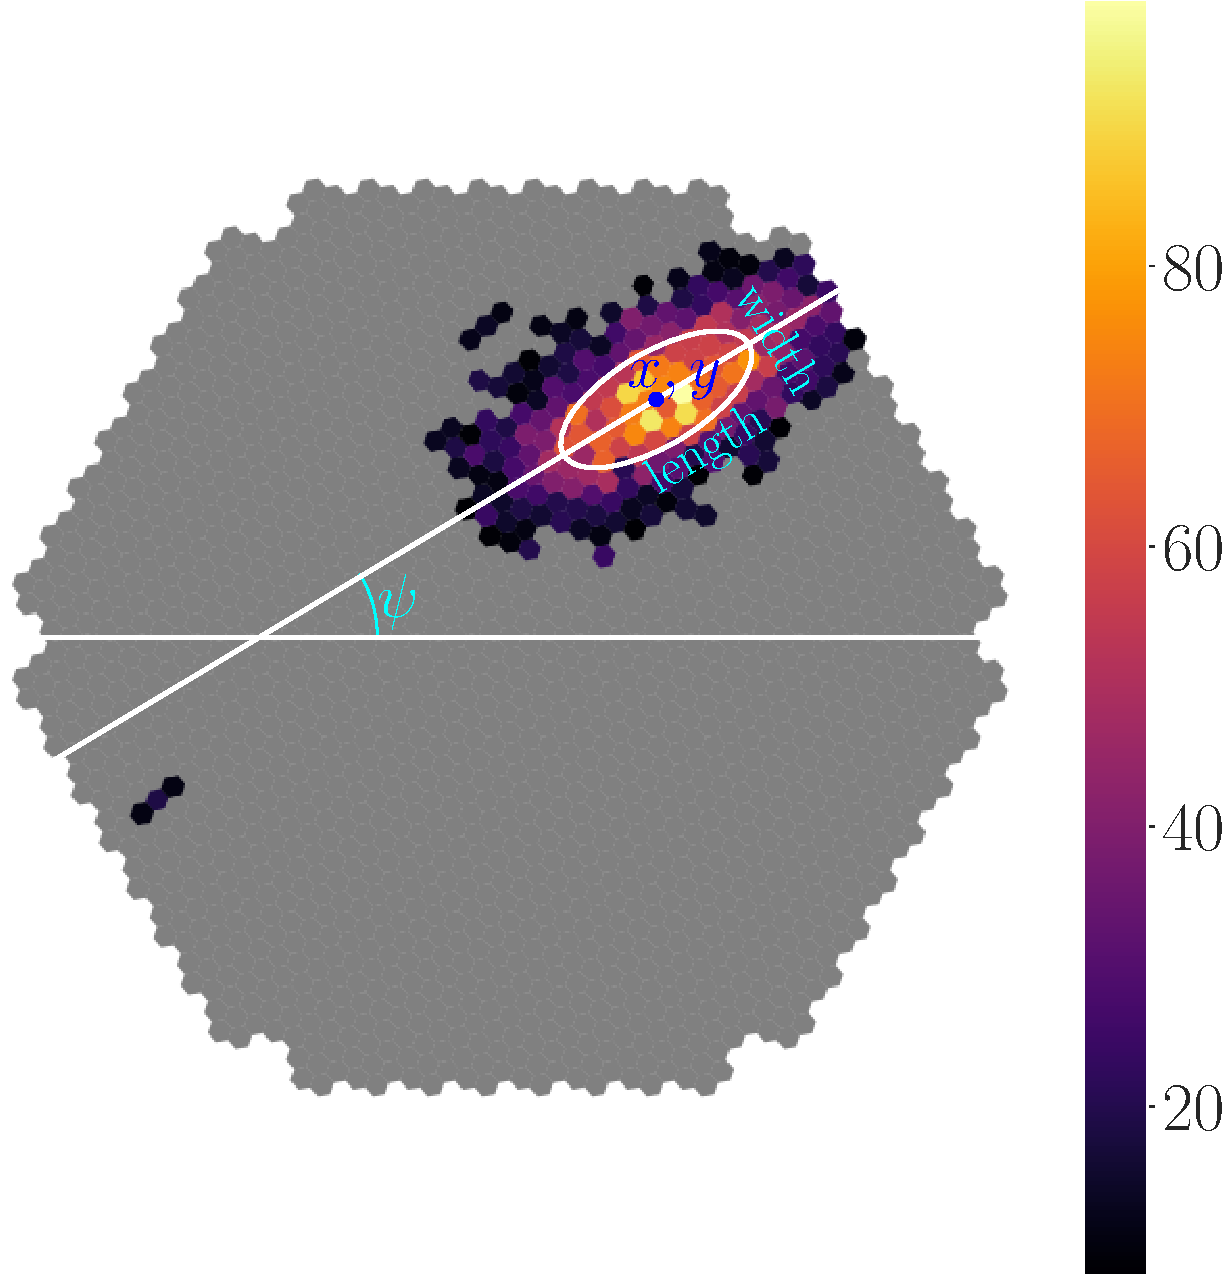
\includegraphics[width=0.9\linewidth]{Plots/hillas_cleaned_params.pdf} 
        %\caption{Caption1}
        \label{fig:1}
    \end{subfigure}
    \caption{wrong pics}
    \label{fig:disp_magic}
\end{figure}





\section{Analysed Data}
\subsection{Corsika Simulation}
\subsection{Training, Testing, mismatches und so, weniger telescope daten bei weniger teleskopen! duh... aber wichtig für statistik.}

\chapter{results}\label{results}


\section{ghsep}\label{ghsep}

The random forest for the gamma-/hadron-separation gets trained on 
\num{5753708} diffuse gamma events and \num{6035652} diffuse proton events with a 5-fold cross-validation.
We define the class gamma to be of value 1 and protons of value 0.
The random forest predicts a "gammaness" between 0 and 1.
With these parameters, the distribution of the predicted gammaness
is illustrated in figure \ref{fig:gh_sep}.

\begin{figure}
    \centering
    \includegraphics[page=2, width=.8\textwidth]{../analysis/plots/cross_val_sep_perf_plot.pdf}
    \caption{Distribution of the predicted gammaness on the cross-validated training data.
	    The two populations (Proton and Gamma, marked in blue and orange), can be separated 
	    to a certain degree. Over $\approx \num{0.5}$ the preidctions for protons decrease rapidly.
        A perfect prediction (AUC=1) would show no overlap between the distributions.}
    \label{fig:gh_sep}
\end{figure}

The ROC-curve is shown in figure \ref{fig:gh_roc}, with the model achieving an AUC of 
\num{0.835}.


\begin{figure}
    \centering
    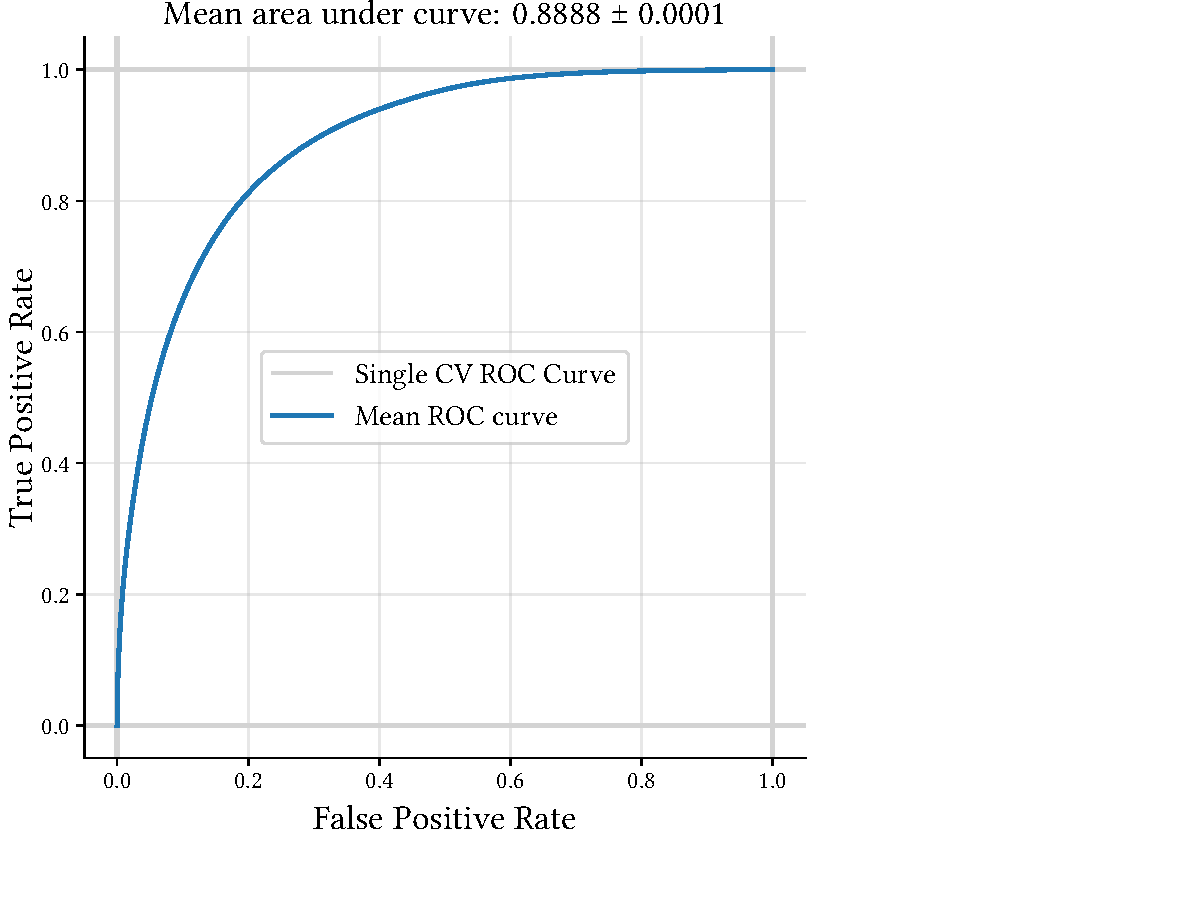
\includegraphics[page=1, width=.8\textwidth]{../analysis/plots/cross_val_sep_perf_plot.pdf}
    \caption{ROC-curve for the gamma/hadron separation on the cross validated training set 
    consisting of \num{6035652} proton events and \num{5753708} diffuse gamma events in total.
    The five ROC-curves from the individual cross validation steps show almost no deviation.}
    \label{fig:gh_roc}
\end{figure}


The feature importance, as calculated via sklearn, is shown in figure \ref{fig:gh_features}.
\begin{figure}
    \centering
    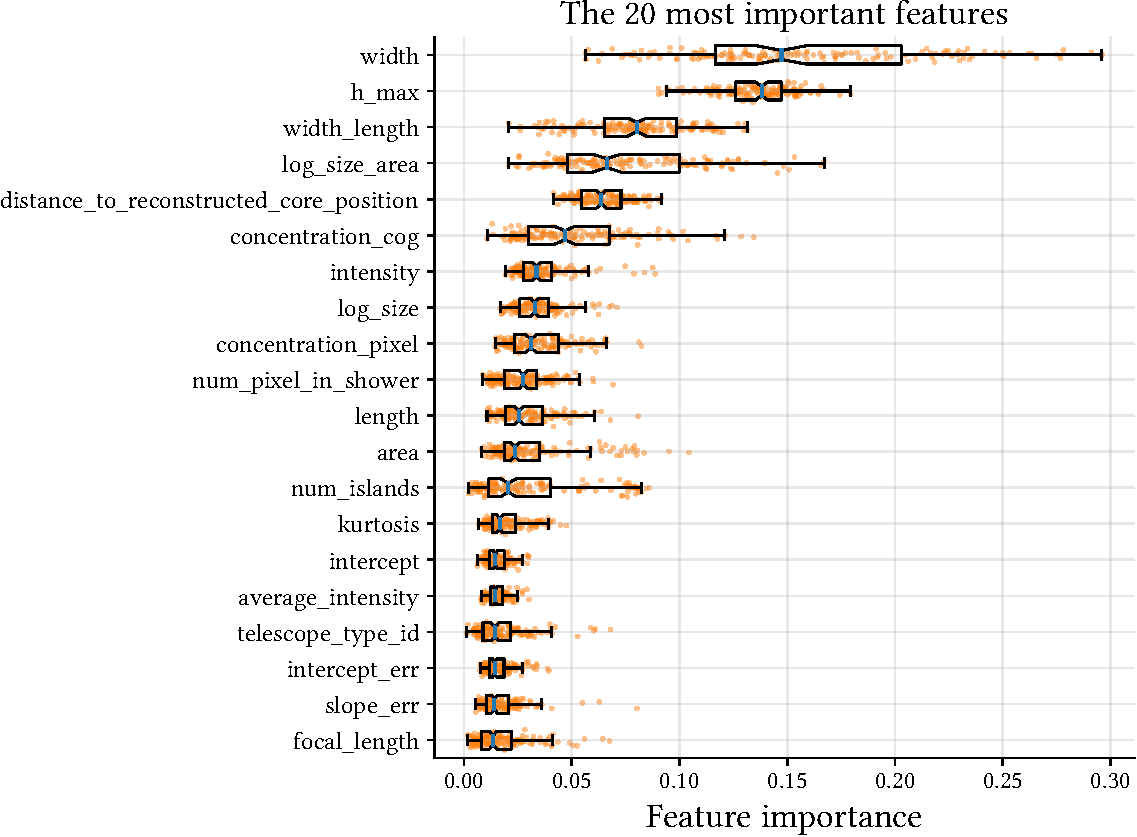
\includegraphics[page=1, width=.8\textwidth]{../analysis/plots/separation_features.pdf}
    \caption{Feature importance for the gamma/hadron separation.}
    \label{fig:gh_features}
\end{figure}


The resulting precision, recall and $f$-score are shown in figure \ref{fig:gh_fscore}.

\begin{figure}
    \centering
    \includegraphics[page=3, width=.8\textwidth]{../analysis/plots/cross_val_sep_perf_plot.pdf}
    \caption{Precision, recall and F-score for the gamma/hadron separation model on the 
    cross-validated dataset. The maximum F-score is achieved at a prediction threshold
    of $\approx \num{0.82}$.}
    \label{fig:gh_fscore}
\end{figure}

For the hadroness cut, that we apply later, we will choose the maximum of the $f_{\num{0.1}}$-score
at $\approx \num{0.82}$
\section{position}\label{position}

ADD $1/N_TEL$ LINE TO THE RES/MULTI PLOTS AND COMPARE WITH RESULTS
MENTIONED HERE:
\url{https://arxiv.org/pdf/astro-ph/9904234.pdf}

\subsection{Analysis at telescope level}

The random forests for the DISP- and SIGN-prediction get trained on
XXX diffuse gamma events with a 3-fold cross-validation.
The SIGN-model is not needed for this part, but can be useful as 
a cross-check for the LST-mono analysis in section \ref{lst mono part}.

The performance of the models can be gauged by looking at the 
figures \ref{fig:disp_test_perf} for the cross-validated set and 
\ref{fig:disp_test_perf} for the performance our 
pointlike data.

In both cases we can see that the DISP-model gets rapidly more
powerful with higher energies up until ~\SI{1}{\tera\electronvolt} from 
where on the performance stays the same.

The SIGN-model does not saturate like this and improves pretty linear up until
the highest energies.

\begin{figure}
    \begin{subfigure}{0.45\textwidth}
        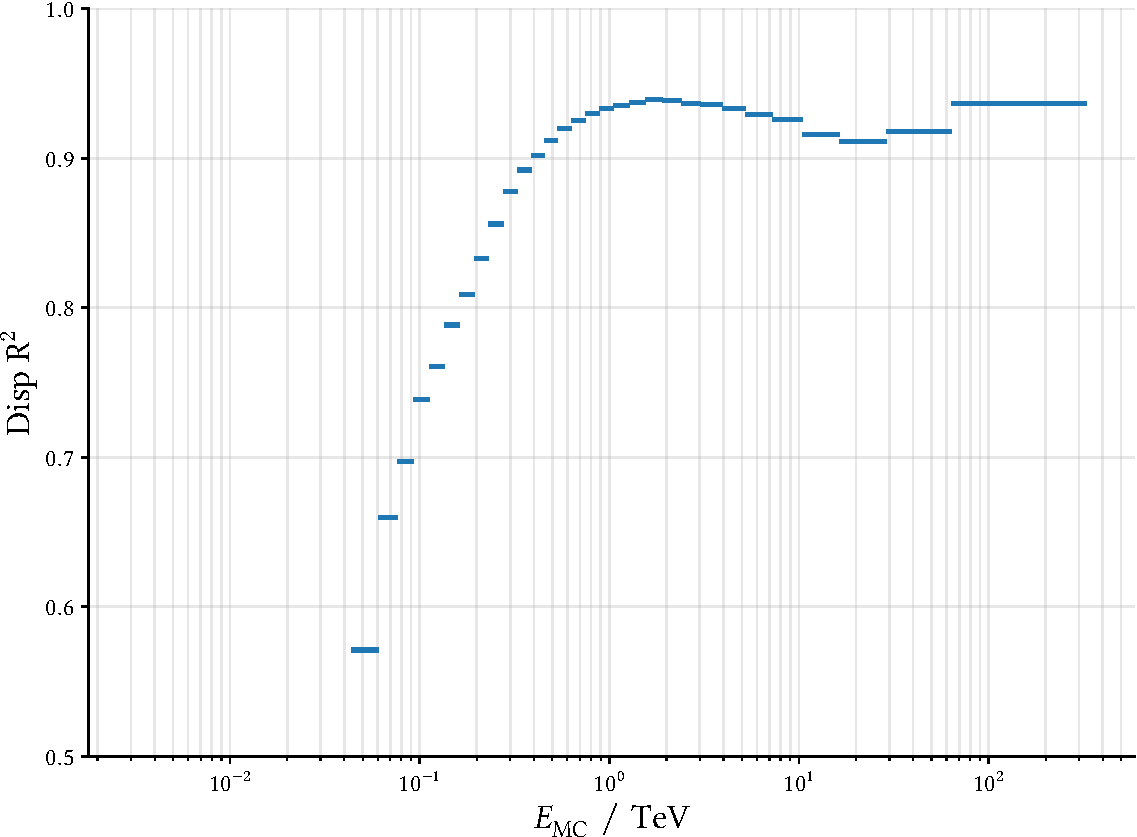
\includegraphics[width=0.9\linewidth]{../analysis/plots/disp_test_r2_equal_filled.pdf} 
        \caption{R2-Score for the DISP-estimation}
    \end{subfigure}
    \begin{subfigure}{0.45\textwidth}
        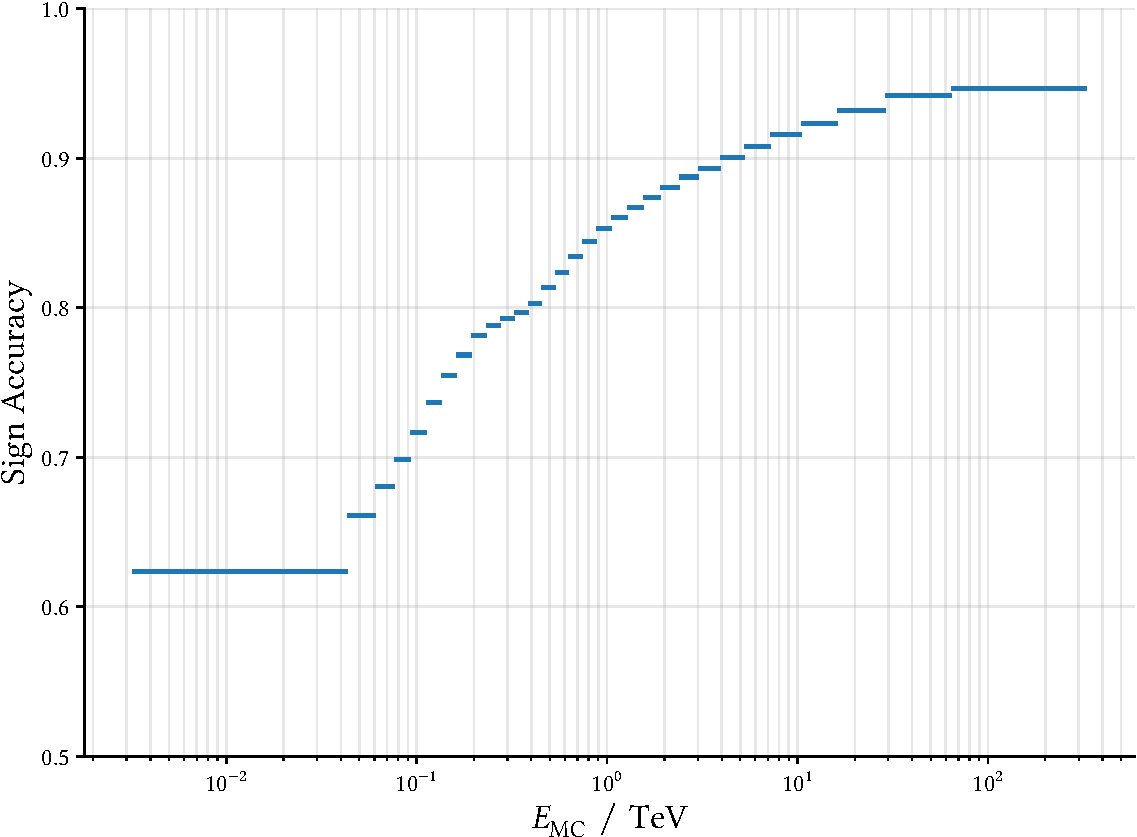
\includegraphics[width=0.9\linewidth]{../analysis/plots/disp_test_acc_equal_filled.pdf}
        \caption{SIGN-accuracy}
    \end{subfigure}
    \caption{Performance of the DISP- and SIGN-estimation algorithm on the test-dataset.}
    \label{fig:disp_test_perf}
\end{figure}

\begin{figure}
    \begin{subfigure}{0.45\textwidth}
        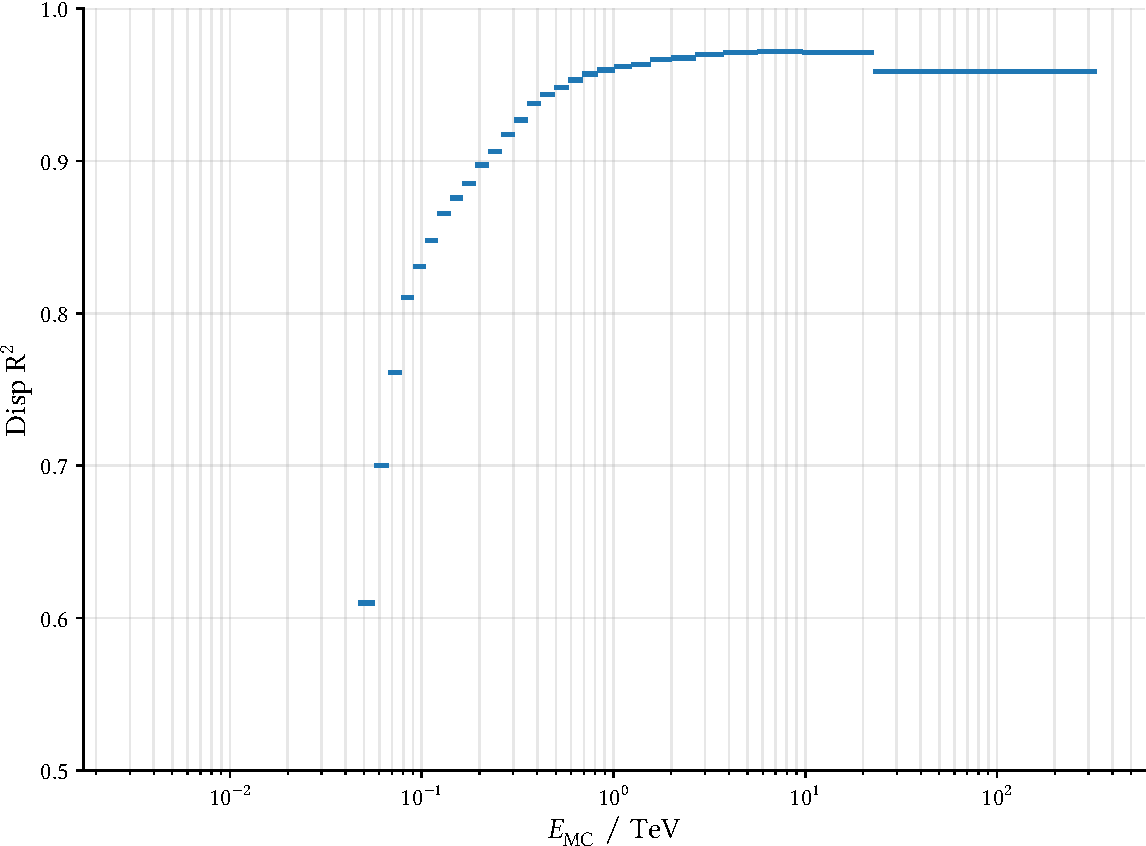
\includegraphics[width=0.9\linewidth]{../analysis/plots/disp_gamma_r2_equal_filled.pdf} 
        \caption{R2-Score for the DISP-estimation}
    \end{subfigure}
    \begin{subfigure}{0.45\textwidth}
        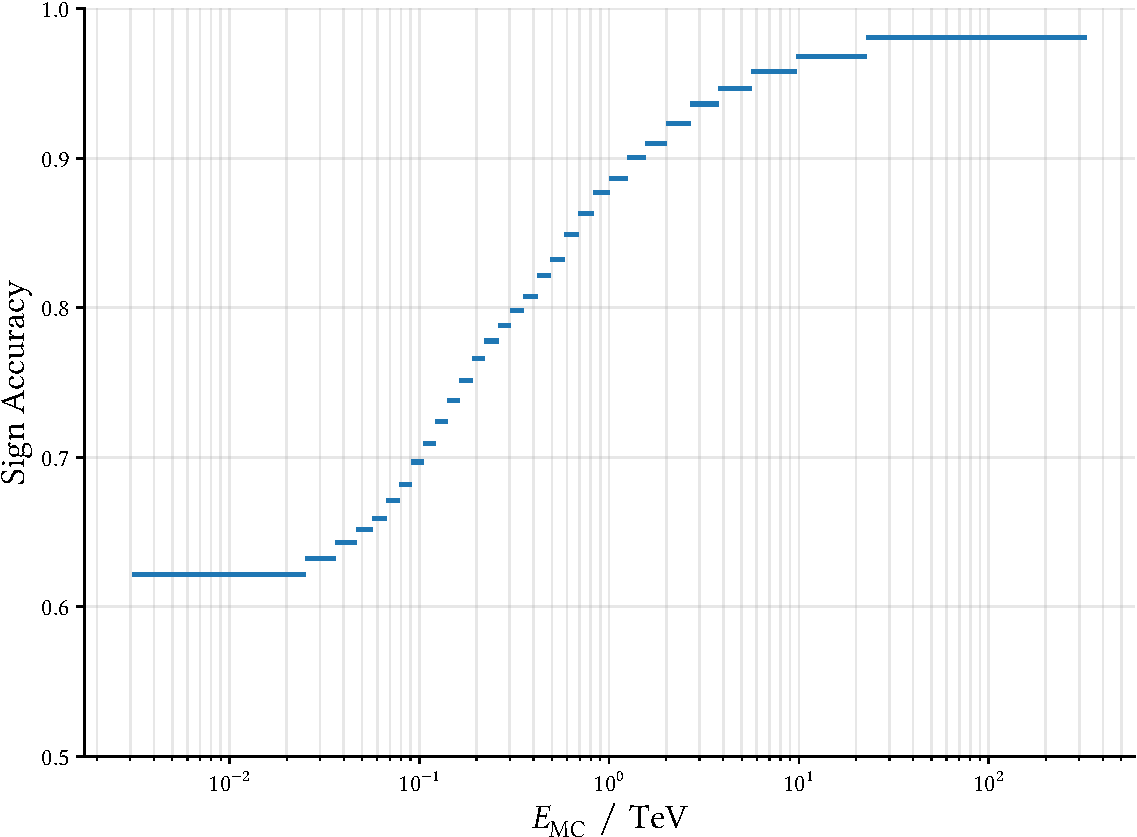
\includegraphics[width=0.9\linewidth]{../analysis/plots/disp_gamma_acc_equal_filled.pdf}
        \caption{SIGN-accuracy}
    \end{subfigure}
    \caption{Performance of the DISP- and SIGN-estimation algorithm on the pointlike dataset..}
    \label{fig:disp_gamma_perf}
\end{figure}

From figure \ref{fig:disp_features} we can learn that 
the stereoscopic features "$distance_to_reconstructed_core_position$"
and $h_max$ have a high influence on the prediction.


\begin{figure}
	\centering
	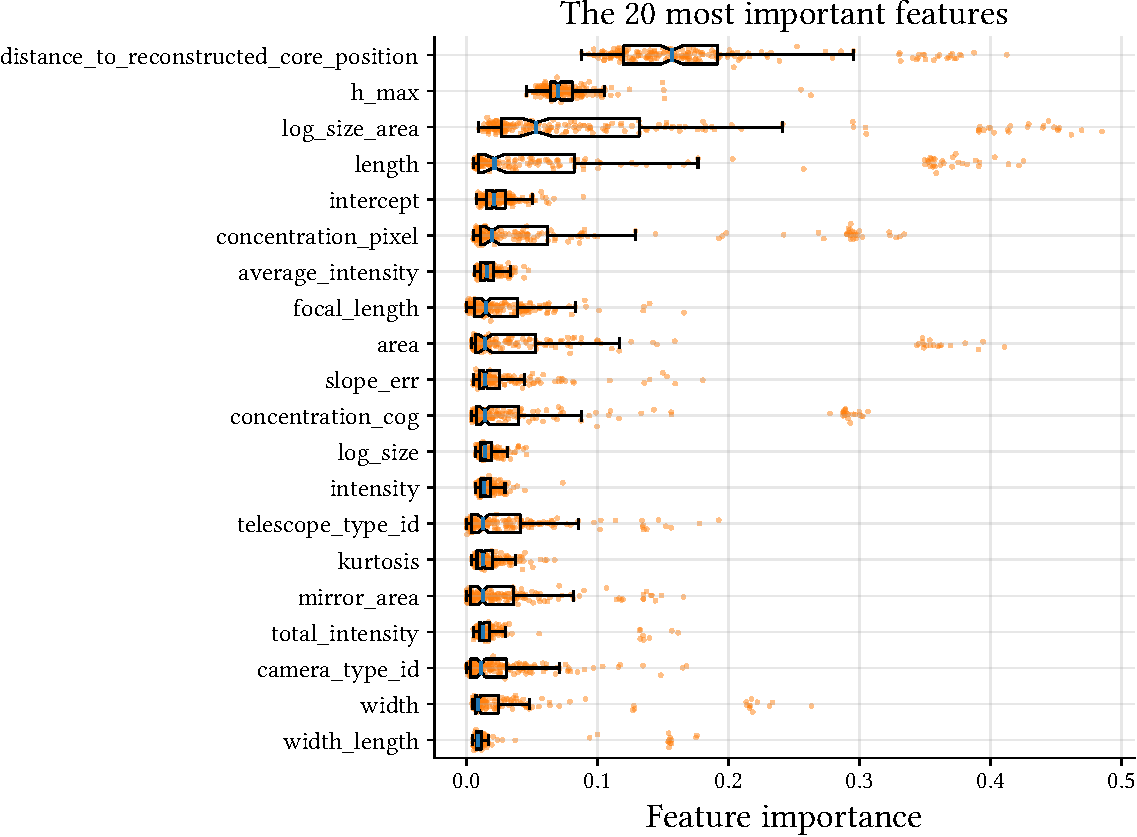
\includegraphics[width=0.8\textwidth]{../analysis/plots/disp_features.pdf}
	\caption{disp features}
	\label{fig:disp_features}
\end{figure}

The final results can be seen in figure \ref{fig:sens_telescope}.
One can derive - in accordance to the previously discussed metrics - 
that the DISP-prediction improves with increasing energies and there are less
missclassified SiGNs at higher energies.
We can also see the saturated DISP-performance at \SI{1}{\tera\electronvolt}.

\begin{figure}
    \centering
    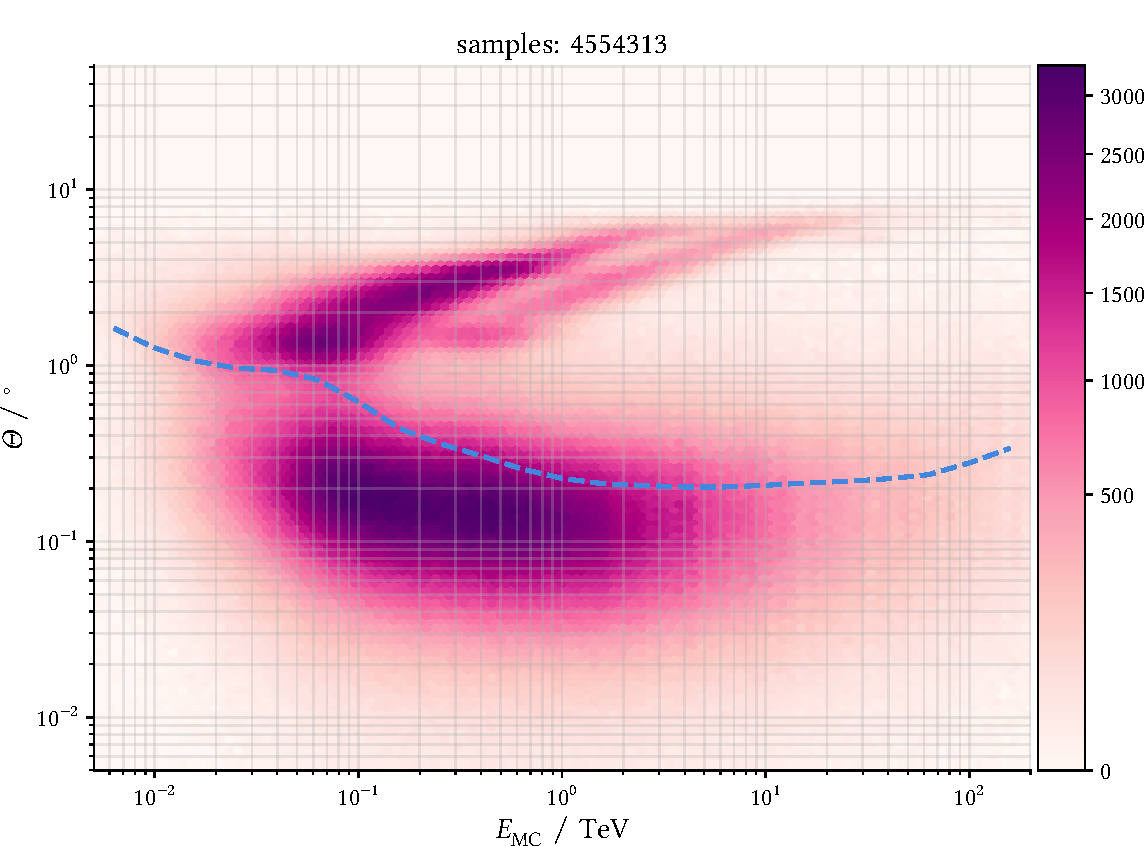
\includegraphics[width=.8\textwidth]{../analysis/plots/gamma/tel_vs_energy.pdf}
    \caption{Per telescope predictions for the source position}
    \label{fig:sens_telescope}
\end{figure}


\subsection{Analysis for the stereoscopic array}

As a baseline comparison we compare the median DISP-prediction 
with the results obtained with the Hillas-reconstructor.
These results can be seen in figure \ref{fig:stereo_double_median}.
At each energy the Hillas-reconstructor performs considerably better.
One can also see that the median predictions do not improve considerably after
\SI{3}{\tera\electronvolt} and gets worse after \SI{20}{\tera\electronvolt}.
The Hillas-reconstructor shows a similar bump at the highest energies,
so these are probably just some bad events.
It also has a short bump in the range of \SI{200}{\giga\electronvolt}
to \SI{1}{\tera\electronvolt}. This is due to a lot of multi 3 events there.
do we have a paper?

Looking at the multiplicity we can conclude that the median predictions
do not scale as well with higher multiplicities.

\begin{figure}
    \centering
    \begin{subfigure}{0.45\textwidth}
        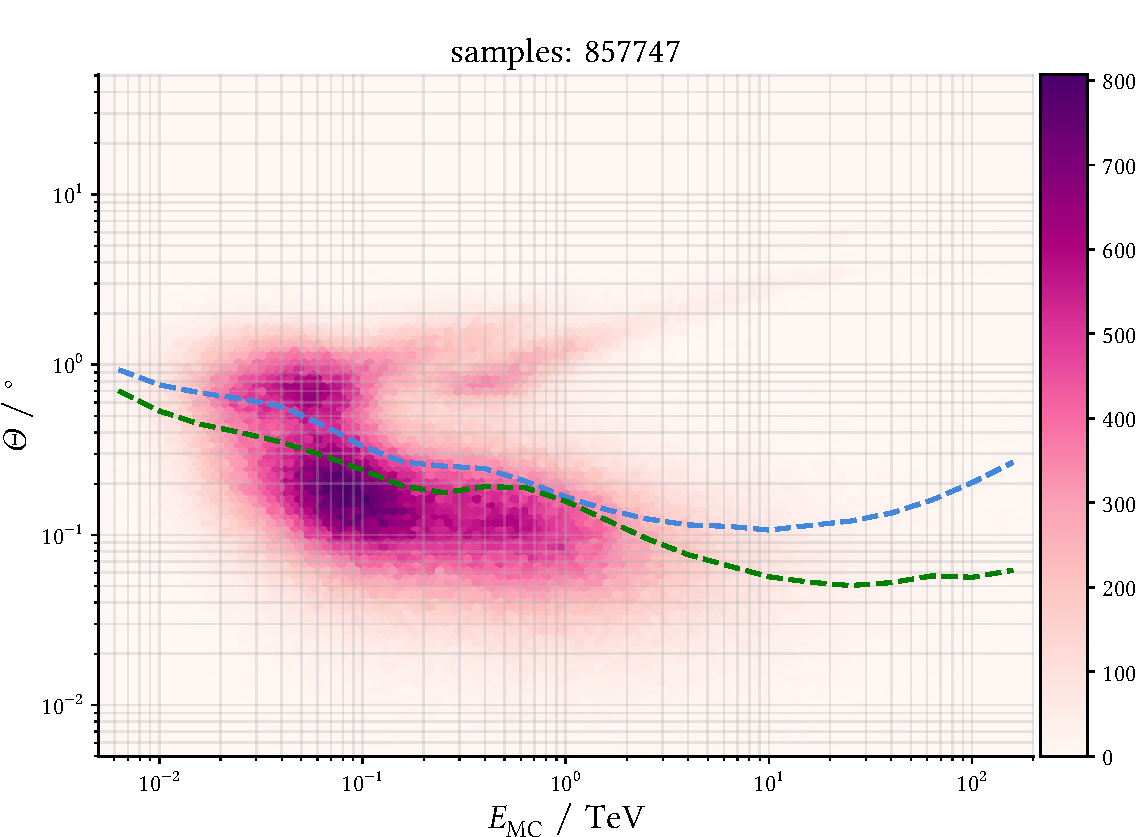
\includegraphics[width=0.9\linewidth]{../analysis/plots/gamma/median_vs_energy.pdf} 
        \caption{Distance in degree against energy}
    \end{subfigure}
    \begin{subfigure}{0.45\textwidth}
        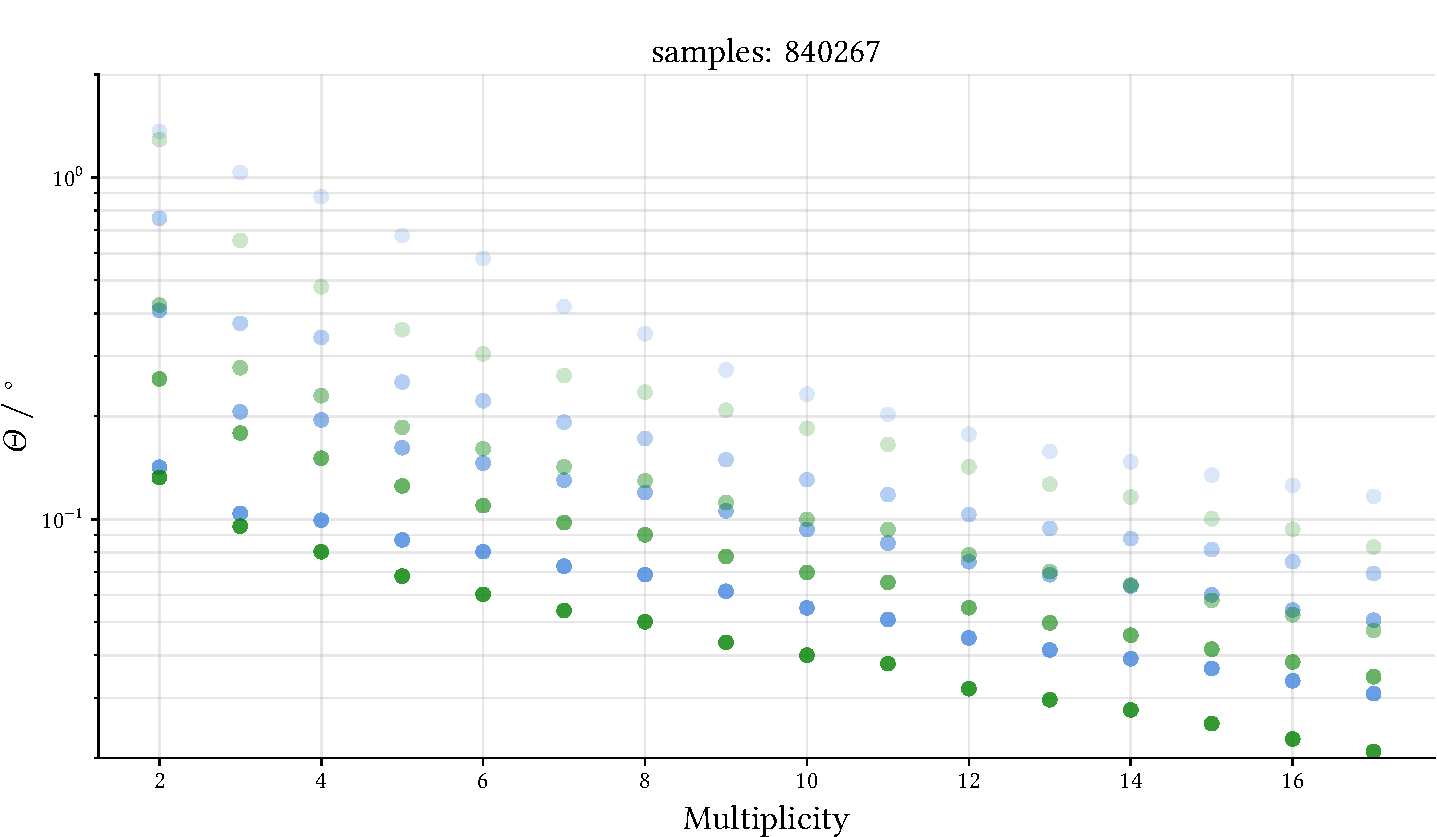
\includegraphics[width=0.9\linewidth]{../analysis/plots/gamma/median_vs_multi_comp.pdf}
        \caption{Distance in degree against multiplicity}
    \end{subfigure}
    \caption{Performance of the median telescope prediction compared 
    against the Hillas-Reconstructor. Median in Blue, Hillas in green. bins from median, hillas
    line extra}
    \label{fig:stereo_double_median}
\end{figure}

The results of the more sophisticated DISP-approach can be seen in figure \ref{fig:stereo_double_magic}.
Compared to figure \ref{fig:stereo_double_median} the completely misreconstructed events are almost
gone and the 68\% percentile is much improved throughout the complete energy range despite 
the very highest energies. At this point the DISP-error is probably limiting and the 
Hillas-reconstructor leads to much better results.
At the lower energy range our approach seems to be working pretty well, 
slightly outperforming the Hillas-reconstructor.
When looking at the multiplicity-plot, we see a similar picture as before but with 
better results. At high multiplicities $\ge 3$ the Hillas-reconstructor 
leads to better results. Improvements can be seen especially at 2-multiplicity 
events. In that case the iterative approach is identical to the 
base Magic-method.
The Hillas-reconstructor on the other hand does not work too well with 2 
triggered telescopes, with 3 triggered telescopes leading to much better results 
already.


\begin{figure}
    \centering
    \begin{subfigure}{0.45\textwidth}
        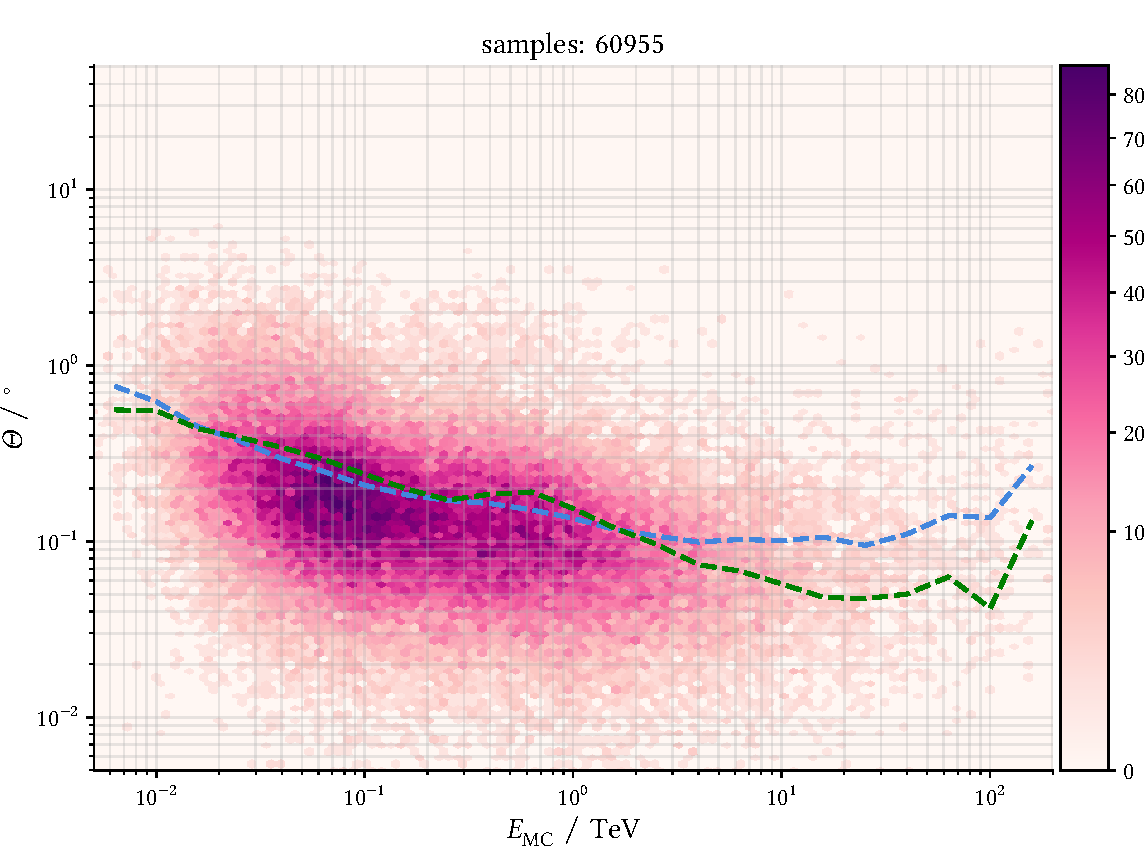
\includegraphics[width=0.9\linewidth]{../analysis/plots/gamma/pairwise_median_100_vs_energy.pdf} 
        \caption{Distance in degree against energy}
    \end{subfigure}
    \begin{subfigure}{0.45\textwidth}
        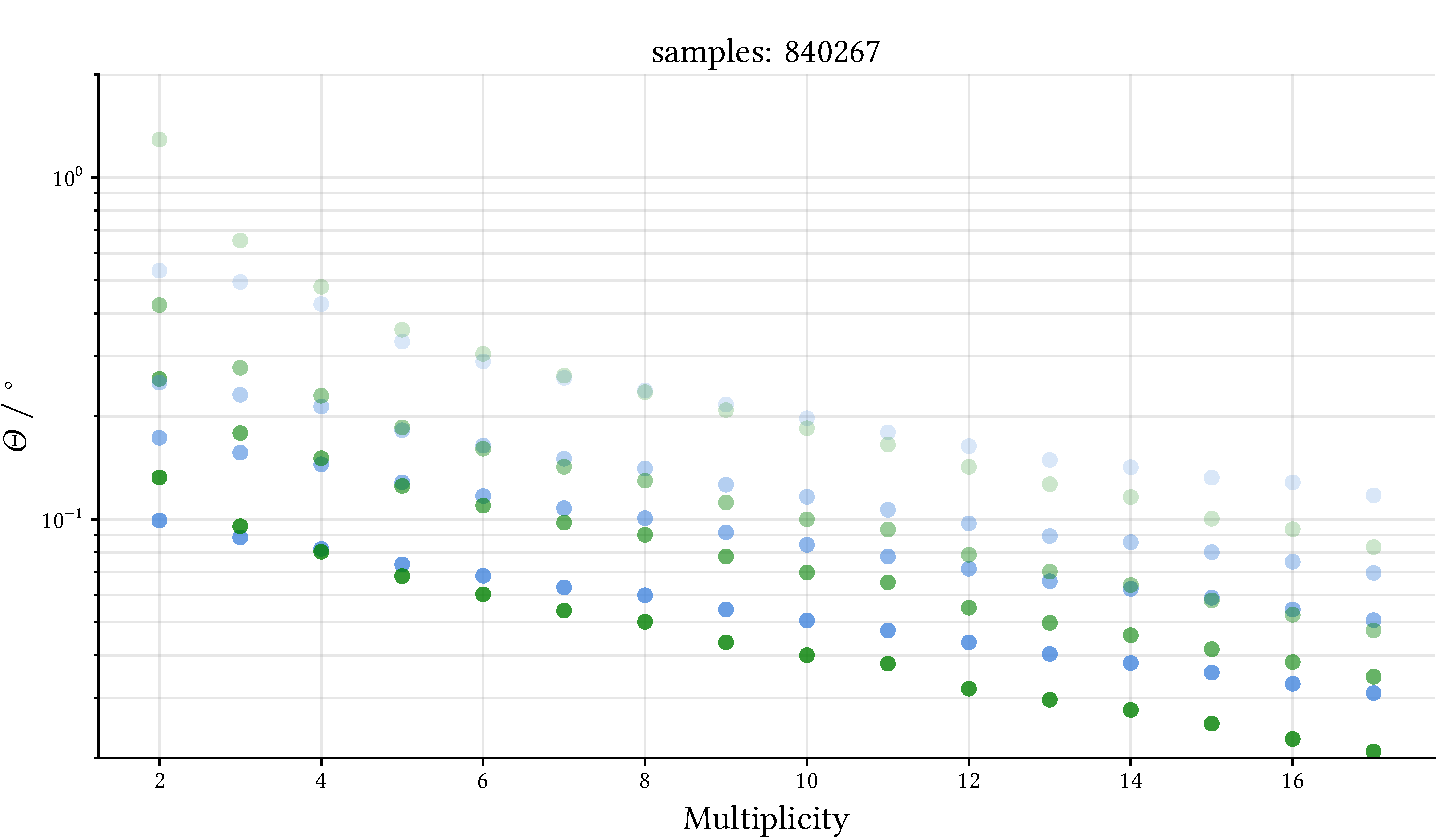
\includegraphics[width=0.9\linewidth]{../analysis/plots/gamma/pairwise_median_100_vs_multi_comp.pdf}
        \caption{Distance in degree against multiplicity}
    \end{subfigure}
    \caption{Performance of the superduper compared 
    against the Hillas-Reconstructor. Median in Blue, Hillas in green
    Actually better, but in the extreme regions where statistics is low as well.}
    \label{fig:stereo_double_magic}
\end{figure}


\section{hadroness cut}

In a analysis of real data, some legitimate events usually get discarded
in the gamma-/hadron-separation step.
Assuming that the misclassified events are in some way non regular, it might be 
justified to assume that these events also behave abnormal during the reconstruction of 
the source position. Discarding these events could thus improve the overall 
predictions.

The predictions of the gamma-/hadron-separation model on the cross-validated dataset
are summarized in figure \ref{plot aus aict tools!}.
Based on this performance we set the gammaness cut at XXX.


With this cut XXX events remain.
\begin{figure}
    \centering
    \begin{subfigure}{0.45\textwidth}
        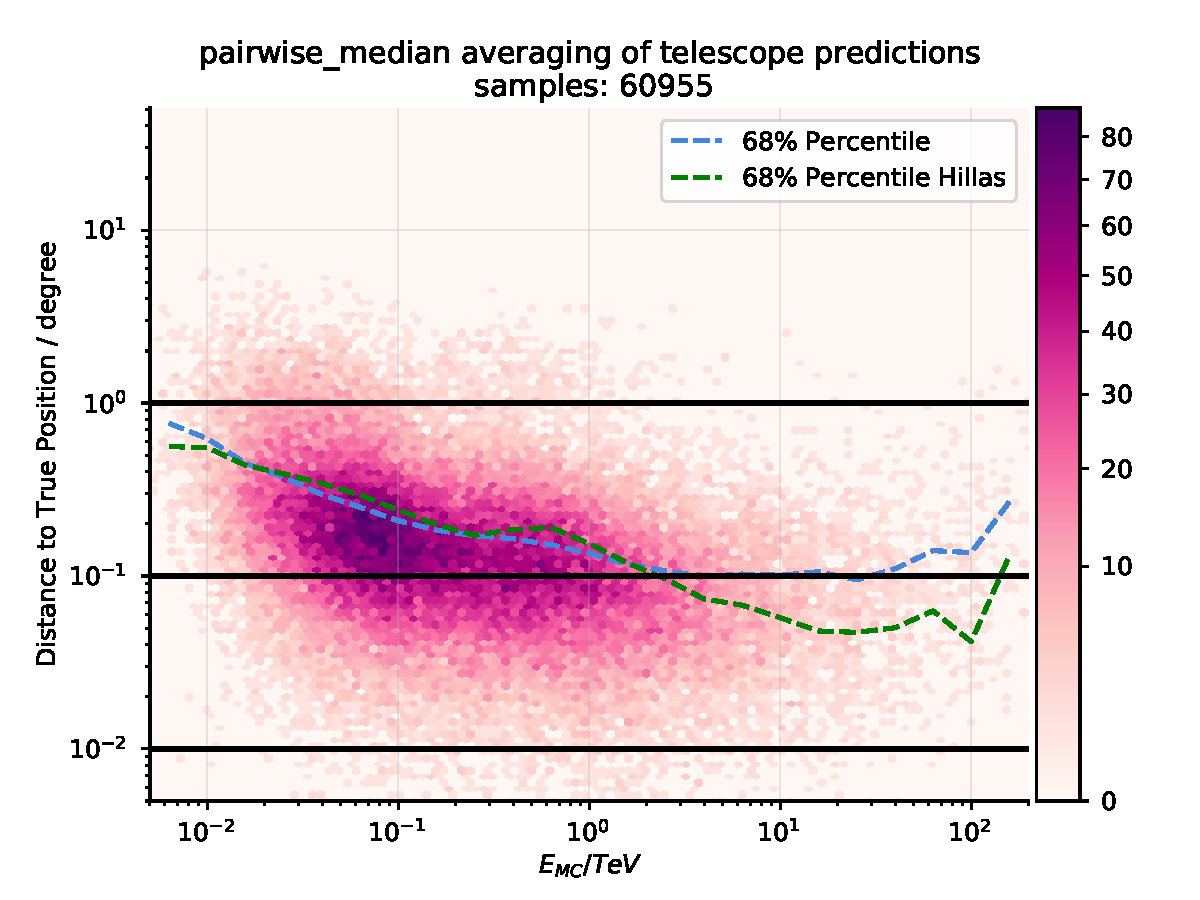
\includegraphics[width=0.9\linewidth]{../analysis/plots/gamma_cut/pairwise_median_100_vs_energy.pdf} 
        \caption{Distance in degree against energy}
    \end{subfigure}
    \begin{subfigure}{0.45\textwidth}
        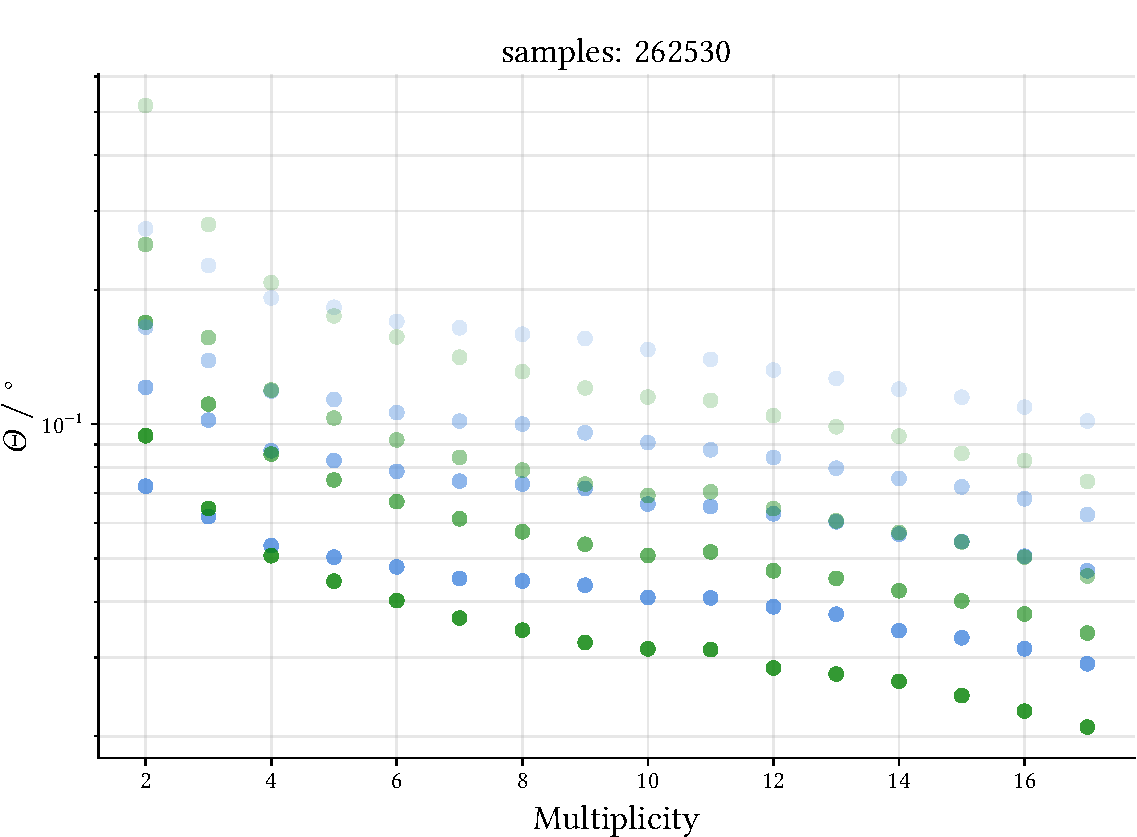
\includegraphics[width=0.9\linewidth]{../analysis/plots/gamma_cut/pairwise_median_100_vs_multi_comp.pdf}
        \caption{Distance in degree against multiplicity}
    \end{subfigure}
    \caption{Performance of the superduper compared 
    against the Hillas-Reconstructor. Median in Blue, Hillas in green
    Actually better, but in the extreme regions where statistics is low as well.}
    \label{fig:stereo_double}
\end{figure}


-> bringt nichts?


\section{LST only}
To simulate early operation stages where the LST1 is the only fully functional 
telescope, the analysis is limited to only the single LST with 
the simtel id 4.

This means that we do not have a baseline Hillas Reconstructor as we can not use
stereoscopy and each array event holds exactly one telescope event.
We expect to
get a similar sensitivity as in the earlier figure \ref{fig:sens_telescope}.

We also limit the training data, so we will have trained on less samples as well.

HOW DOES THE PERFORMANCE CHANGE?
THIS REQUIRES MORE EVENTS AND MAYBE MORE LSTS FOR TRAINING?

\begin{figure}
    \begin{subfigure}{0.45\textwidth}
        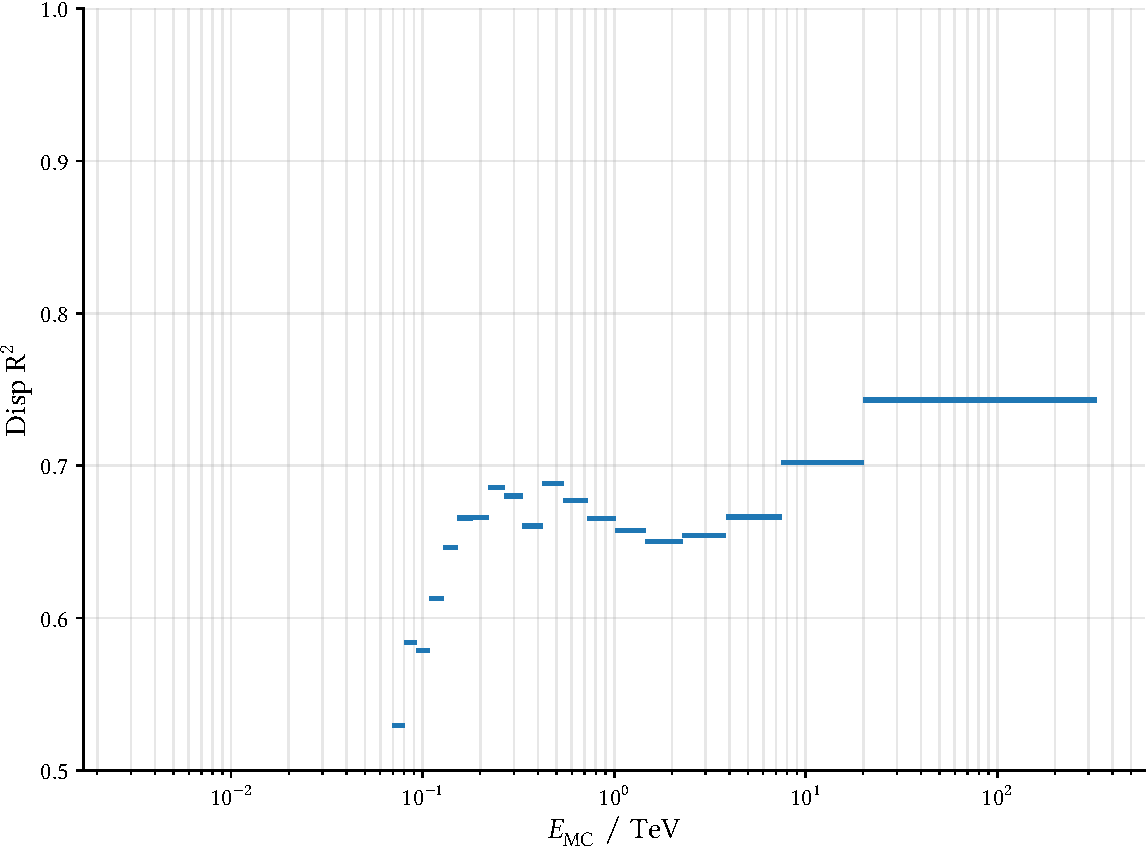
\includegraphics[width=0.9\linewidth]{../analysis/plots/disp_test_mono_lst_r2_equal_filled.pdf} 
        \caption{R2-Score for the DISP-estimation}
    \end{subfigure}
    \begin{subfigure}{0.45\textwidth}
        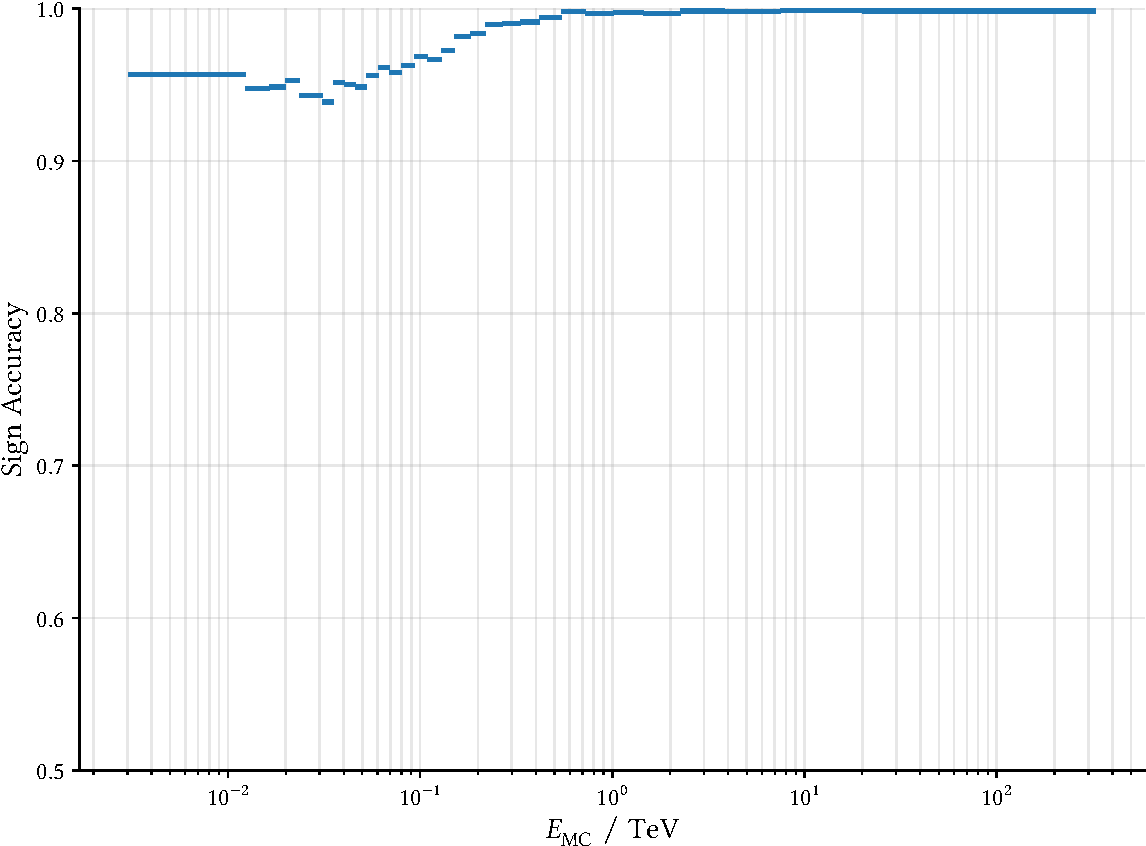
\includegraphics[width=0.9\linewidth]{../analysis/plots/disp_test_mono_lst_acc_equal_filled.pdf}
        \caption{SIGN-accuracy}
    \end{subfigure}
    \caption{Performance of the DISP- and SIGN-estimation algorithm on the test-dataset.}
    \label{fig:disp_test_perf}
\end{figure}

\begin{figure}
    \begin{subfigure}{0.45\textwidth}
        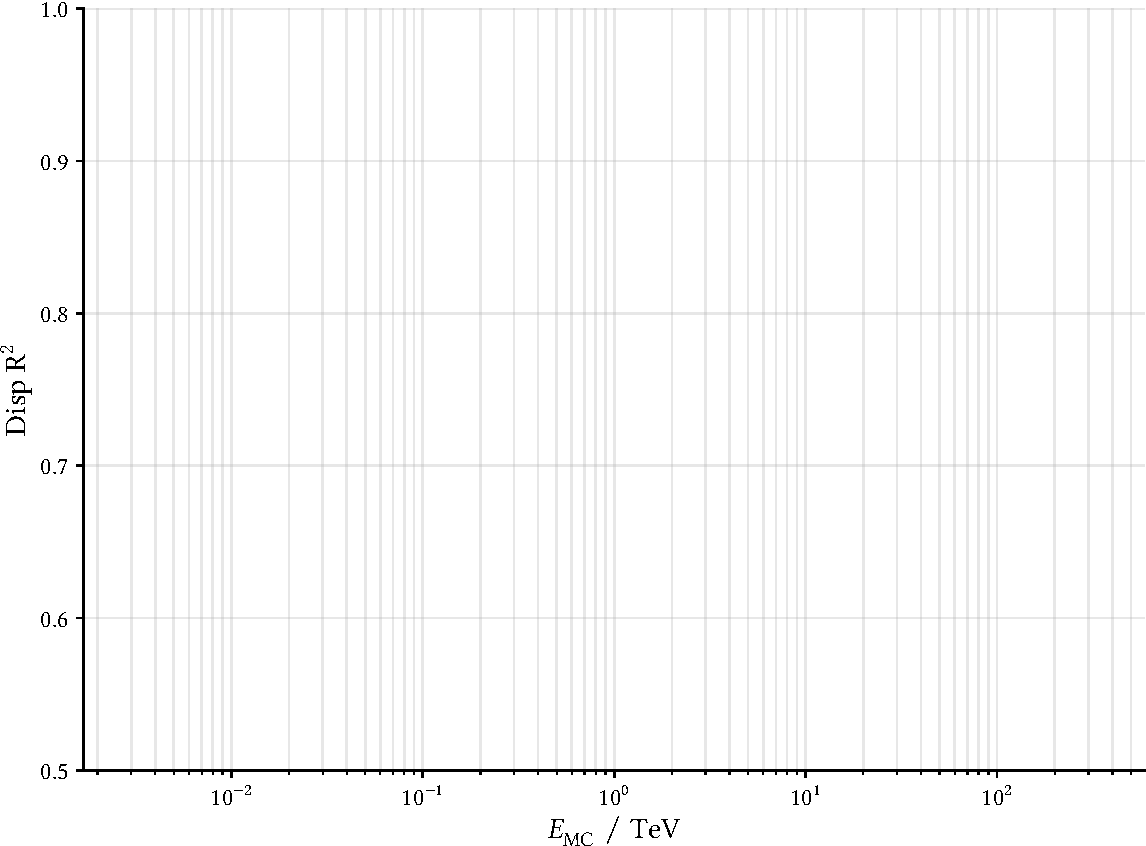
\includegraphics[width=0.9\linewidth]{../analysis/plots/disp_gamma_mono_lst_r2_equal_filled.pdf} 
        \caption{R2-Score for the DISP-estimation}
    \end{subfigure}
    \begin{subfigure}{0.45\textwidth}
        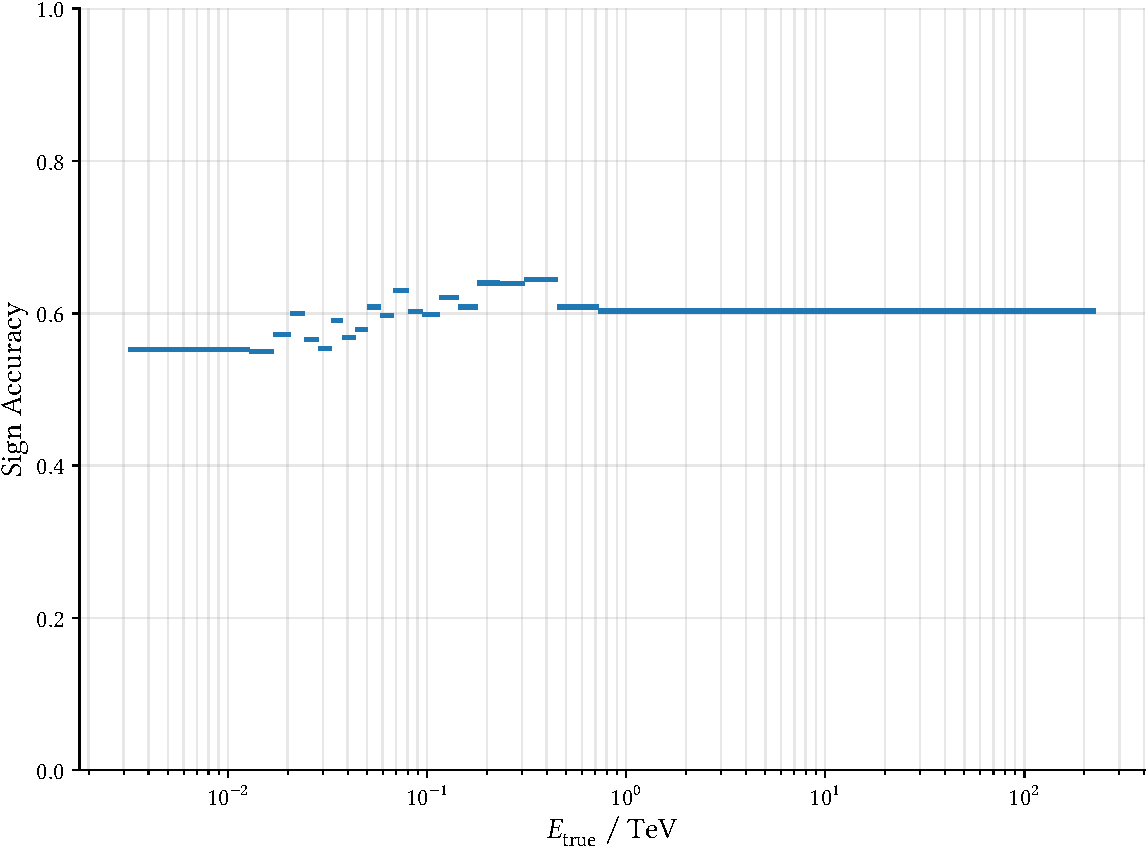
\includegraphics[width=0.9\linewidth]{../analysis/plots/disp_gamma_mono_lst_acc_equal_filled.pdf}
        \caption{SIGN-accuracy}
    \end{subfigure}
    \caption{Performance of the DISP- and SIGN-estimation algorithm on the pointlike dataset..}
    \label{fig:disp_gamma_perf}
\end{figure}

Looks decent, energy obviously limited bc LST.

\chapter{energy}\label{energy}

ToDo:
\begin{enumerate}[nosep]
    \item Erklärung Features
    \item Trainingsperformance + daten
    \item Ergebnisse Mono
    \item Ergebnisse Stereo
\end{enumerate}


\chapter{conclusion}\label{conclusion}
ToDo:
\begin{enumerate}[nosep]
    \item ???
    \item ausbblick: andere lerner? adaboost?
\end{enumerate}


%\appendix
% Hier beginnt der Anhang, nummeriert in lateinischen Buchstaben
%\chapter{Ein Anhangskapitel}

Hier könnte ein Anhang stehen, falls Sie z.\,B.\ Code, Konstruktionszeichnungen oder Ähnliches mit in die Arbeit bringen wollen.
Im Normalfall stehen jedoch alle Ihre Resultate im Hauptteil der Bachelorarbeit und ein Anhang ist überflüssig.


\backmatter
\printbibliography

\cleardoublepage
\thispagestyle{empty}
\section*{Eidesstattliche Versicherung}
Ich versichere hiermit an Eides statt, dass ich die vorliegende Abschlussarbeit mit dem Titel \enquote{\thetitle} selbstständig und ohne unzulässige fremde Hilfe erbracht habe.
Ich habe keine anderen als die angegebenen Quellen und Hilfsmittel benutzt, sowie wörtliche und sinngemäße Zitate kenntlich gemacht. 
Die Arbeit hat in gleicher oder ähnlicher Form noch keiner Prüfungsbehörde vorgelegen.

\vspace*{1cm}\noindent
\begin{center}
  \begin{tabular}{@{}p{0.4\textwidth}@{\hspace{0.15\textwidth}}p{0.4\textwidth}@{}}
  \rule{\linewidth}{0.25pt}& \rule{\linewidth}{0.25pt}\\
  Ort, Datum & Unterschrift
  \end{tabular}
\end{center}

\subsection*{Belehrung}
Wer vorsätzlich gegen eine die Täuschung über Prüfungsleistungen betreffende Regelung einer Hochschulprüfungsordnung verstößt, handelt ordnungswidrig.
Die Ordnungswidrigkeit kann mit einer Geldbuße von bis zu \SI[round-mode=places, round-precision=2]{50000}{€} geahndet werden. 
Zuständige Verwaltungsbehörde für die Verfolgung und Ahndung von Ordnungswidrigkeiten ist der Kanzler/die Kanzlerin der Technischen Universität Dortmund. 
Im Falle eines mehrfachen oder sonstigen schwerwiegenden Täuschungsversuches kann der Prüfling zudem exmatrikuliert werden \mbox{(\S\,63 Abs. 5 Hochschulgesetz --HG--).}

Die Abgabe einer falschen Versicherung an Eides statt wird mit Freiheitsstrafe bis zu 3 Jahren oder mit Geldstrafe bestraft.

Die Technische Universität Dortmund wird ggf.\ elektronische Vergleichswerkzeuge (wie z.\,B.\ die Software \enquote{turnitin}) zur Überprüfung von Ordnungswidrigkeiten in Prüfungsverfahren nutzen. \\[\baselineskip]

\noindent Die oben stehende Belehrung habe ich zur Kenntnis genommen.\\[1cm]
\begin{center}
\begin{tabular}{@{}p{0.4\textwidth}@{\hspace{0.15\textwidth}}p{0.4\textwidth}@{}}
\rule{\linewidth}{0.25pt}& \rule{\linewidth}{0.25pt}\\
Ort, Datum & Unterschrift
\end{tabular}
\end{center}

\end{document}
